\chapter{Timing study of hadronic showers in the AHCAL technological prototype}
\label{chap:TimingAHCAL}

The International Large Detector (ILD), as described in \ref{}, considers a highly granular hadronic calorimeter using iron absorbers to achieve a compact detector with the best jet energy resolution around 3-4\% at 250 GeV satisfying the space constrain imposed by the solenoid magnet. Timing measurements in a calorimeter can be used to reject pile-up events, for example at the LHC or CLIC coming from out-of-time pile-up events due to the bunch-to-bunch spacing of 25 (0.5 ns) respectively. The high level of $\gamma\gamma \rightarrow$ hadrons events could be rejected by using the timing information from the calorimeter in order to limit the impact of the background on physics measurements. Many novel techniques to use time information for improving energy reconstruction could be used \cite{Benaglia2016}.\\

In the hadronic calorimeter, the timing precision is highly influenced by the time structure of the shower itself. A hadronic shower possesses several timing components depending on the different processes happening in the shower. A fast component related to instantaneous high energy depositions from relativistic hadrons and electromagnetic sub-showers. A slow component due to neutron scattering, nuclear-recoil and photons from nuclear processes. This component can live up to several milliseconds. Apart from physics processes, the measured hit time is influenced by the active medium used as well as by the electronics. Time constants in the active medium, such as scintillation decay time, can affect the measurement.\\

The performance of the ILD relies on simulation studies based on \geant, it is important to study how well the simulation performs to reproduce the time structure of hadronic showers observed in data. The CALICE Analog Hadronic Calorimeter (AHCAL) technological prototype was installed at the SPS CERN facilities in July and August 2015, in order to provide measurements using plastic scintillators. The goal of this study is to improve our knowledge about hadronic showers, especially in terms of its time evolution and the time correlations between layers within the calorimeter. This chapter will firstly describe the timing calibration procedure of the AHCAL, followed by the comparison between data and simulation for muons and electrons and finally a comparison with pion data.

\section{Runs \& Event Selection}
\label{sec:EvtSelection}

\subsection{Trigger Signals}
\label{subsec:trigger}

For a muon beam, two scintillator plates of $50\times50$ cm$^2$ were placed in front and back of the calorimeter. For electron and pion beams, two small scintillator plates of $10\times10$ cm$^2$ were positioned in front of the calorimeter. The trigger scintillators were connected to a NIM-logic (discriminator and gate) in order to provide a validation signal to the chip.
In order to provide the time reference of the trigger scintillators, a SiPM-like pulse of around 4 $\mu$s length and with a fast rising edge of around 1 ns was generated from the NIM-logic. This signal was injected directly via AC coupling to some channels in the setup as shown in the table \ref{table:trigger_signal_list}. No other external time reference than these channels was available. In the following analysis, only the reference signals T$_{12}$,  T$_{13}$ and T$_{14}$ were used.

\begin{table}[htb!]
	\centering
	\caption{List of channels with the injected trigger signal to be used as time reference.}
	\label{table:trigger_signal_list}
	\begin{tabular}{@{} ccccc @{}}
		\hline
		Layer \# & Chip Number & Channel & Comments & Appellation \\
		\hline
		11 & 169 & 29 & noisy & T$_{11}$ \\
		11 & 177 & 23 & broken & - \\
		12 & 185 & 29 & - & T$_{12}$ \\
		13 & 201 & 29 & -  & T$_{13}$ \\
		13 & 211 & 6 & broken & - \\
		14 & 217 & 23 & - & T$_{14}$ \\
		\hline
	\end{tabular}
\end{table}

\subsection{Dataset}
\label{subsec:dataset}

During the campaign at SPS in July 2015, $\mu^-$ runs were taken at 50 and 150 GeV beam energy for the calibration of the detector. Several e$^{-}$ runs were taken between 10 to 50 GeV beam energy to study the electromagnetic response of the calorimeter. The e$^{-}$ runs were quite pure as the beam was generated via a neutral beam directed on a converter target. Due to the significant amount of air and beam line instrumentation between the calorimeter and the final momentum selection magnet as well as few information of the beam parameters, the beam profile of electron runs is not well reproduced in simulation. Finally, $\pi^-$ runs were taken between 10 to 90 GeV beam energy. The table \ref{table:dataruns} sums up the dataset taken.

\begin{table}[htb!]
	\centering
	\caption{List of runs taken at SPS in July 2015.}
	\label{table:dataruns}
	\resizebox{0.8\textwidth}{!}{%
	\begin{tabular}{@{}l||p{2cm}p{8cm}@{}}
		\hline
		\multicolumn{1}{l}{\textbf{Particle}} & \textbf{Energy} & \textbf{Runs}\\
		\hline
		\multirow{2}{*}{$\mu^-$}& 50 GeV & 24016-24204\\& 150 GeV & 24623-24662\\
		\hline
		\multirow{2}{*}{e$^-$}& 10 GeV & 24531-24576\\& 15 GeV & 24507-24527\\& 20 GeV & 24479-24504\\& 30 GeV & 24454-24475\\& 40 GeV & 24420-24448\\& 50 GeV & 24404-24419\\
		\hline
		\multirow{2}{*}{$\pi^-$}& 10 GeV & 24266-24272, 24300-24317, 24381-24397\\& 20 GeV & 24398-24400\\& 30 GeV & 24259-24299, 24319-24380\\& 50 GeV & 24212-24254, 24325-24357, 24580-24612\\& 70 GeV & 24219-24242, 24365-24374\\& 90 GeV & 24233-24287, 24331-24364\\
		\hline
	\end{tabular}
	}
\end{table}

\subsection{MIP Pre-selection}
\label{subsec:Muon_presel}

A clean selection of MIP tracks is needed in order to obtain and cross-check the MIP calibration at a single cell level. A simple pre-selection was performed on the muon sample designed to select effectively MIP-like particles going through the AHCAL. In a second step, a track selection was performed to retain only MIP-like particle as explained in subsection \ref{subsec:Muon_sel}.

The pre-selection is based on the center of gravity $cog_Z$ and the number of hits $n_{Hits}$. A MIP-like particle should, in principle, deposit the same energy in each layer of the calorimeter thus the center of gravity should be roughly centered in the calorimeter in the z coordinate. As well, the number of hits should be around 1 per layer for a MIP-like particle plus accounting for some possible noise in the detector thus explaining the cut at $n_{Hits} = 20$.

The AHCAL distribution of $cog_Z$ vs $n_{Hits}$ obtained from simulated 50 GeV muons, electrons and pions and the applied pre-selection is shown in figure \ref{fig:Muons_CoGZ_nHits}. The pre-selection efficiency is 99.4\% for muons, 0\% for electrons and 13.3\% for pions. Unfortunately, some contamination of late pion showers is still present but is further reduced in the MIP selection using a track-finder.

\begin{figure}[htbp!]
	\centering
	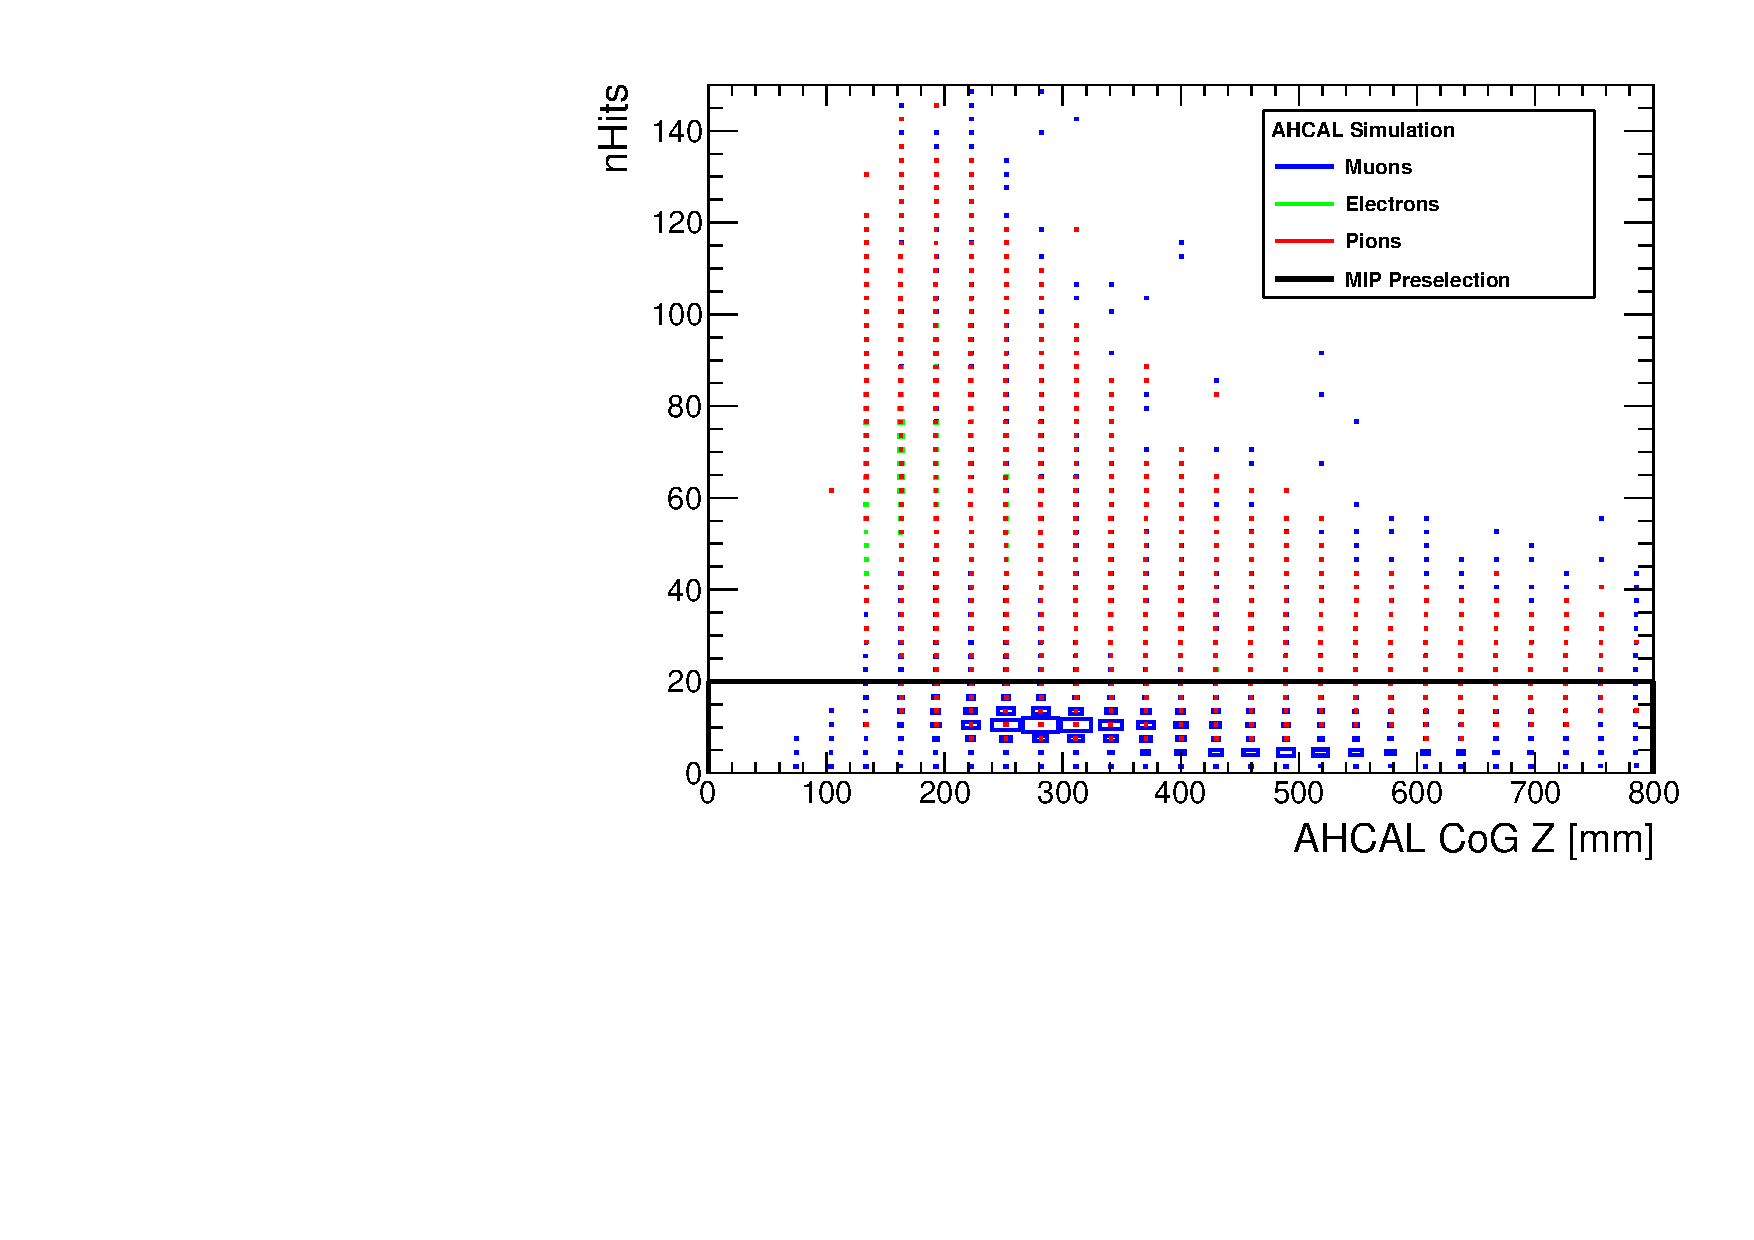
\includegraphics[width=0.5\linewidth]{chap5/fig_AHCAL_timing/Muons/SelectionCut_nHitsCoGZ_Muons}
	\caption{Event distribution in $cog_Z:n_{Hits}$ plane. The black box represents the space-phase covered by the pre-selection.} \label{fig:Muons_CoGZ_nHits}
\end{figure}

\subsection{MIP Selection}
\label{subsec:Muon_sel}

The muon runs were taken first at 50 GeV then another scan at the end of the campaign was performed at 150 GeV. The muon beam was produced by scrapping the halo of a secondary pion beam using collimators. After investigation, muon runs were contaminated by pions showers especially late and passing though the pre-selection due to the small number of active layers in the back of the calorimeter. A simple estimation provided that around 30\% of the events were contaminated.

The muon selection was designed to efficiently select muons and reject late pion showers. For this, a simple MIP track-finder has been developed based on pre-existing work \cite{Hartbrich:2016bbz}. The algorithm selects AHCAL towers of hits in the same $x:y$ plane and rejects towers under a certain number of hits. In order to select muons or punch-through pions, a straight track of at least 7 hits is required in the whole AHCAL without a hard interaction. This also assumes that the calorimeter was perfectly perpendicular to the beam, any angled tracks would be missed. In addition to reject late pion showers, not more than 2 hits are required per layer accounting for some flexibility with noise hits. The distributions of the maximum number of hits in a layer and the number of hits of a track are shown in figures \ref{fig:Muons_Track_nHitsLayer} and \ref{fig:Muons_Track_nHits} for simulated samples of 50 GeV muons, electrons and pions after pre-selection. The track-finder was performed in two steps for the inner part of the detector of $12 \times 12$ tiles and the outer part of the big layers (BL) in order to catch the halo of muons.

The selection efficiency is 72.5\% for muons, 0\% for electrons and 5.6\% for pions. The selection effectively reduces the contamination of late pion showers by over 50\% and the remaining pion efficiency is well compatible with the fraction of pions traversing the AHCAL without hard interaction. A detailed overview of the MIP selection is given in table \ref{table:muon_sel}.

\begin{figure}[htbp!]
	\begin{subfigure}[t]{0.5\textwidth}
		\centering
		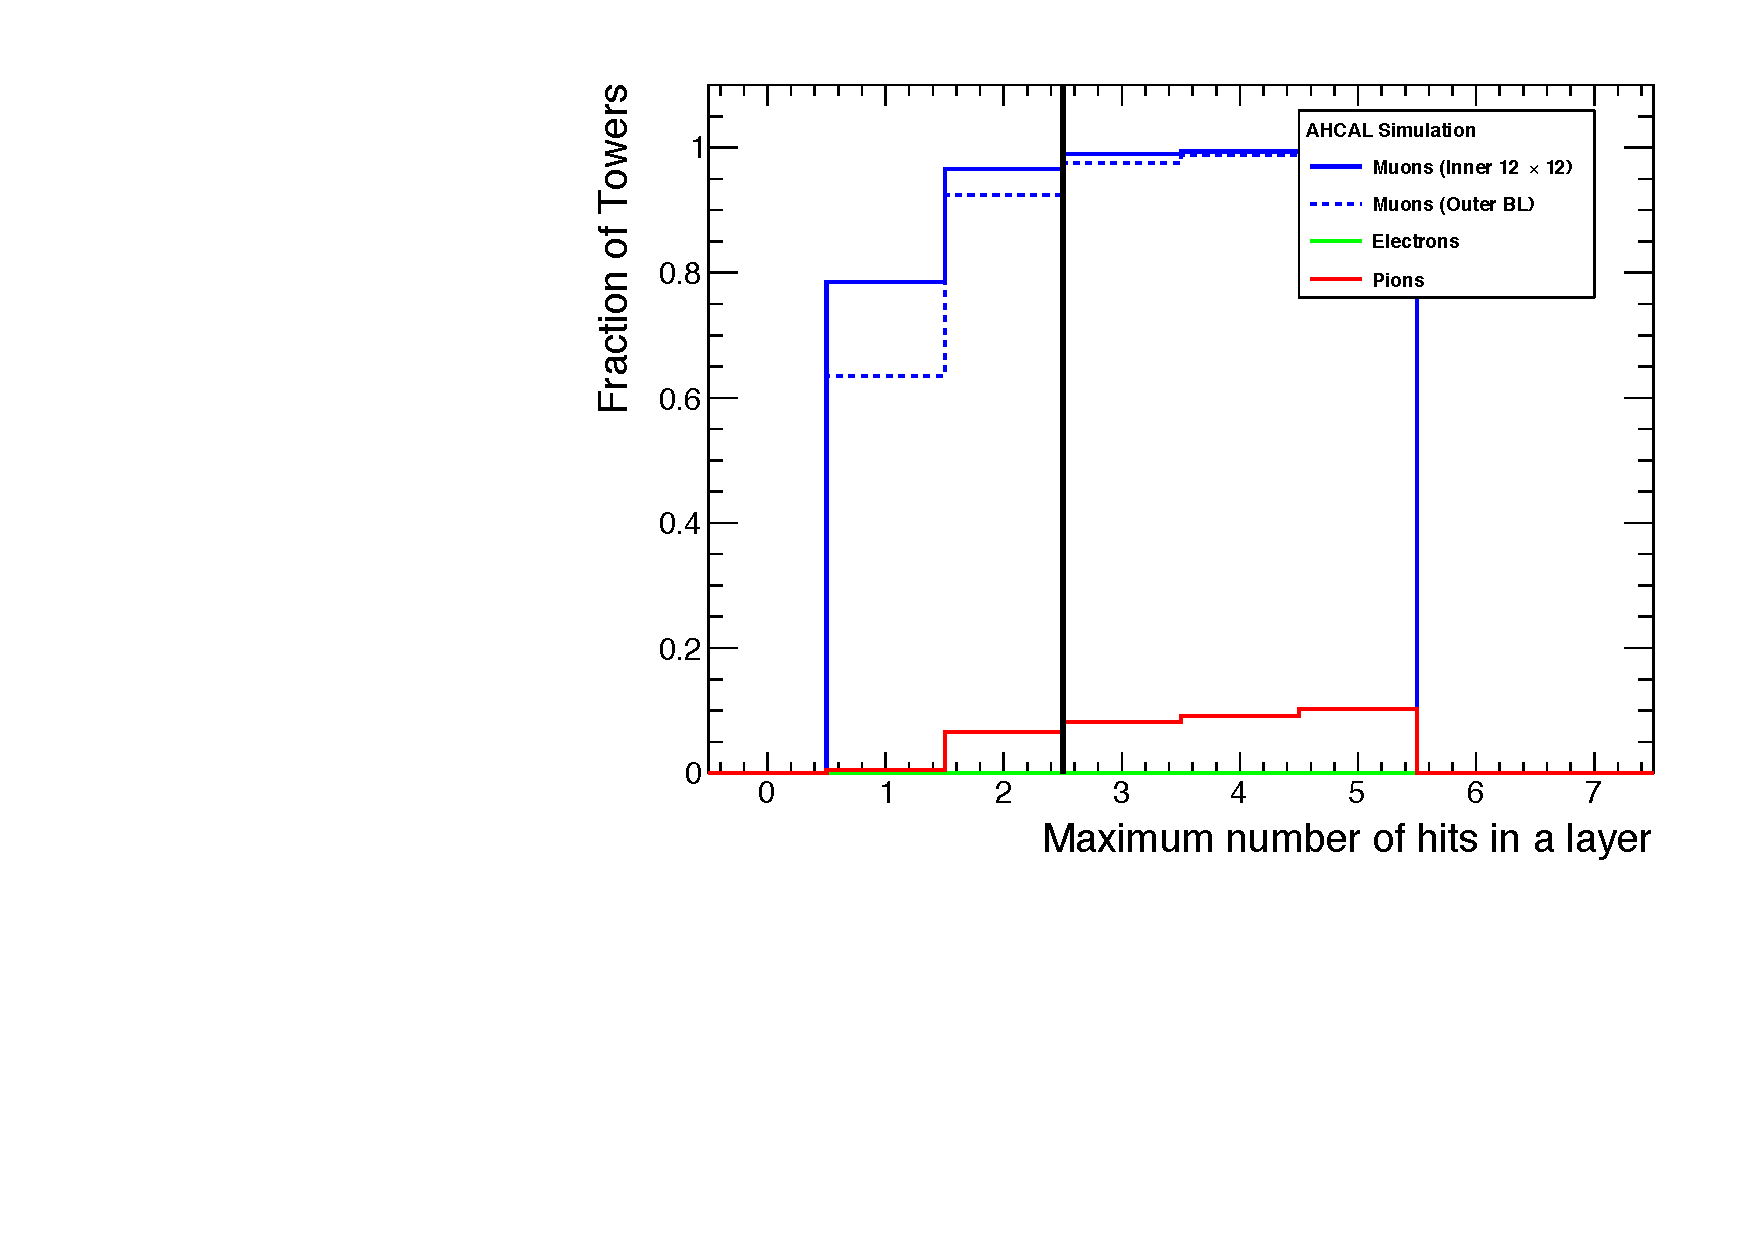
\includegraphics[width=1\linewidth]{chap5/fig_AHCAL_timing/Muons/TrackFinderCut_nHitsLayer_Muons}
		\caption{Maximum number of hits per layer normalized to the number of AHCAL Towers.} \label{fig:Muons_Track_nHitsLayer}
	\end{subfigure}
	\hfill
	\begin{subfigure}[t]{0.5\textwidth}
		\centering
		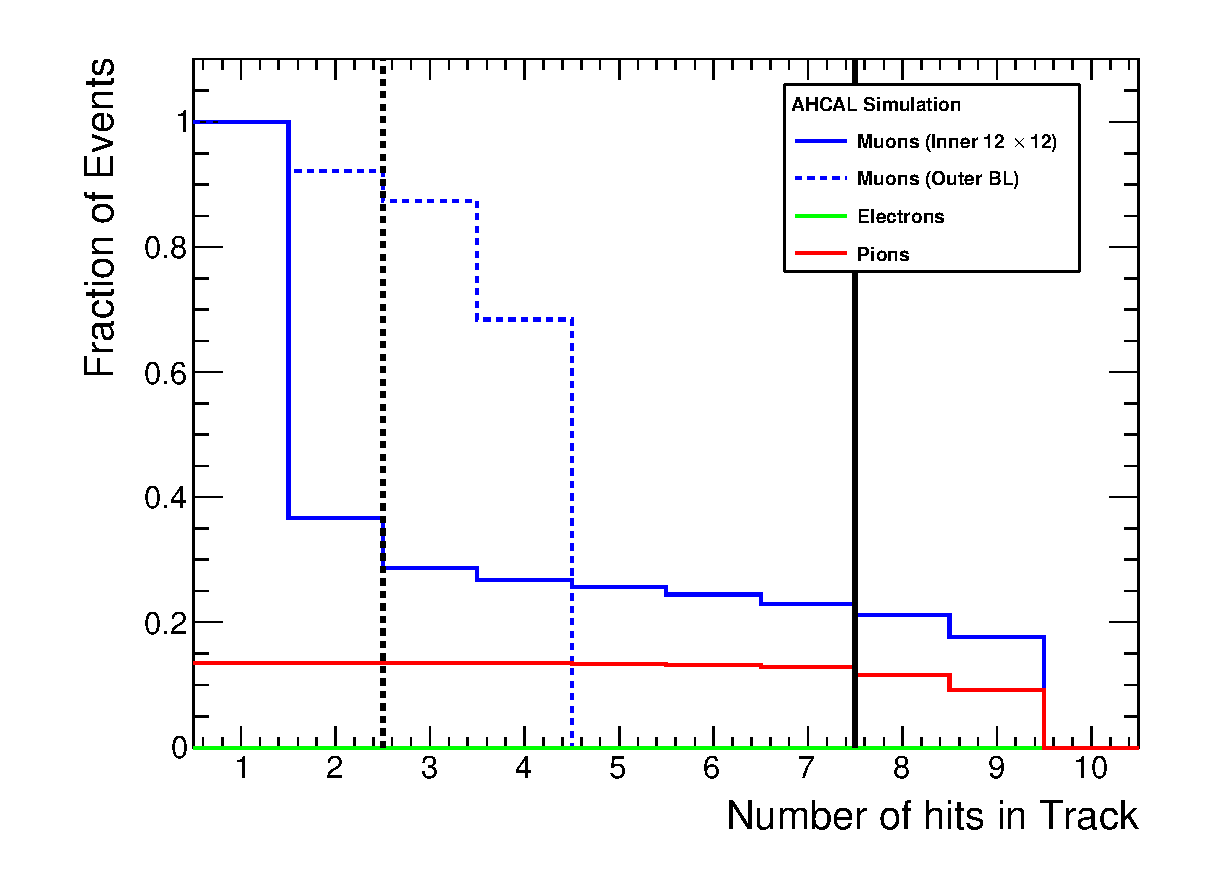
\includegraphics[width=1\linewidth]{chap5/fig_AHCAL_timing/Muons/TrackFinderCut_nHitsTrack_Muons}
		\caption{Number of hits in a track normalized to the number of events.} \label{fig:Muons_Track_nHits}
	\end{subfigure}
	\caption{\subref{fig:Muons_Track_nHitsLayer}) Distribution of the maximum number of hits for simulated muons, electrons and pions at 50 GeV. The black line represents the cut of maximum 2 hits per layer applied for the MIP selection. This cut was done in order to reject late pion showers but avoiding to reject too much of the muons. \subref{fig:Muons_Track_nHits}) Distribution of the number of hits in a track for simulated muons, electrons and pions at 50 GeV. A Tower size of 7 for the inner detector and 2 for the outer big layers was chosen.}
\end{figure}

\subsection{Electron Selection}
\label{subsec:elec_sel}

The electron selection is done to simply extract single electron showers contained in the AHCAL. These events are needed in order to validate the timing behavior in simulation as well as the detector simulation model. For the selection, an \textit{Event Quality} pre-selection is done using the beam instrumentation and layer information. Only events with a Cherenkov tag (only applied on data) are used and as well the energy in the three first layer of the AHCAL ($E_3+E_4+E_5$) must be over 10 MIP. Distributions of the energy in the three first layer of the AHCAL for simulated 10 and 50 GeV muons, electrons and pions can be seen on figures \ref{fig:e10GeV_E3} and \ref{fig:e50GeV_E3}.

In a next step, the electron selection is performed. Due to the number of unusable layers especially the front ECAL layers and the fact that the detector is not fully equipped, an alternative selection needed to be performed to effectively select electrons. As no look into calorimeter linearity and energy resolution is done in this thesis, a cut on the number of hits per event ($n_{Hits}$) versus the center of gravity in z ($CoG_Z < 250 mm$) can be done. This does not induce any bias for a timing analysis, just would only reduce the event statistics.

To ensure a complete containment of the shower and a rejection of possible pion showers, an additional cut on the energy deposited in the last two layers ($(E_{13}+E_{14})/\Sigma E$) is done and must be under 1\% of the energy sum of the event. Distributions of each selection cut are shown in figures \ref{fig:electronselection} for simulated 10 GeV and 50 GeV muons, electrons and pions. Due to the restriction on the number of hits per event, the cuts are energy dependent. Additionally to reduce transverse leakage, the shower center of gravity in X and Y needs to be within $-90 mm$ and $90 mm$.

The selection cuts are summed up in table \ref{table:electron_sel} for each energies. The selection efficiencies between 10 and 50 GeV are shown in table \ref{table:eff_electron} obtained from simulated samples of muons, electrons and pions with QGSP\_BERT\_HP physics list.

\begin{table}[htb!]
	\centering
	\caption{Electron selection efficiency for between 10 and 50 GeV.}
	\label{table:eff_electron}
	\begin{tabular}{@{} llll @{}}
		\hline
		\textbf{Beam Energy} & \textbf{$\epsilon_{\mu}$} & \textbf{$\epsilon_{e}$} & \textbf{$\epsilon_{\pi}$}\\
		\hline
		10 GeV & <0.1\% & 96\% & 15.9\%\\
		15 GeV & <0.1\% & 95.7\% & 10.1\%\\
		20 GeV & <0.1\% & 95.2\% & 6.3\%\\
		30 GeV & <0.1\% & 93.9\% & 2.3\%\\
		40 GeV & <0.1\% & 92.7\% & 1.2\%\\
		50 GeV & <0.1\% & 91.5\% & 1.1\%\\
		\hline
	\end{tabular}
\end{table}

\begin{figure}[htbp!]
	\begin{subfigure}[t]{0.5\textwidth}
		\centering
		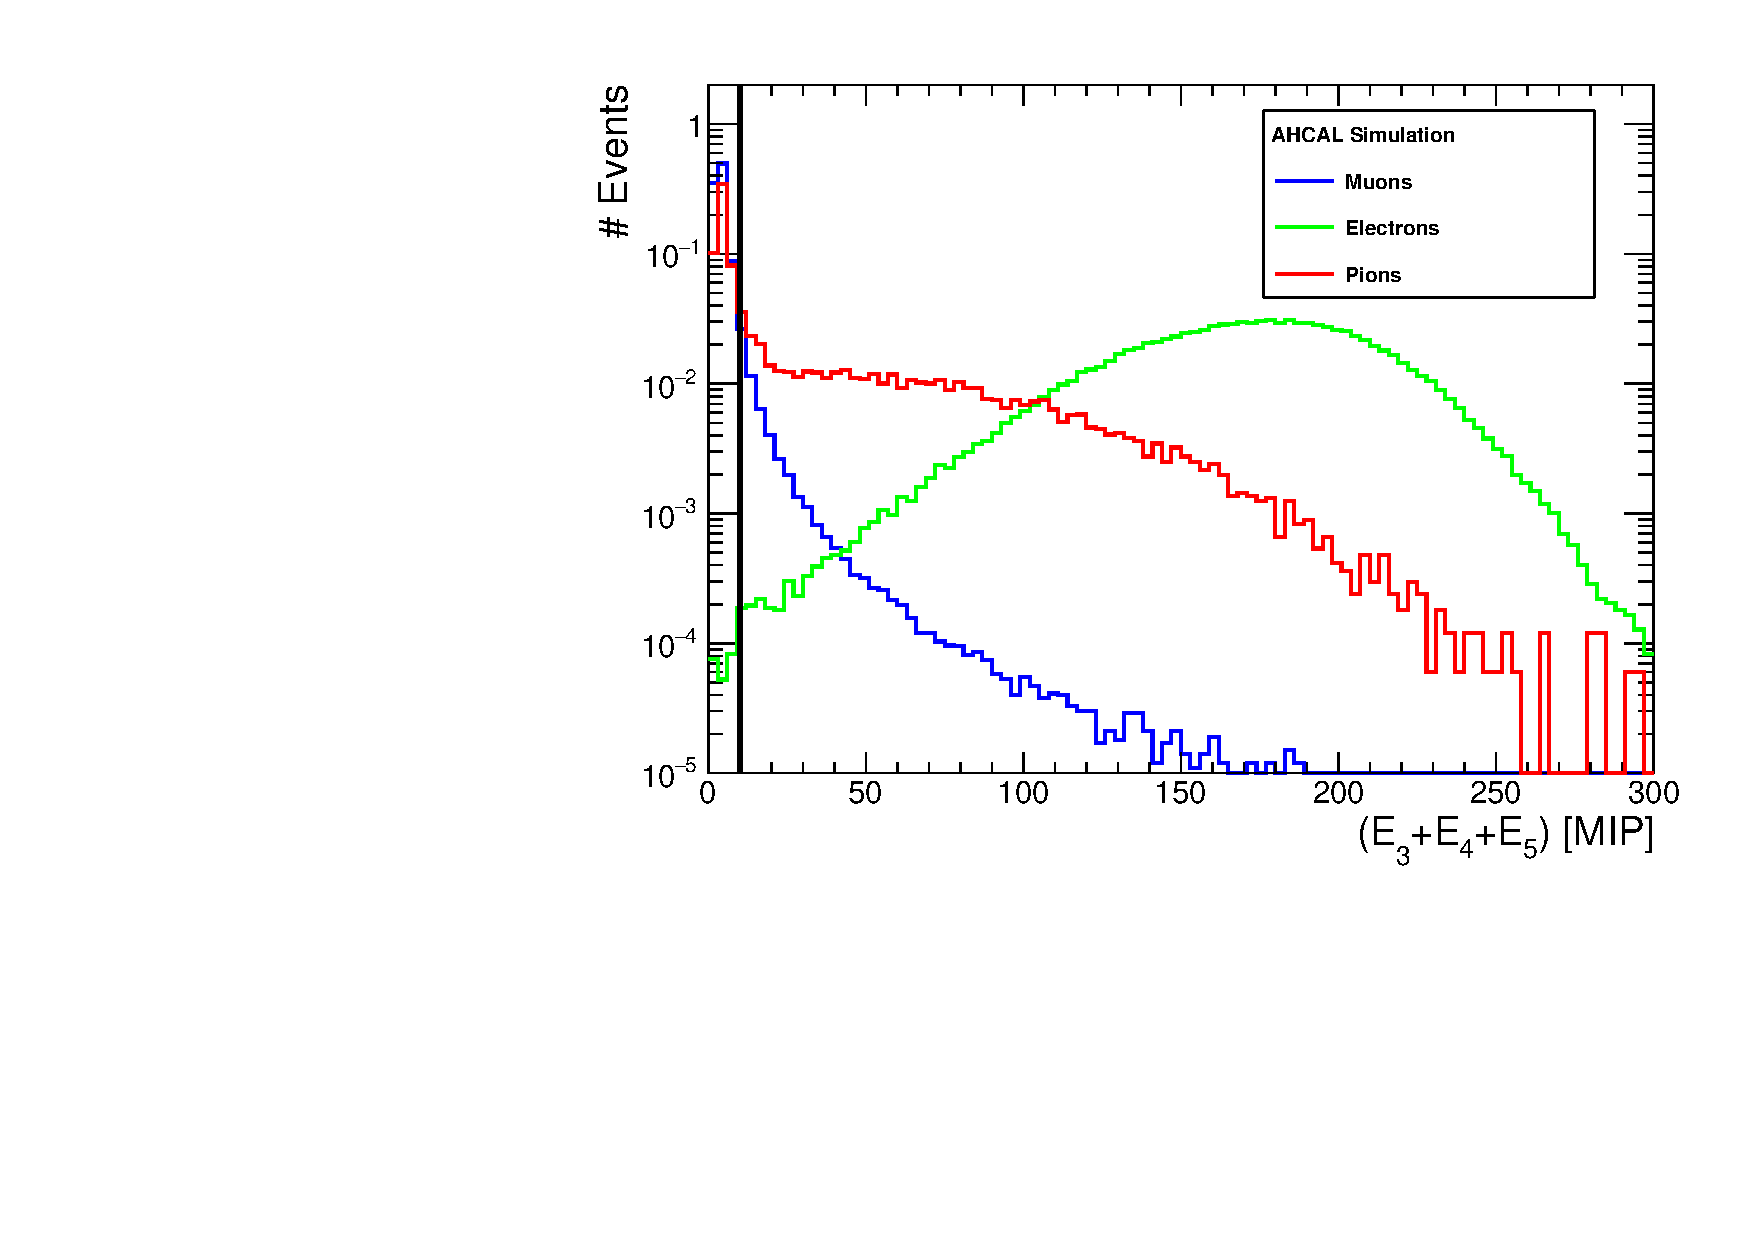
\includegraphics[width=1\linewidth]{chap5/fig_AHCAL_timing/Electrons/SelectionCut_EnergyE3_10GeV}
		\caption{10 GeV.} \label{fig:e10GeV_E3}
	\end{subfigure}
	\hfill
	\begin{subfigure}[t]{0.5\textwidth}
		\centering
		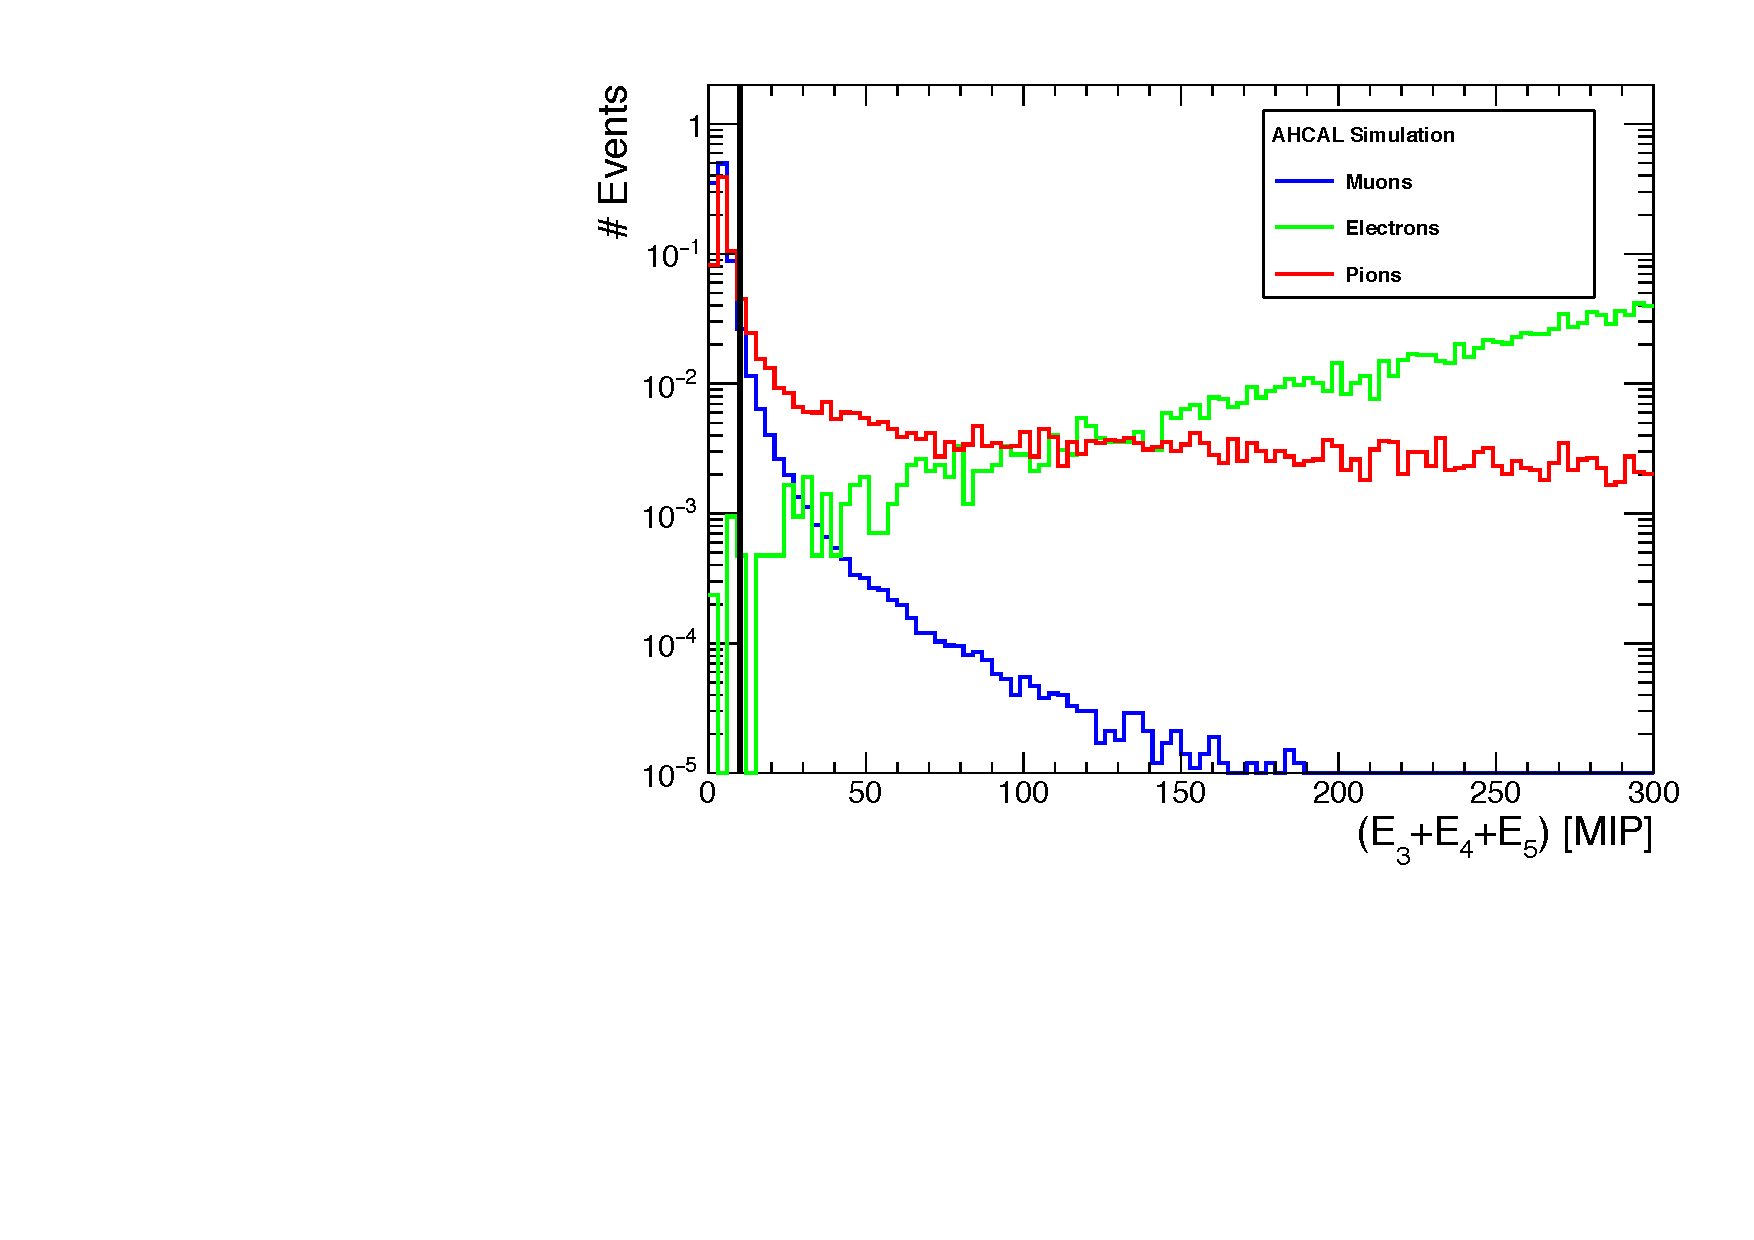
\includegraphics[width=1\linewidth]{chap5/fig_AHCAL_timing/Electrons/SelectionCut_EnergyE3_50GeV}
		\caption{50 GeV.} \label{fig:e50GeV_E3}
	\end{subfigure}
	\hfill
	\begin{subfigure}[t]{0.5\textwidth}
		\centering
		\includegraphics[width=1\linewidth]{chap5/fig_AHCAL_timing/Electrons/SelectionCut_nHitsCoGZ_10GeV}
		\caption{10 GeV.} \label{fig:e10GeV_nHitsCoGZ}
	\end{subfigure}
	\hfill
	\begin{subfigure}[t]{0.5\textwidth}
		\centering
		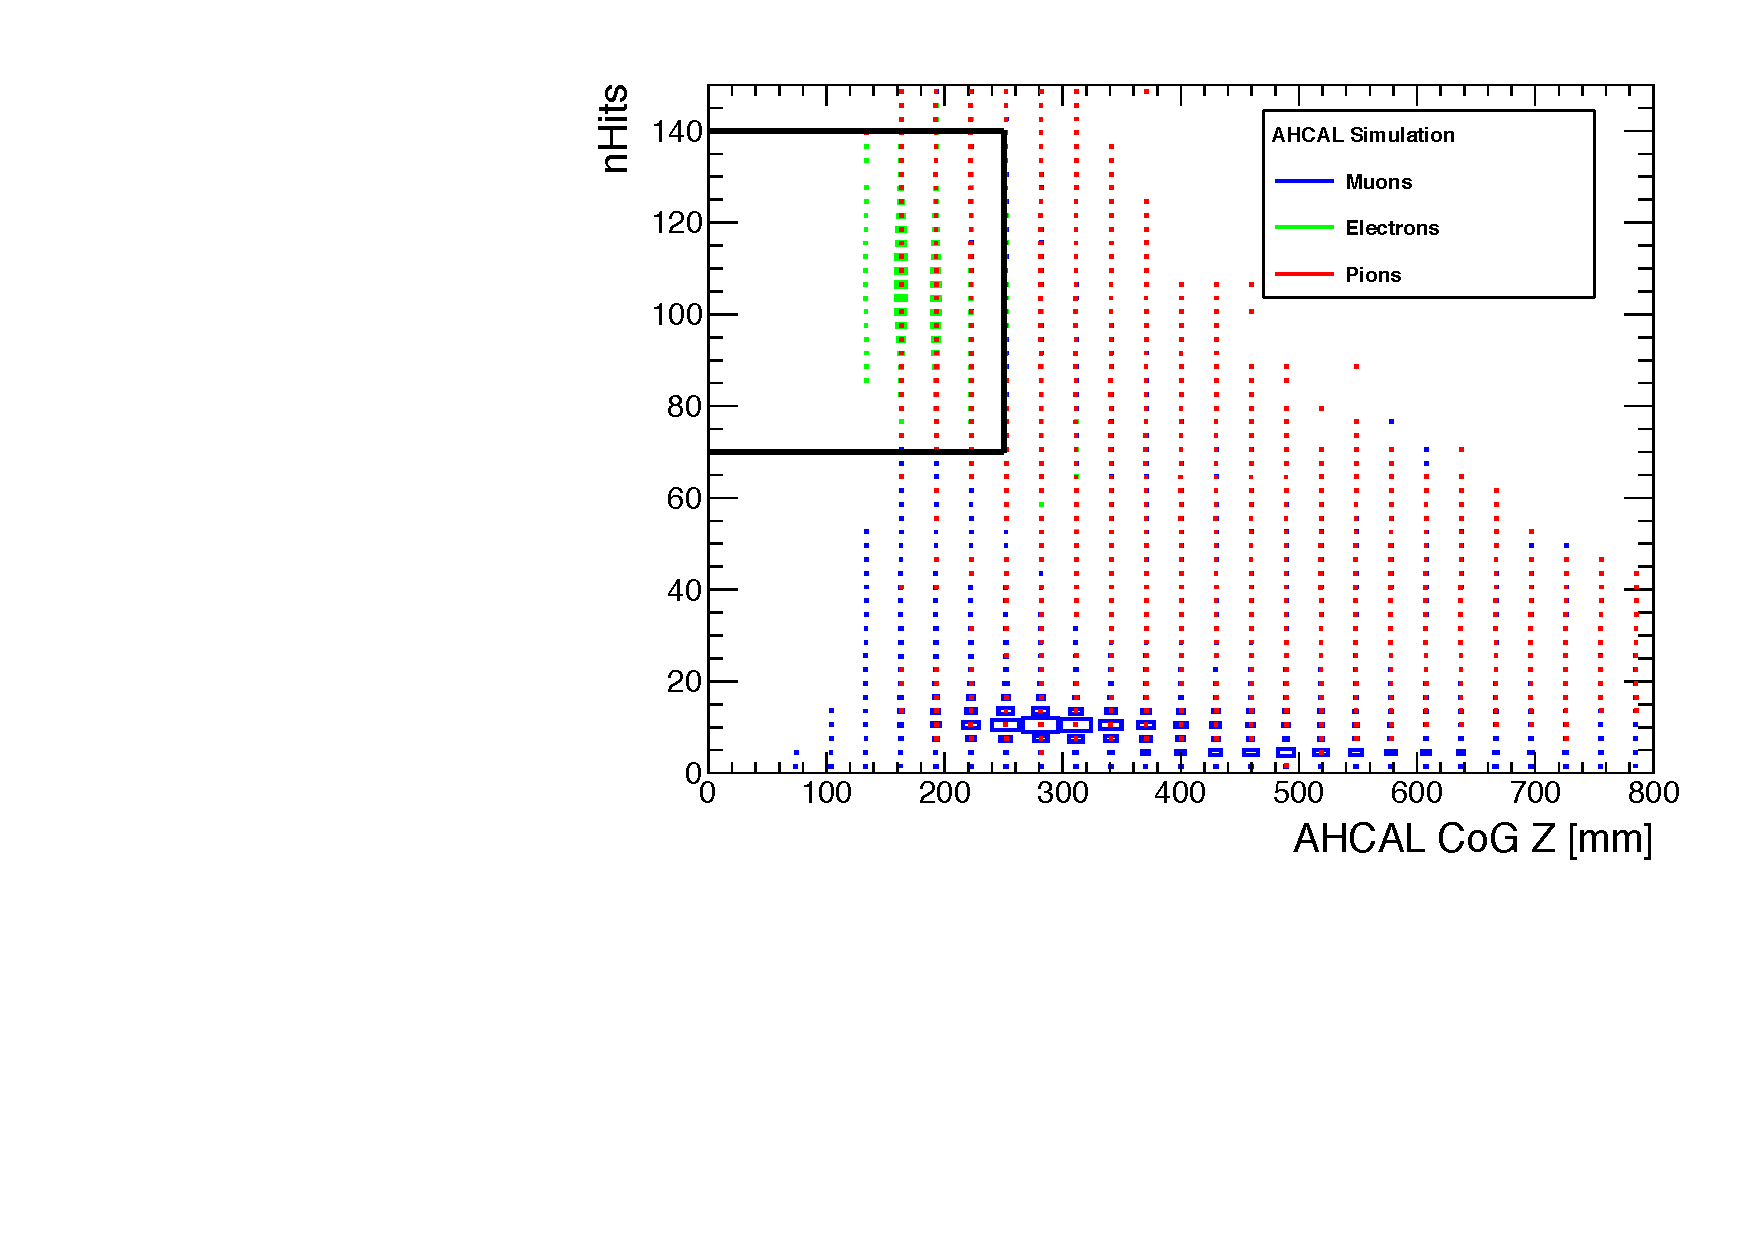
\includegraphics[width=1\linewidth]{chap5/fig_AHCAL_timing/Electrons/SelectionCut_nHitsCoGZ_50GeV}
		\caption{50 GeV.} \label{fig:e50GeV_nHitsCoGZ}
	\end{subfigure}
	\hfill
	\begin{subfigure}[t]{0.5\textwidth}
		\centering
		\includegraphics[width=1\linewidth]{chap5/fig_AHCAL_timing/Electrons/SelectionCut_EnergyLastLayers_10GeV}
		\caption{10 GeV.} \label{fig:e10GeV_Elast}
	\end{subfigure}
	\hfill
	\begin{subfigure}[t]{0.5\textwidth}
		\centering
		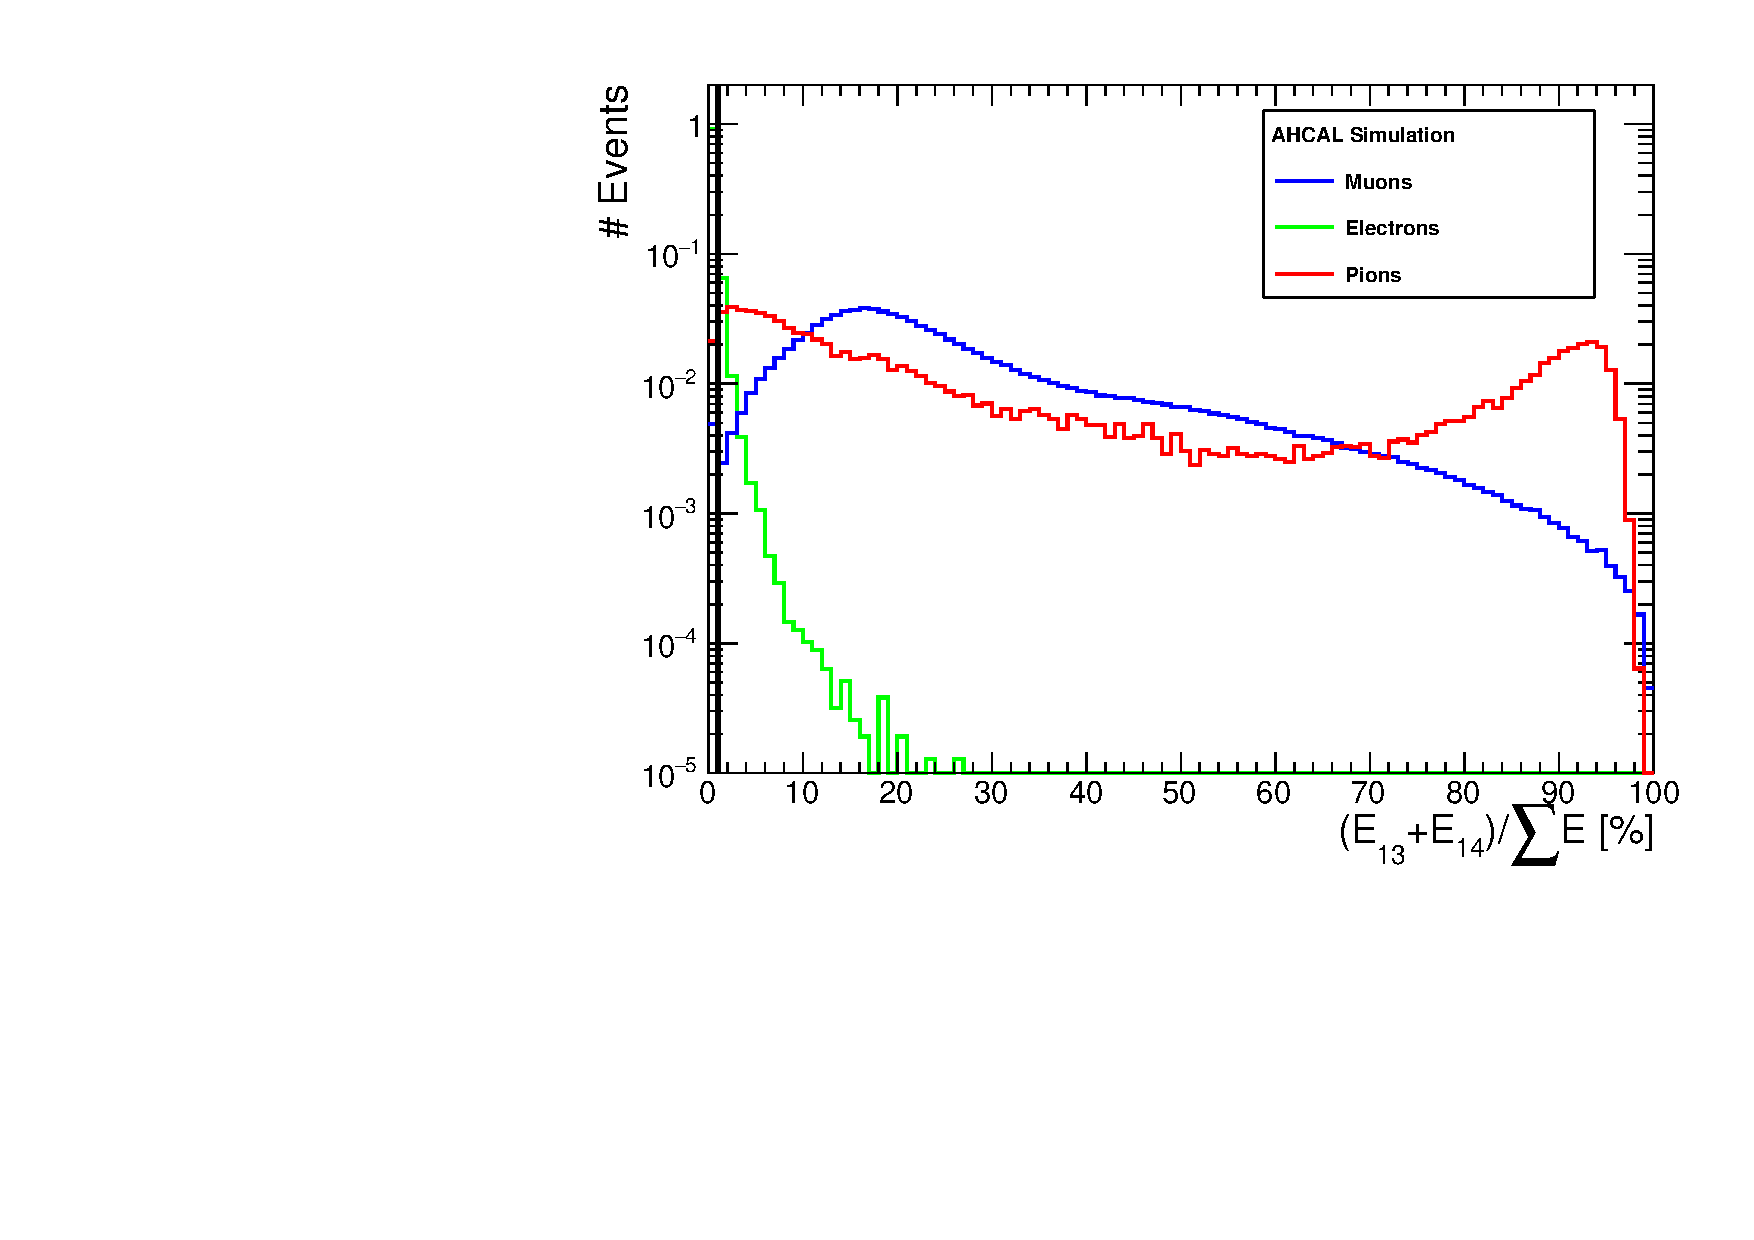
\includegraphics[width=1\linewidth]{chap5/fig_AHCAL_timing/Electrons/SelectionCut_EnergyLastLayers_50GeV}
		\caption{50 GeV.} \label{fig:e50GeV_Elast}
	\end{subfigure}
	\caption{Plots of simulated muon, electron and pion beams between 10 and 50 GeV. Theses plots were used to determine the best selection criterium for electrons.} \label{fig:electronselection}
\end{figure}

\subsection{Pion Selection}

A simple selection is performed on pion events. The goal is to reject punch-through pions, muons and possible electron contamination. The selection is similar as the electron selection. An \textit{Event Quality} pre-selection is performed utilizing the Cherenkov information, events with no Cherenkov ON are selected. This is only applied to data. The pion selection is based on the same variables: $cog_Z:n_{Hits}$ plane, $(E_{13}+E_{14})/\Sigma E$ and additionally the number of hits in two first AHCAL layers ($N_3+N_4$). The number of hits required per event needs to be over 20 to reject most muons or punch-through pions without cutting on the center of gravity in z in order not to bias the selection on the start of the pion shower. To ensure that the pion showered, the energy in the last two layers of the AHCAL must be over 1\%. And finally, to mitigate possible particle contamination from electrons, the number of hits in the two first AHCAL layer must be under 5. The distributions of each selection cut are shown in figures \ref{fig:pionselection} for simulated 10 GeV and 90 GeV muons, electrons and pions.

Moreover, after a long investigation, multiple particle events were observed in the data. As no beam instrumentation could be utilized for rejecting these events, a simple rejection method based on time clusters was developed. All hits per event are placed and ordered in time in a vector. For each hits after 50 ns, a window of 30 ns is looked after and the number of hits in that window is counted. If the number of hits is over 5, it is counted as a late cluster. The event is rejected if the number of late clusters is over zero. This method was based on data in order to remove efficiently multi-particle events. The multi particle event rejection has been checked on simulated data and affects the selection between <0.1\% up to 2\% from 10 to 90 GeV pions.
These multi-particle events are greatly suppressed in data using this method but due to the calorimeter not being fully equipped, some contimination may remain in the data.

A detailed description of the selection cuts are shown in table \ref{table:pion_sel}.

\begin{table}[htb!]
	\centering
	\caption{Pion selection efficiency between 10 and 90 GeV.}
	\label{table:eff_electron}
	\begin{tabular}{@{} llll @{}}
		\hline
		\textbf{Beam Energy} & \textbf{$\epsilon_{\mu}$} & \textbf{$\epsilon_{e}$} & \textbf{$\epsilon_{\pi}$}\\
		\hline
		10 GeV & <0.1\% & <0.1\% & 29.9\%\\
		30 GeV & 0.9\% & <0.1\% & 50.3\%\\
		50 GeV & 0.9\% & <0.1\% & 51.1\%\\
		70 GeV & 0.9\% & <0.1\% & 51\%\\
		90 GeV & 0.9\% & <0.1\% & 50.2\%\\
		\hline
	\end{tabular}
\end{table}

\begin{figure}[htbp!]
	\begin{subfigure}[t]{0.5\textwidth}
		\centering
		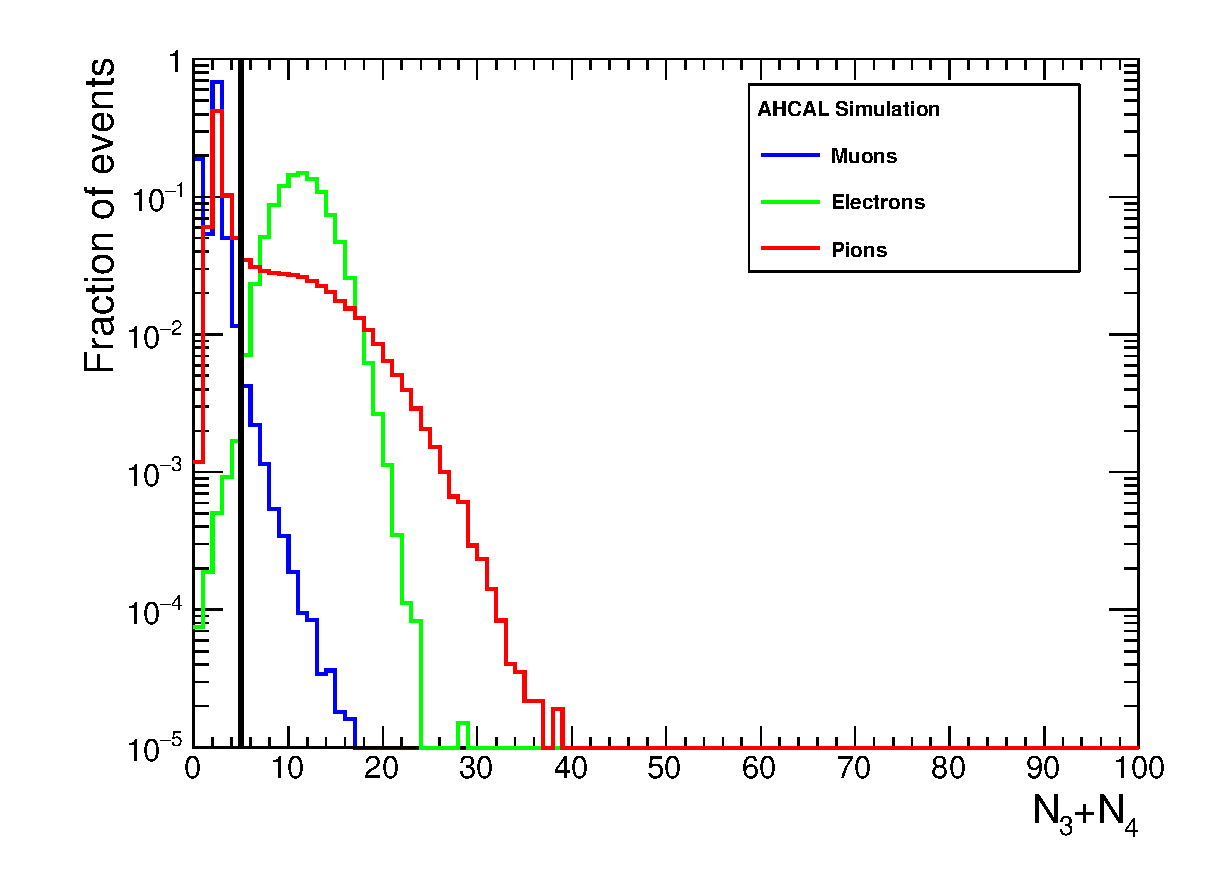
\includegraphics[width=1\linewidth]{chap5/fig_AHCAL_timing/Pions/SelectionCut_N3N4_10GeV}
		\caption{10 GeV.} \label{fig:pi10GeV_N3N4}
	\end{subfigure}
	\hfill
	\begin{subfigure}[t]{0.5\textwidth}
		\centering
		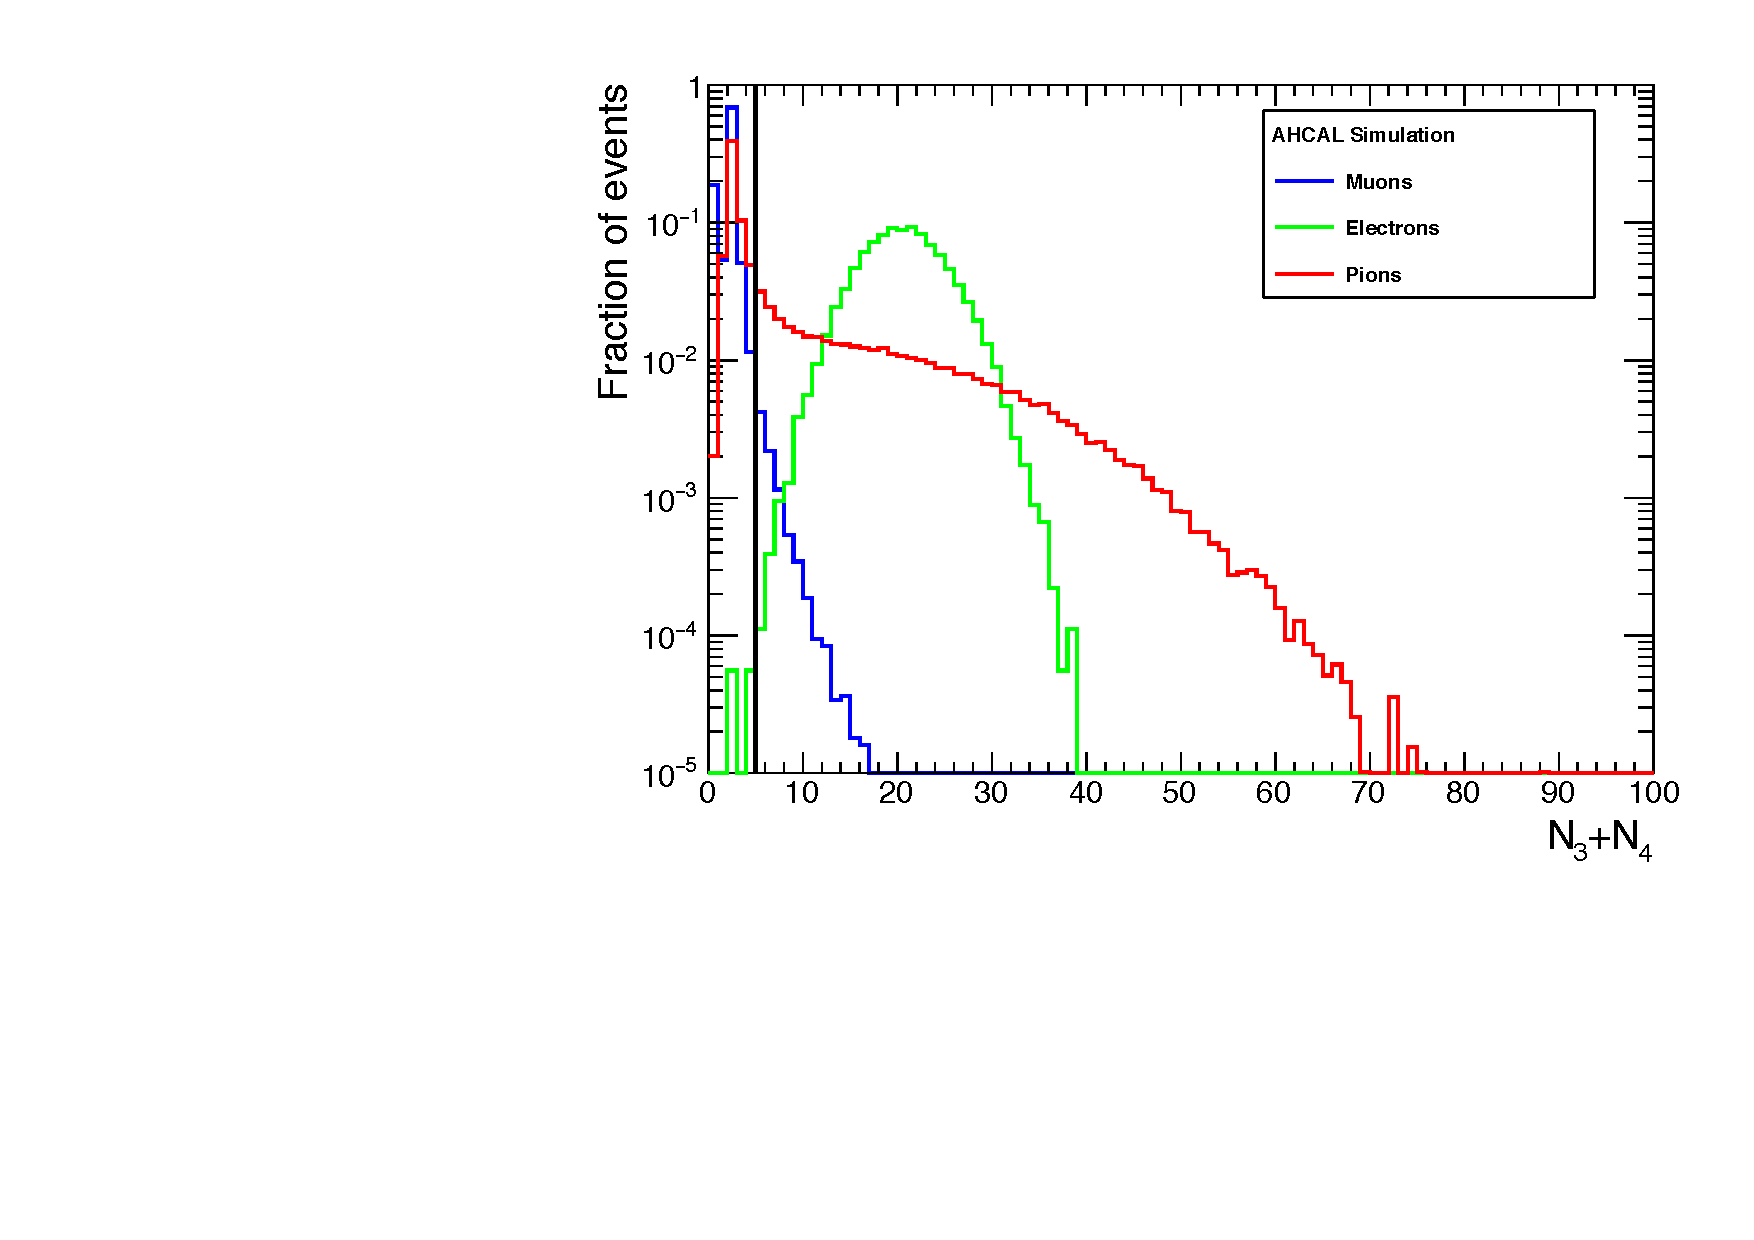
\includegraphics[width=1\linewidth]{chap5/fig_AHCAL_timing/Pions/SelectionCut_N3N4_90GeV}
		\caption{90 GeV.} \label{fig:pi90GeV_N3N4}
	\end{subfigure}
	\hfill
	\begin{subfigure}[t]{0.5\textwidth}
		\centering
		\includegraphics[width=1\linewidth]{chap5/fig_AHCAL_timing/Pions/SelectionCut_nHitsCoGZ_10GeV}
		\caption{10 GeV.} \label{fig:pi10GeV_nHitsCoGZ}
	\end{subfigure}
	\hfill
	\begin{subfigure}[t]{0.5\textwidth}
		\centering
		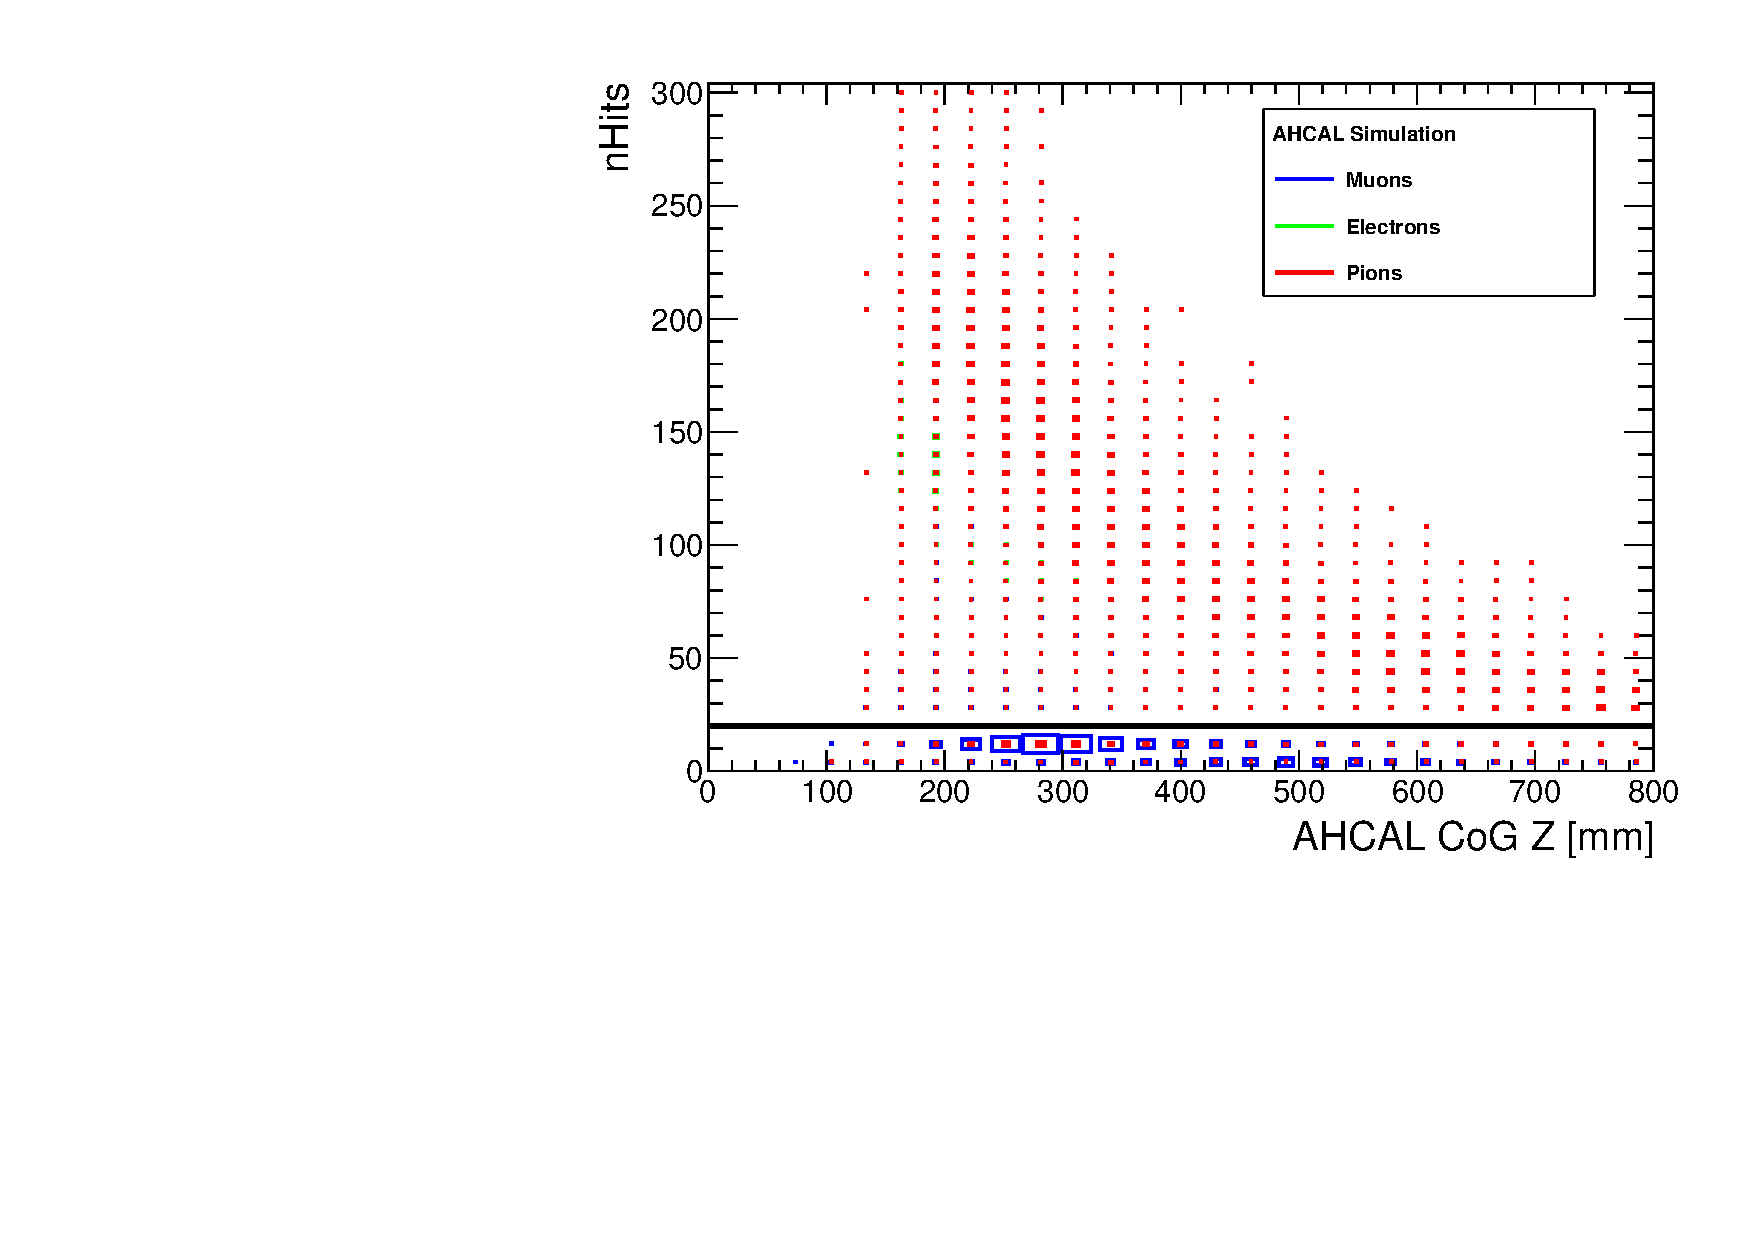
\includegraphics[width=1\linewidth]{chap5/fig_AHCAL_timing/Pions/SelectionCut_nHitsCoGZ_90GeV}
		\caption{90 GeV.} \label{fig:pi90GeV_nHitsCoGZ}
	\end{subfigure}
	\hfill
	\begin{subfigure}[t]{0.5\textwidth}
		\centering
		\includegraphics[width=1\linewidth]{chap5/fig_AHCAL_timing/Pions/SelectionCut_EnergyLastLayers_10GeV}
		\caption{10 GeV.} \label{fig:pi10GeV_Elast}
	\end{subfigure}
	\hfill
	\begin{subfigure}[t]{0.5\textwidth}
		\centering
		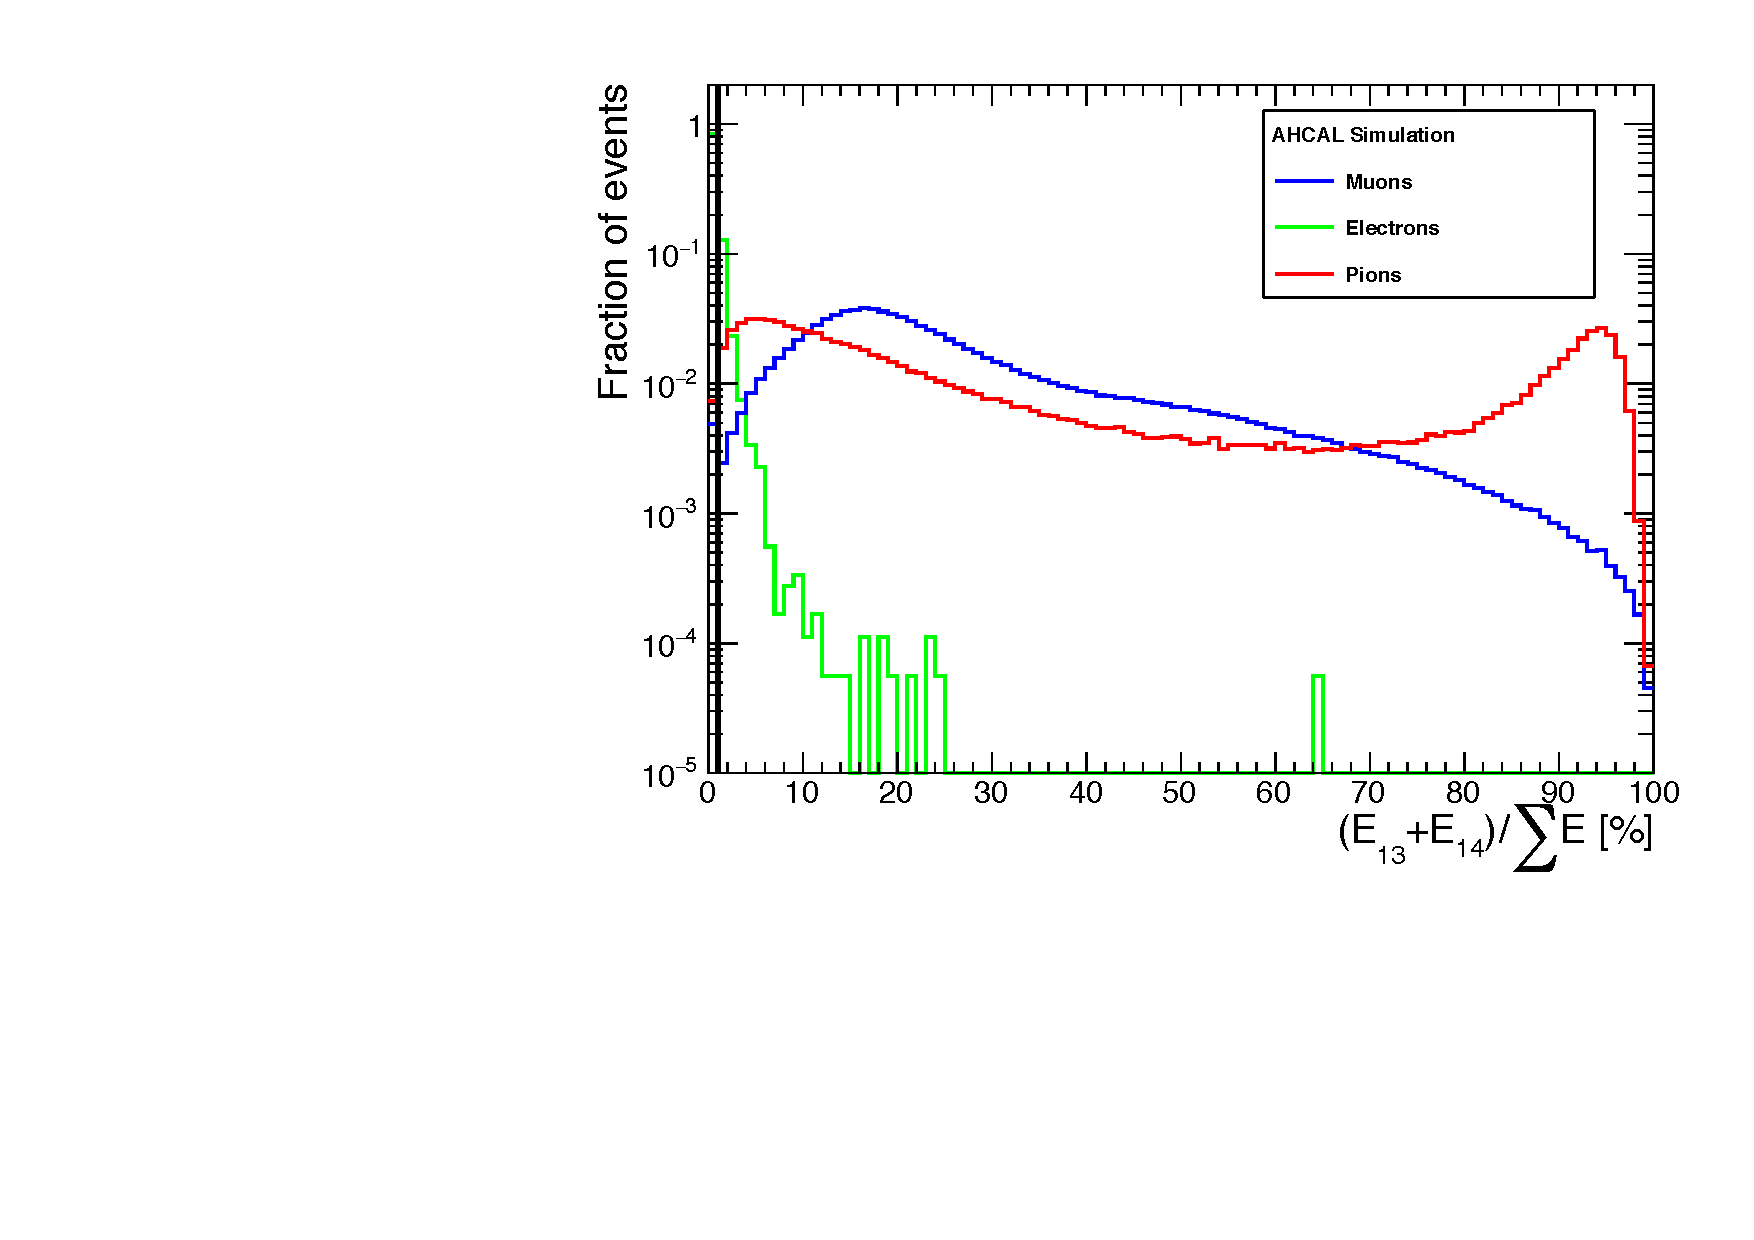
\includegraphics[width=1\linewidth]{chap5/fig_AHCAL_timing/Pions/SelectionCut_EnergyLastLayers_90GeV}
		\caption{90 GeV.} \label{fig:pi90GeV_Elast}
	\end{subfigure}
	\caption{Plots of simulated muon, electron and pion beams between 10 and 90 GeV. Theses plots were used to determine the best selection criterium for pions.} \label{fig:pionselection}
\end{figure}

\subsection{Chip rejection}

For each type of data analysed, a carefull check of each chip has been performed. For all the data collected, the layer 11 is rejected. For the muon data, only a single chip (157) shows a strange behavior likely because the IDACs on this chip were broken.

For the electron data, a relative fraction of hits $r$ following the equation \ref{eq:fraction_rejection} was looked at. If this fraction $r$ is below 98\%, the chip is rejected. This means that most of the hits in the event are in the core of the distribution between -50 and 50 ns. With this method, 20 chips are rejected.

\begin{equation} \label{eq:fraction_rejection}
	r = \frac{1}{N} \left|\int_{50 ns}^{200 ns} \frac{dN(t)}{dt} dt - \int_{-200 ns}^{50 ns} \frac{dN(t)}{dt} dt\right|
\end{equation}

For the pion data, applying the same method as for electrons is not possible due to the late tail related to delayed energy deposition from neutrons. The same chips as for electrons were rejected but additionally, each chip time distribution after correction were maually checked and chips presenting an anormal shape were discarded. This way additionally 16 chips are rejected. This leaves 44 chips in the pion analysis. A detailled table of the rejected chips can be seen in appendix \ref{appendix:rejection}.

\section{Timing Calibration}

\begin{table}[htb!]
	\centering
	\caption{Table with the run statistic before and after selection used for timing calibration.}
	\label{table:mu_elec_runs}
	\resizebox{0.8\textwidth}{!}{%
	\begin{tabular}{@{} llllll @{}}
		\hline
		Runs & Energy & Particle Type & Events (Raw) & Events (sel.) & $\frac{\text{N$_{sel.}$}}{\text{N$_{raw}$}}$ \\
		\hline
		24016-24663 & 50-150 GeV & $\mu^-$ & 1851536 & 836796 & 45.2\% \\
		24528-24577 & 10 GeV & $e^-$ & 268275 & 216656 & 80.8\% \\
		24510-24520 & 15 GeV & $e^-$ & 108092 & 90395 & 83.6\% \\
		24486-24504 & 20 GeV & $e^-$ & 130232 & 110161 & 84.6\% \\
		24460-24470 & 30 GeV & $e^-$ & 82202 & 69692 & 84.8\% \\
		24427-24435 & 40 GeV & $e^-$ & 65901 & 55660 & 84.5\% \\
		24405-24419 & 50 GeV & $e^-$ & 123422 & 104030 & 84.3\% \\
		\hline
	\end{tabular}
	}
\end{table}

To perform the timing calibration of the AHCAL, the complete muon dataset is used. The electron dataset is used in a next step to validate the calibration procedure as described in subsection \ref{subsec:validation} before studying hadronic showers. Table \ref{table:mu_elec_runs} summarizes the runs and datasets used. Raw events are considered if the reference signals T$_{12}$,  T$_{13}$ and T$_{14}$ are present in the event. Selected events are counted after the selection on the error of the time reference as explained in \ref{subsection:time_ref}.

\subsection{Slope calibration}
\label{subsec:slope_calib}

The data analysis is performed in several steps. The first step is the calibration of the time provided by the \textit{SPIROC2B} chip. To reconstruct the time of the first hit in a channel (only a single hit per channel is registered during a bunch-crossing), the TDC value measured needs to be converted into nanoseconds. The value is converted using the following equations:

\begin{equation} \label{eq:slope}
	\text{slope}_{chip, BXID} \: \text{[ns/TDC]} = \frac{3920 \: \text{ns}}{\text{Max}_{chip, BXID} - \text{Pedestal}_{chip, BXID}}
\end{equation}
\begin{equation} \label{eq:time_chn}
	\text{T}_{chn} \: \text{[ns]} = \text{slope}_{chip, BXID} \times (\text{TDC} - \text{Pedestal}_{mem=1} )
\end{equation}

The determination of the parameter $\text{slope}_{chip, BXID}$ is assuming that the TDC ramp in the chip is linear to a first order. The parameters Max$_{chip, BXID}$ and Pedestal$_{chip, BXID}$ in eq.\ref{eq:slope} are extracted from the TDC spectrum for a specific chip and BXID using only the first memory cell as illustrated in figure \ref{fig:TDC_Spectrum}. At the same time, the parameter Pedestal$_{mem=1}$ in eq.\ref{eq:time_chn} is extracted from the spectrum for each channel and the first memory cell of a chip without taking into account the BXID of the ramp as the difference between both pedestal can be corrected for at a later stage. This is accounting for a total of 208 slopes and 3744 pedestals to be extracted for the testbeam setup.

\begin{figure}[htbp!]
	\begin{subfigure}[t]{0.5\textwidth}
		\centering
		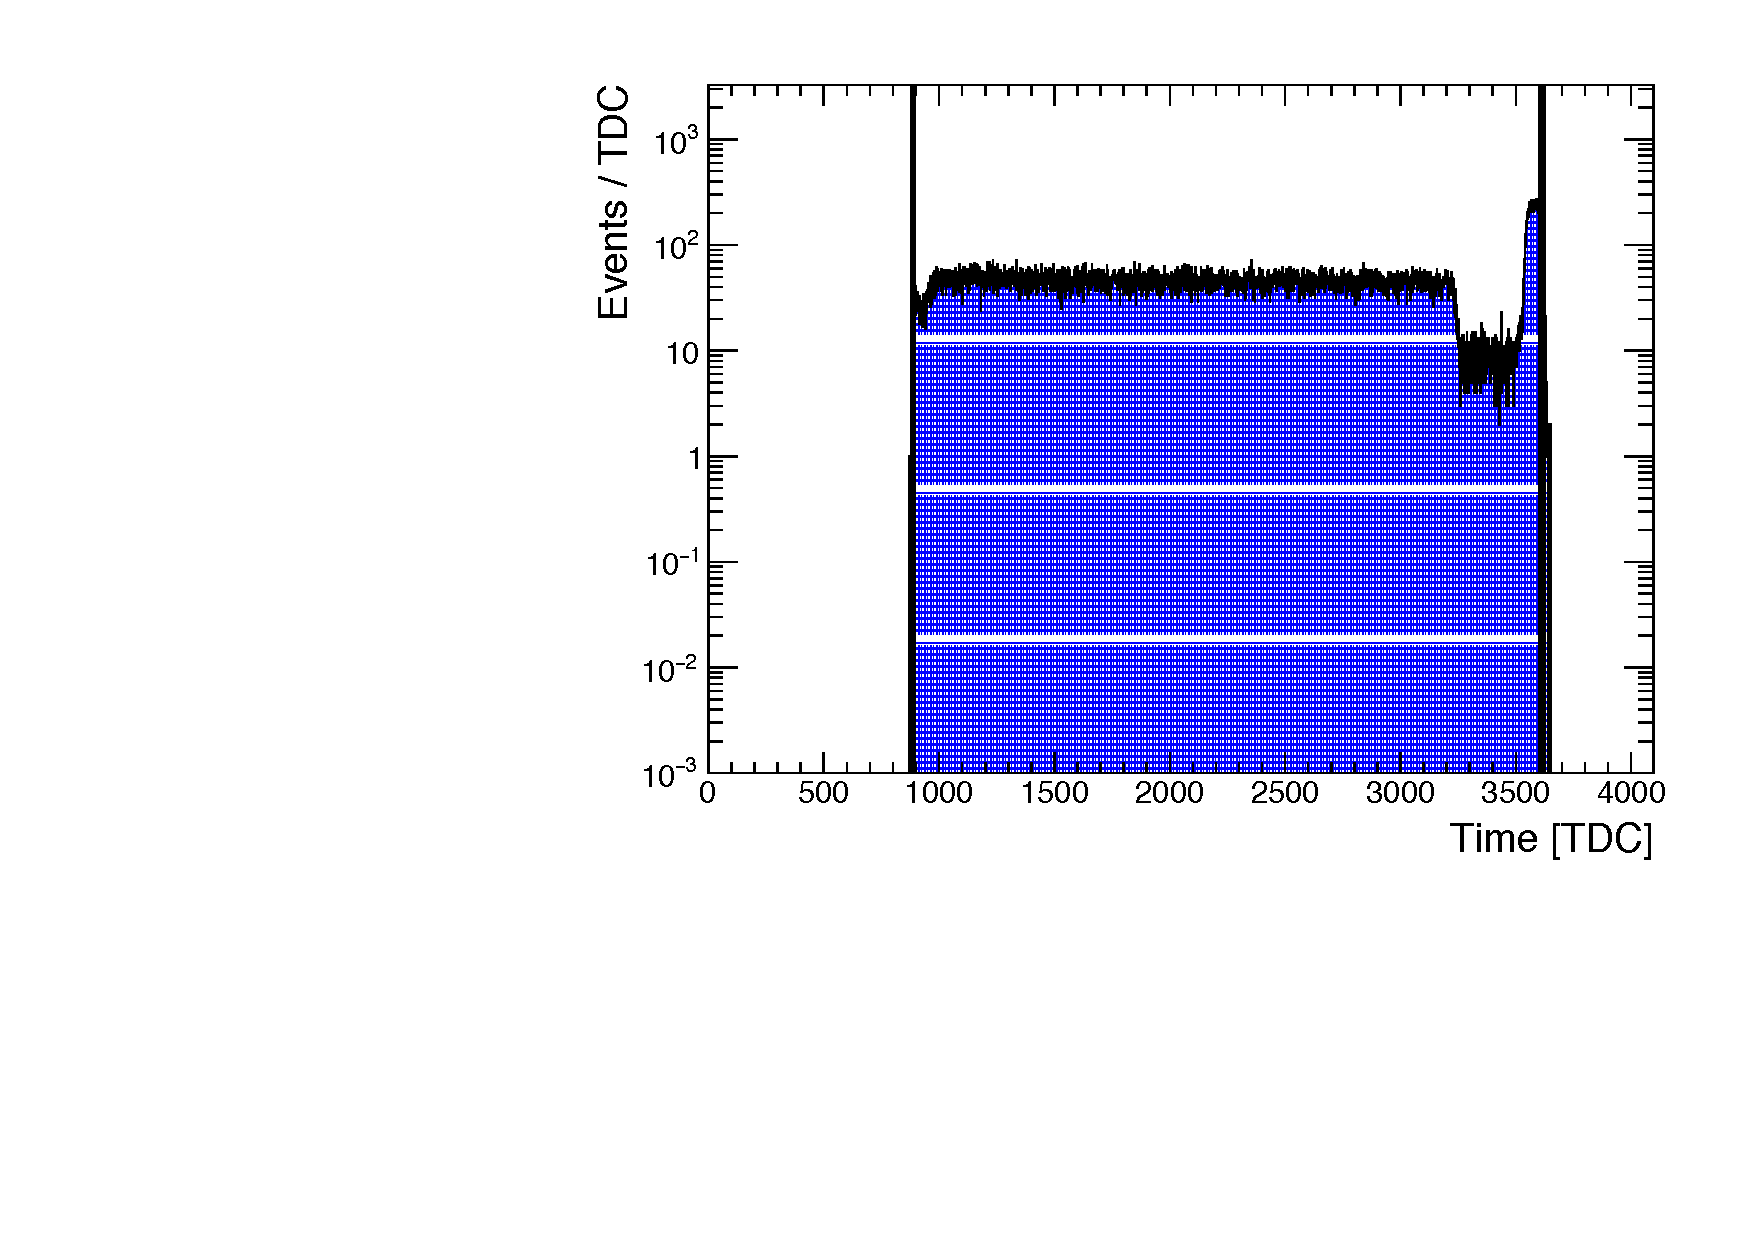
\includegraphics[width=1\linewidth]{chap5/fig_AHCAL_timing/Muons/ExampleTDCSpectra}
		\caption{TDC Spectrum of a typical chip.} \label{fig:TDC_Spectrum}
	\end{subfigure}
	\hfill
	\begin{subfigure}[t]{0.5\textwidth}
		\centering
		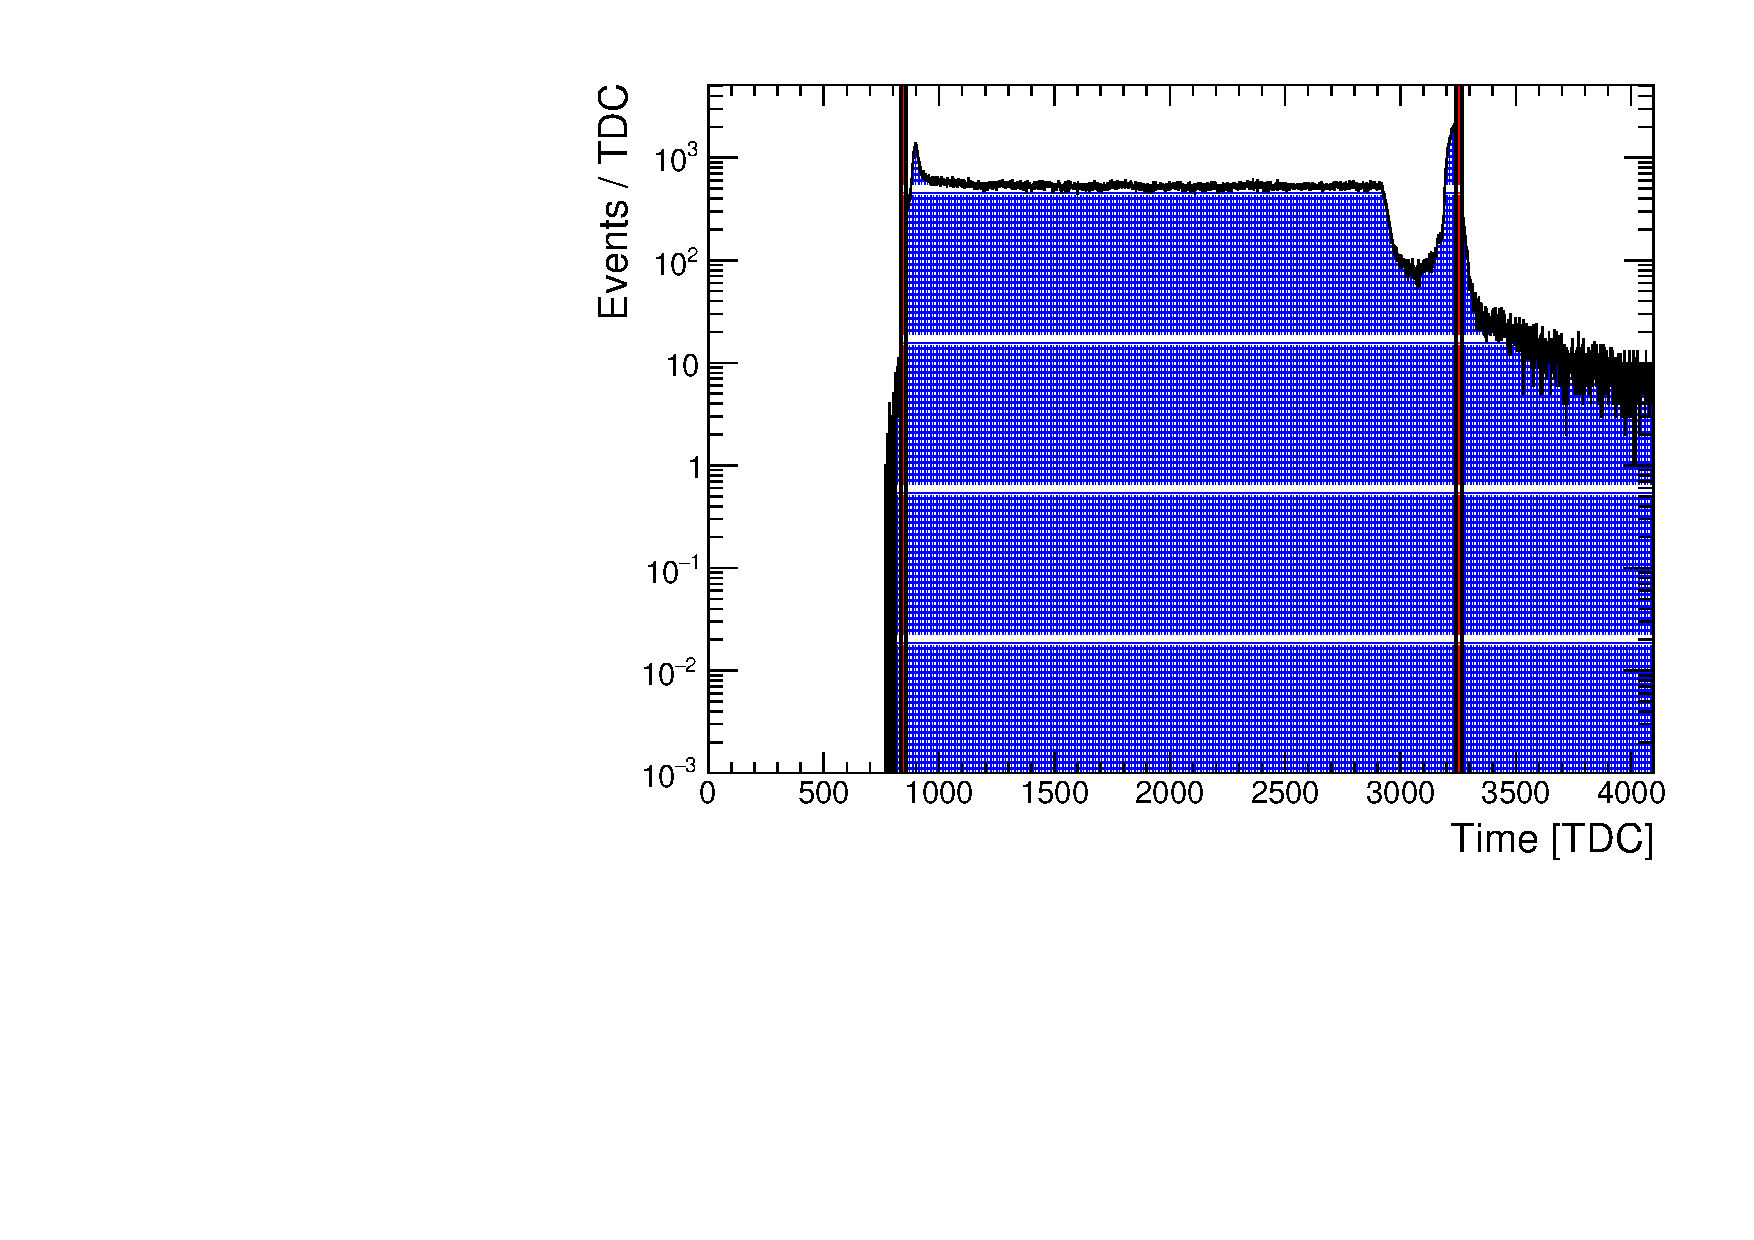
\includegraphics[width=1\linewidth]{chap5/fig_AHCAL_timing/Muons/BadTDCSpectra_Layer12}
		\caption{TDC Spectrum of a bad chip.} \label{fig:TDC_Spectrum_bad}
	\end{subfigure}
	\caption{\subref{fig:TDC_Spectrum}) The red rectangle are the fitted Max and Pedestal parameters for this chip. The yellow bands represents estimation of the error made on the extraction of the parameters by a variation of 1 RMS of the threshold $\mu$. The parameters extracted are slope = 1.56 $\pm$ 0.01, Pedestal = 816 $\pm$ 9 and Maximum = 3336 $\pm$ 8. \subref{fig:TDC_Spectrum_bad}) An example of a bad chip presenting a long tail to high TDC values. The reason is not totally understood but present on all chips on that layer.}
\end{figure}

The technique of extraction is based on an edge detection method. For each chip and BXID, an histogram is filled with the y value of each bin then the mean of this histogram is defined as a threshold $\mu$. The parameter Pedestal$_{chip, BXID}$ is extracted as the first bin above 30\% of $\mu$. For the parameter Max$_{chip, BXID}$, it is extracted by taking 50\% of the maximum bin of the original histogram. The maximum seems not to be exactly at the last bin of the spectrum, this is due to the technique that needed to be robust against strange spectra as shown in figure \ref{fig:TDC_Spectrum_bad}.

An estimation of the errors made on the pedestal and maximum is done by looking at the maximum difference between 1 RMS of $\mu$ and 33\% of the maximum bin to the extracted value and are represented on the spectra by the yellow bands. More details about the estimation of the calibration errors is described in the appendix \ref{appendix:calib_error}.

The extracted values for the slopes are in the expected range of 1.6 ns per TDC bin due to the limited dynamic range provided by the chip (around 2500 bins for 4 $\mu$s) which is in aggreement with figure \ref{fig:slope_time}.

\begin{figure}[htbp!]
	\centering
	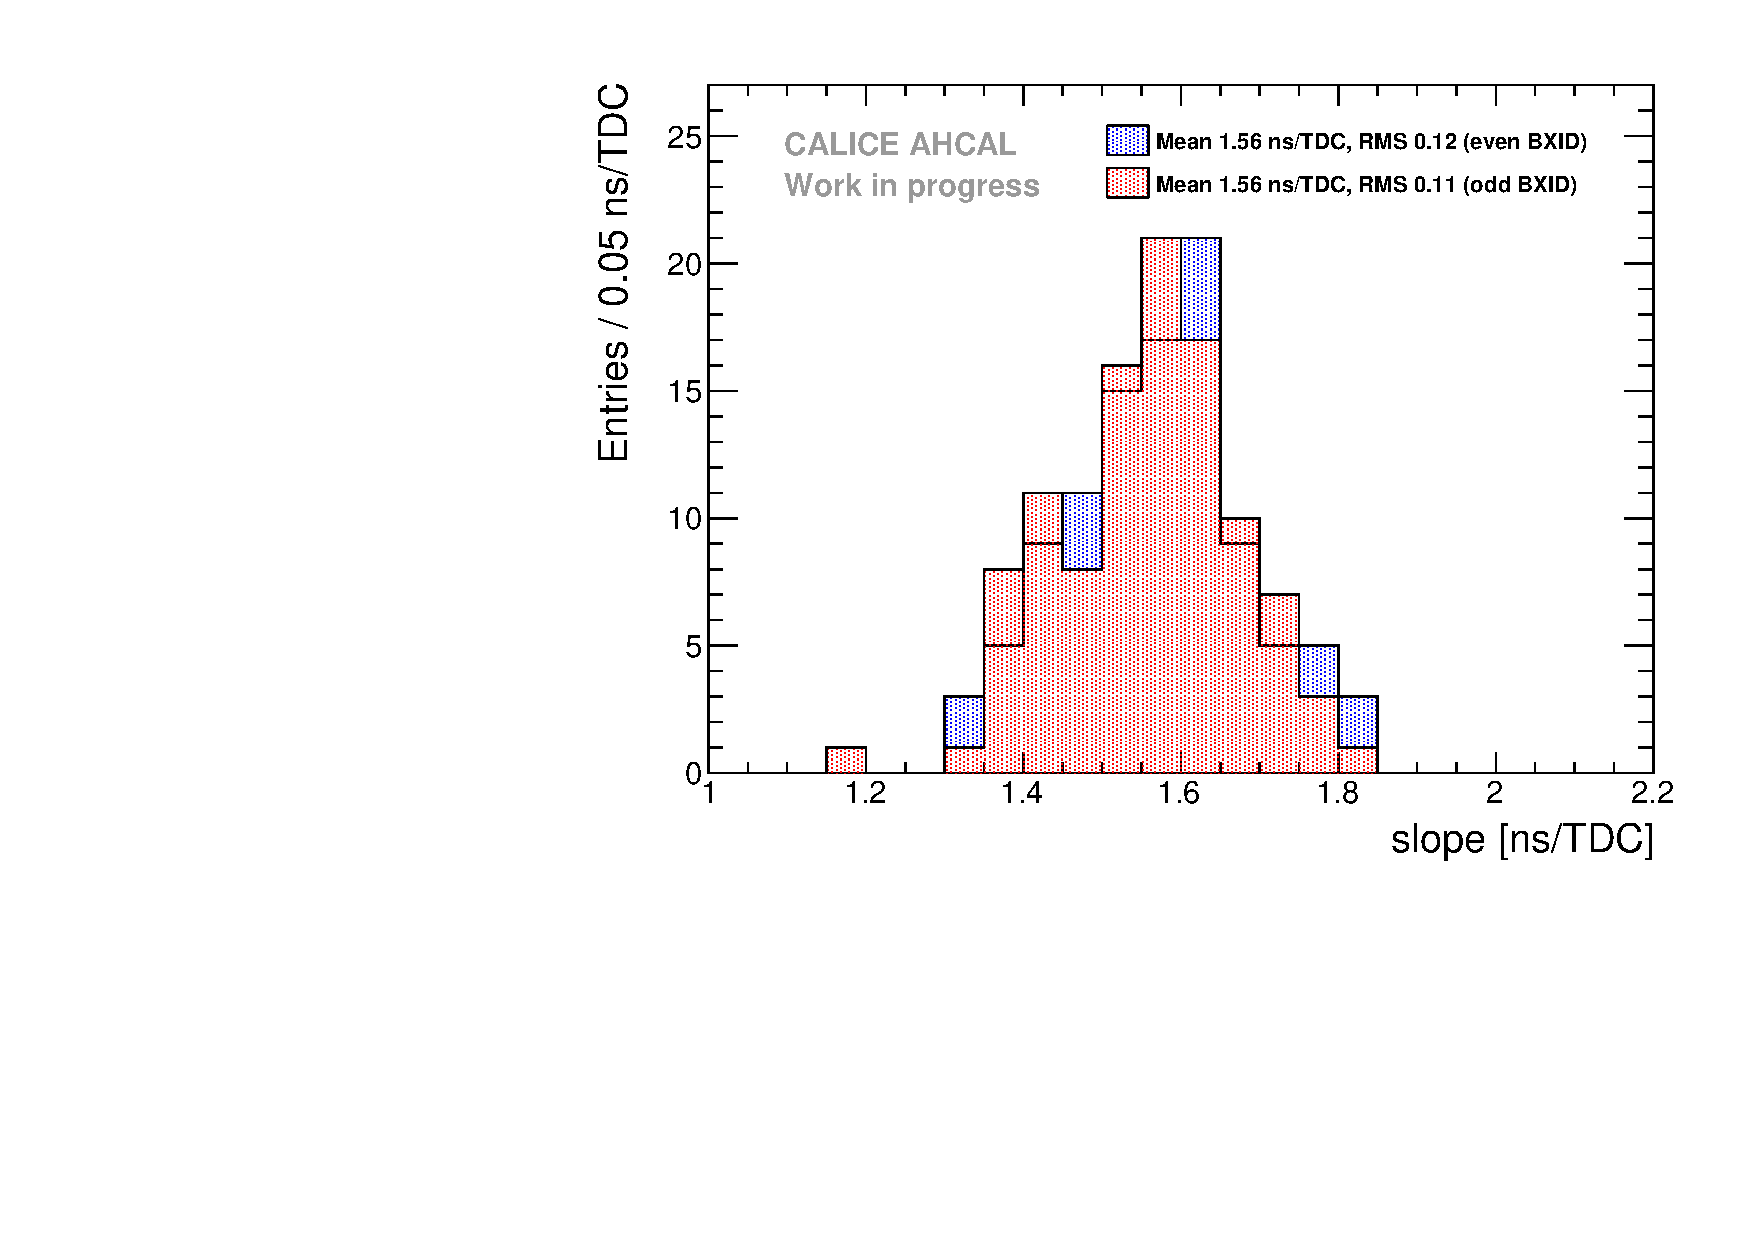
\includegraphics[width=0.7\linewidth]{chap5/fig_AHCAL_timing/Muons/SlopesTDC}
	\caption{Distribution of the fitted slopes for even and odd bunch-crossing IDs. $\mu_{odd}$ = 1.564 ns/TDC, RMS$_{odd}$ = 0.121, $\mu_{even}$ = 1.556 ns/TDC, RMS$_{even}$ = 0.113. All the 208 TDC slopes were extracted.} \label{fig:slope_time}
\end{figure}

\subsection{Determination of the time of first hit}

\subsubsection{Time reference}
\label{subsection:time_ref}

To reconstruct the time of the first hit in a channel, the measured time of a hit needs to be compared to the time of a reference trigger. The trigger signals described in subsection \ref{subsec:trigger} are calibrated using the same method as explained above with the addition that all memory cells are extracted for these channels to guaranty the most accurate result.

After time calibration of the hit, events are selected by requiring that T$_{12}$, T$_{13}$ and T$_{14}$ are present in the event in a certain amplitude range to reject noise hits from theses channels. In addition, as these channels receive exactly the same signal from the NIM-logic at the same time, a quadratic correction is applied to ensure that they match in time as shown in figure \ref{fig:Corr_T12T14}. The correction is performed by correcting the time of T$_{12}$ and T$_{13}$ compared to the time of T$_{14}$. The figure \ref{fig:T0_Correction} shows that the correction reduces the spread of the trigger channels w.r.t to each other. The resulting resolution for the reference trigger signal is around 4-5 ns. This resolution from the electronics contributes to the final timing resolution obtained.

\begin{figure}[htbp!]
	\begin{subfigure}[t]{0.5\textwidth}
		\centering
		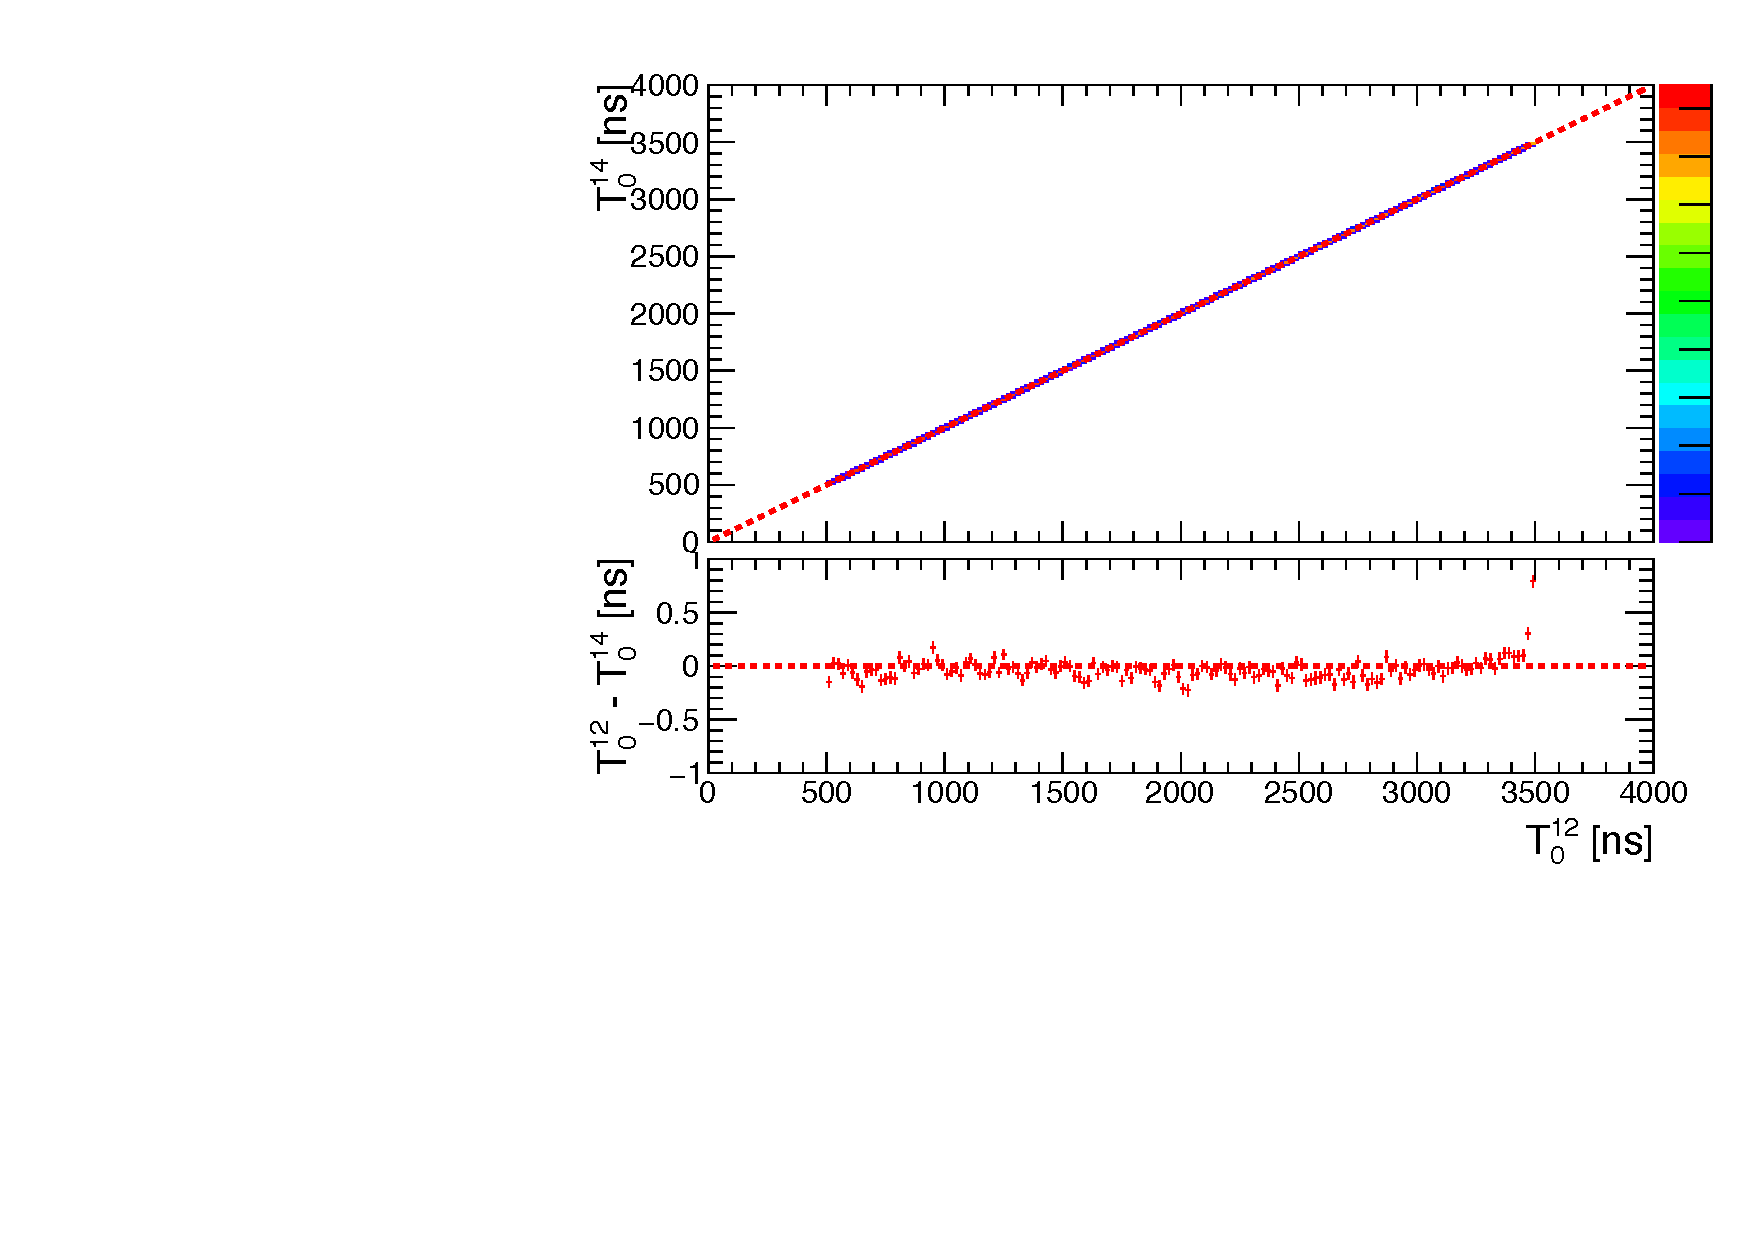
\includegraphics[width=1\textwidth]{chap5/fig_AHCAL_timing/T0s/Correlation_T12vsT14_TDC2ns.pdf}
		\caption{Time correlation the reference triggers T$_{12}$ and T$_{14}$.}\label{fig:Corr_T12T14}
	\end{subfigure}
	\hfill
	\begin{subfigure}[t]{0.5\textwidth}
		\centering
		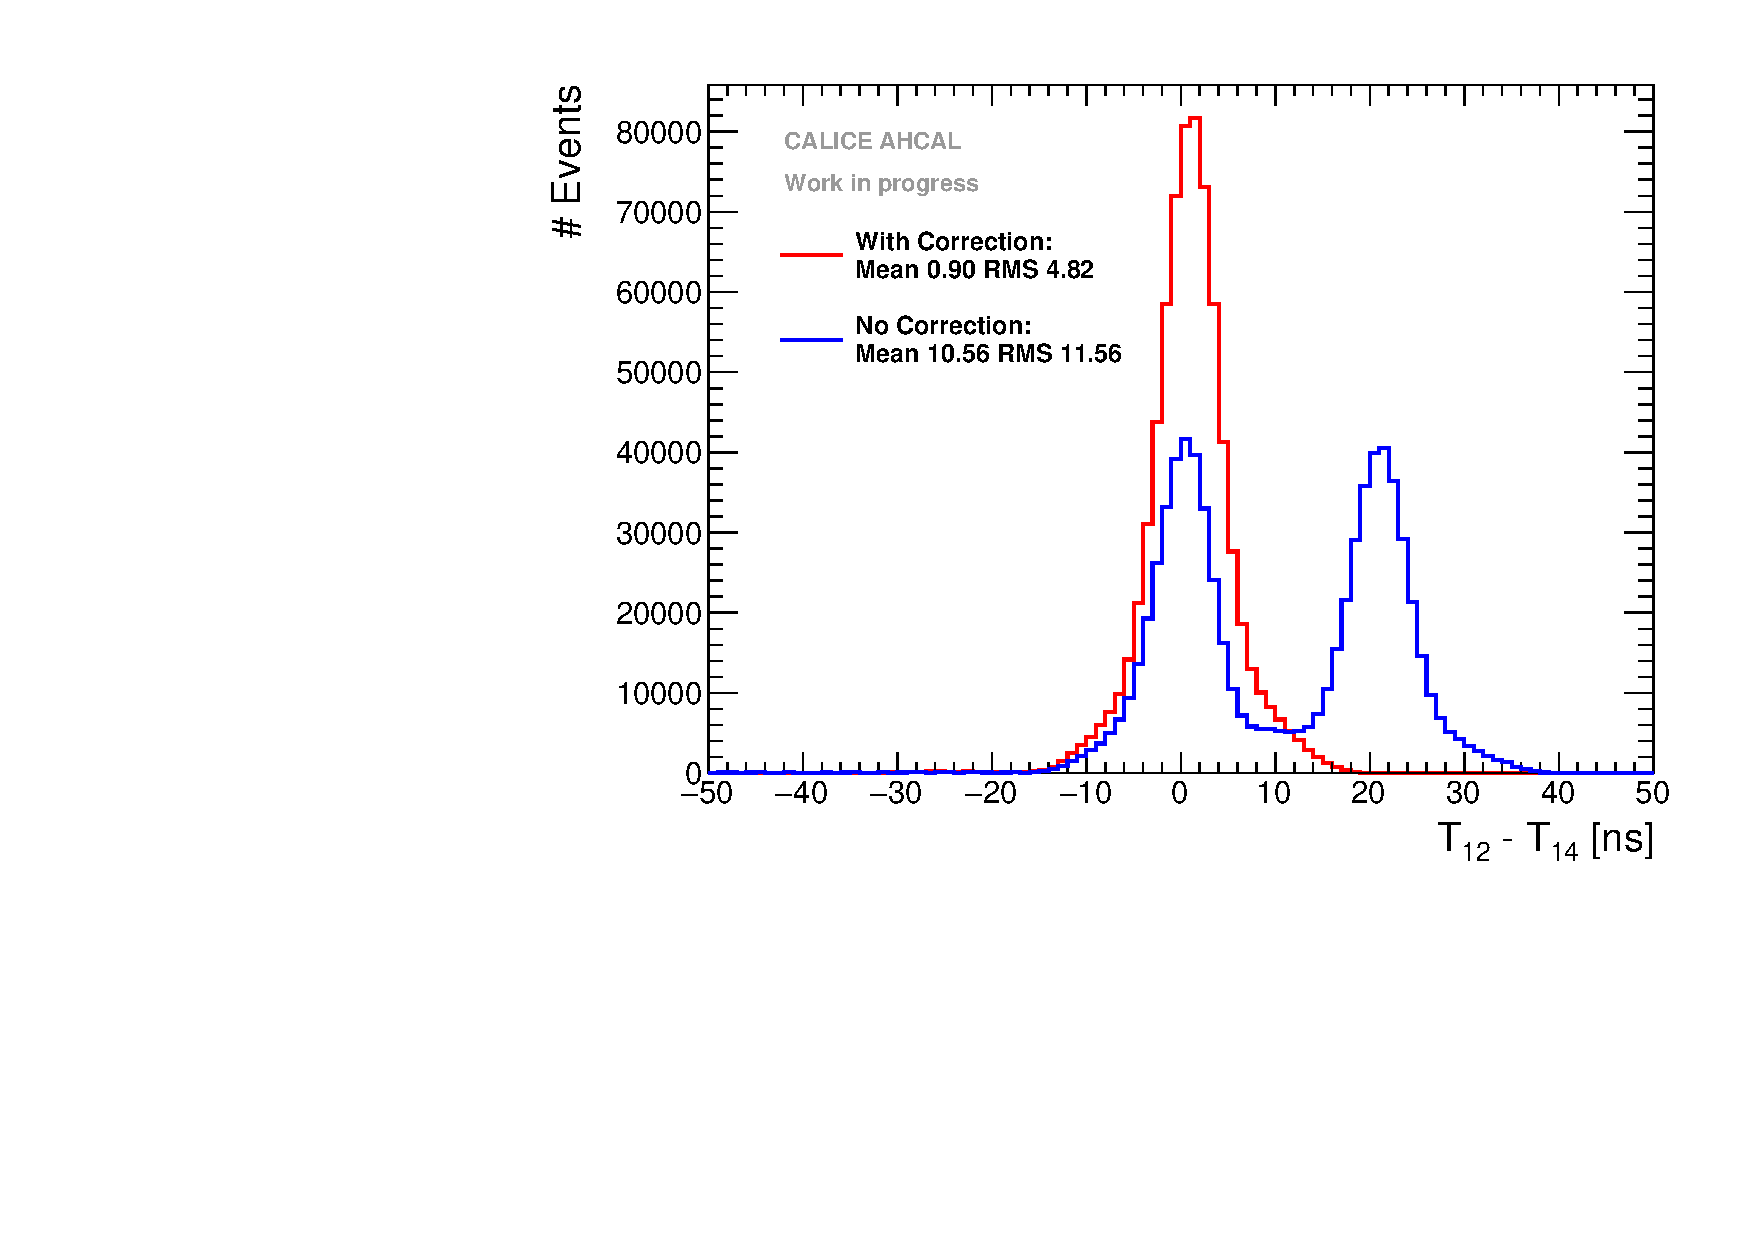
\includegraphics[width=1\textwidth]{chap5/fig_AHCAL_timing/T0s/T0_Resolution_5.pdf}
		\caption{Time difference between the trigger channels before and after correction for T$_{12}$ and T$_{14}$.}	\label{fig:T0_Correction}
	\end{subfigure}
	\caption{\subref{fig:Corr_T12T14}) The top plot shows the time correlation between the references T$_{12}$ and T$_{14}$. The bottom plot show the profile of the difference between them. \subref{fig:T0_Correction}) The histogram in blue shows the difference between the channels before correction, the histogram in red shows the difference after correction. $\mu$ = 10.6 ns, RMS = 11.6 ns, $\mu_{corrected}$ = 0.9 ns, RMS$_{corrected}$ = 4.8 ns. The two visible peaks in blue are due to pedestal values being different dependant of the bunch-crossing.}
\end{figure}

In a next step, to reduce the uncertainty made on the time of the trigger, the time reference $T_{ref}$ is calculated using the mean of T$_{12}$, T$_{13}$ and T$_{14}$ and its associated error $\sigma_{ref}$ as shown in eq. \ref{eq:tref} \& \ref{eq:tref_err}. A cut of 4 ns is performed on $\sigma_{ref}$ to reject events with a too large error on the time of the trigger reference. Finally only hits with a TDC value between 500 and 3500 were considered to avoid TDC ramp edge effects.

\begin{equation} \label{eq:tref}
	\text{T}_{ref} = \frac{\text{T}_{12} + \text{T}_{13} + \text{T}_{14}}{3}
\end{equation}
\begin{equation} \label{eq:tref_err}
	\sigma_{ref}^2 = \frac{ (\text{T}_{12} - \text{T}_{ref})^2 + (\text{T}_{13} - \text{T}_{ref})^2  + (\text{T}_{14} - \text{T}_{ref})^2 }{6}
\end{equation}

Since the absolute time between the passage of a muon and the trigger of a channel is not known due to cabling and the trigger electronics, the time offset relative to the trigger is determined from data. Muons are quasi-instantaneous particles thus the time of the first hit distribution for each channel, memory cells and BXID has to be shifted to \textit{t=0}. This shifting procedure takes into account the delay time of the trigger due to cabling and the NIM-logic as well as possible mis-calibrations in pedestals. Only memory-cells containing more than 100 events are considered.

This offset is determined by iteration requiring at least 4 prompt hits i.e hits in the range from -20 to 20 ns of the event. This is required to remove noisy channels and ensure a good calibration of the offset. In this way, 18338 individual offsets are extracted from data. A distribution of the extracted offsets using muon data can be seen in figure \ref{fig:offset_trigger_distribution}. The mean value of -150 ns is in the expected order for the cabling and NIM-logic delay. The figure \ref{fig:BXID_offset} shows that individual offsets have to be extracted for each BXID and indicates that a pedestal value per BXID should be needed.

\begin{figure}[htbp!]
	\begin{subfigure}[t]{0.5\textwidth}
		\centering
		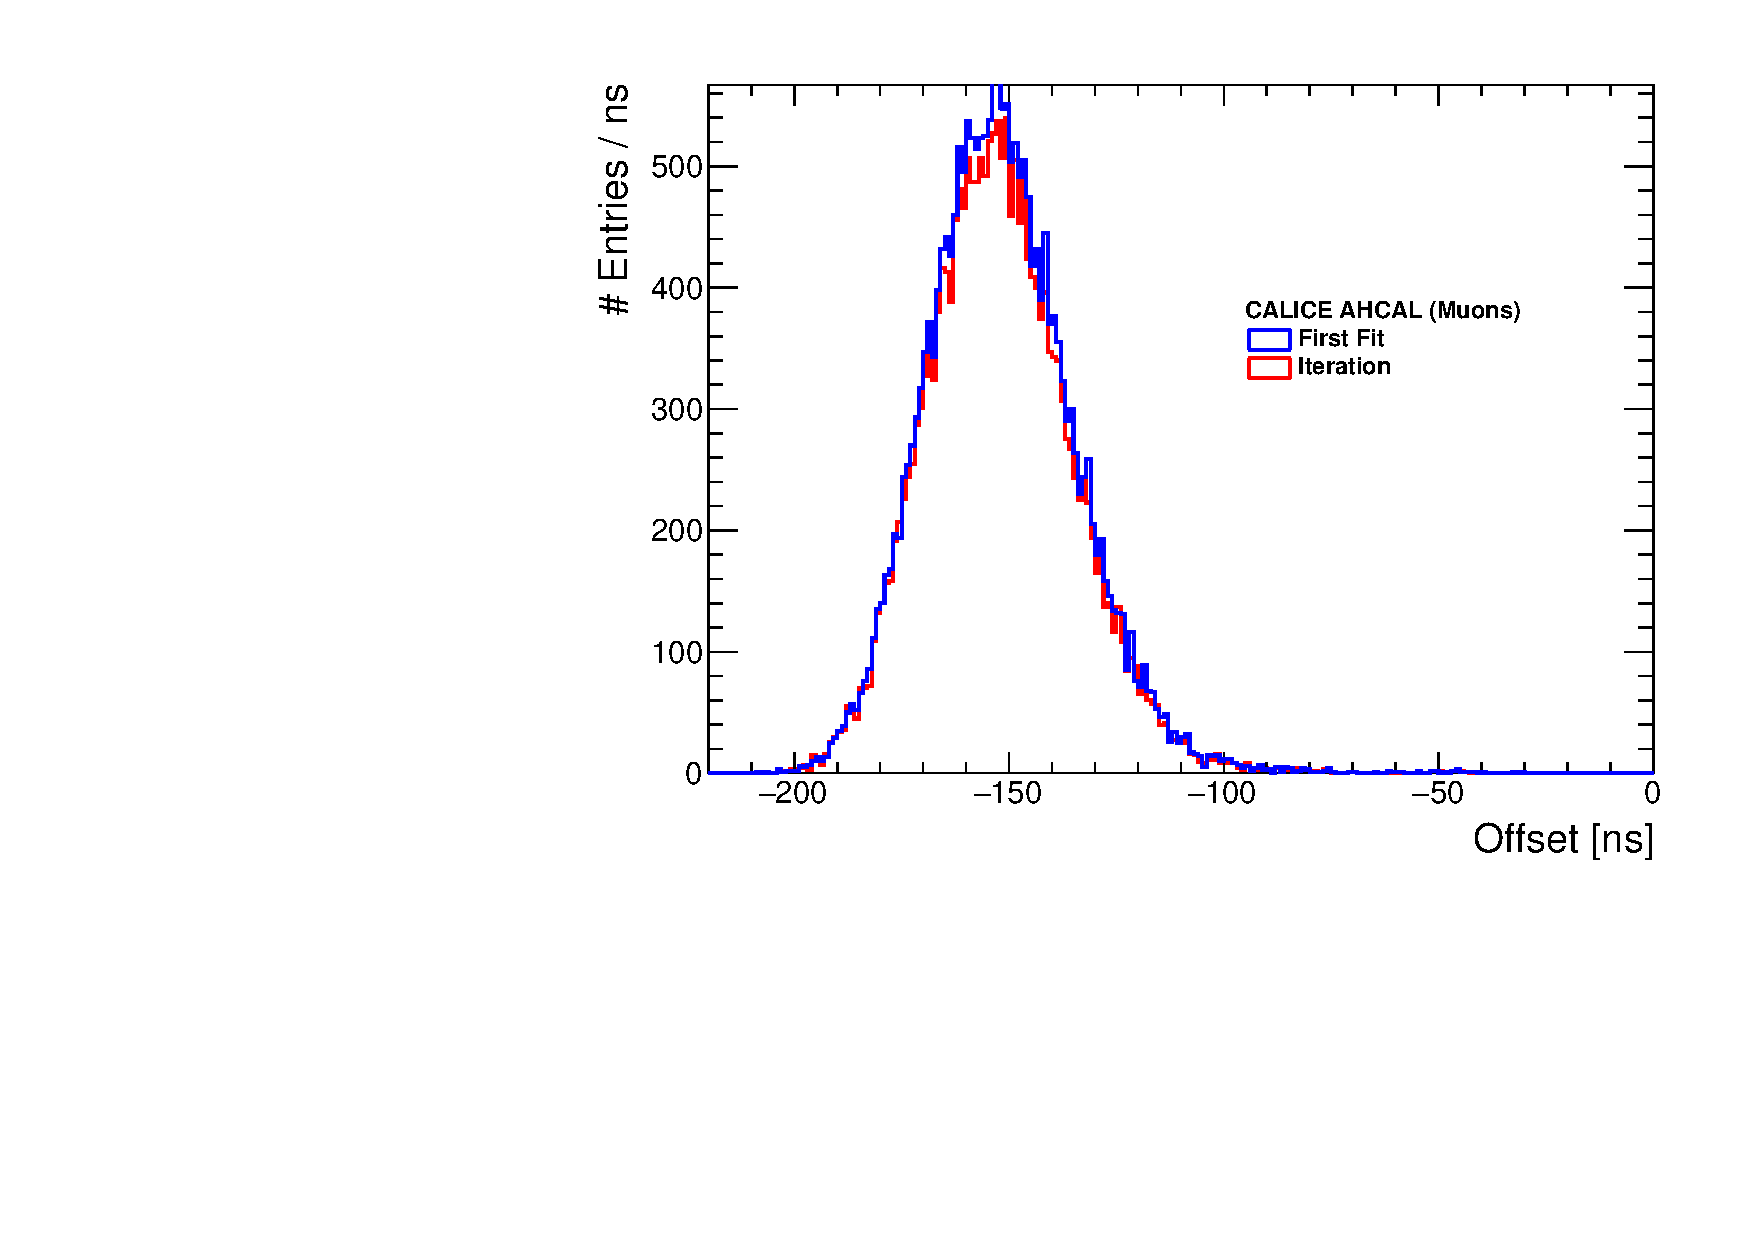
\includegraphics[width=1\textwidth]{chap5/fig_AHCAL_timing/Muons/ExtractedOffsets.pdf}
		\caption{Distribution of the offset used to correct for the trigger delay.}\label{fig:offset_trigger_distribution}
	\end{subfigure}
	\hfill
	\begin{subfigure}[t]{0.5\textwidth}
		\centering
		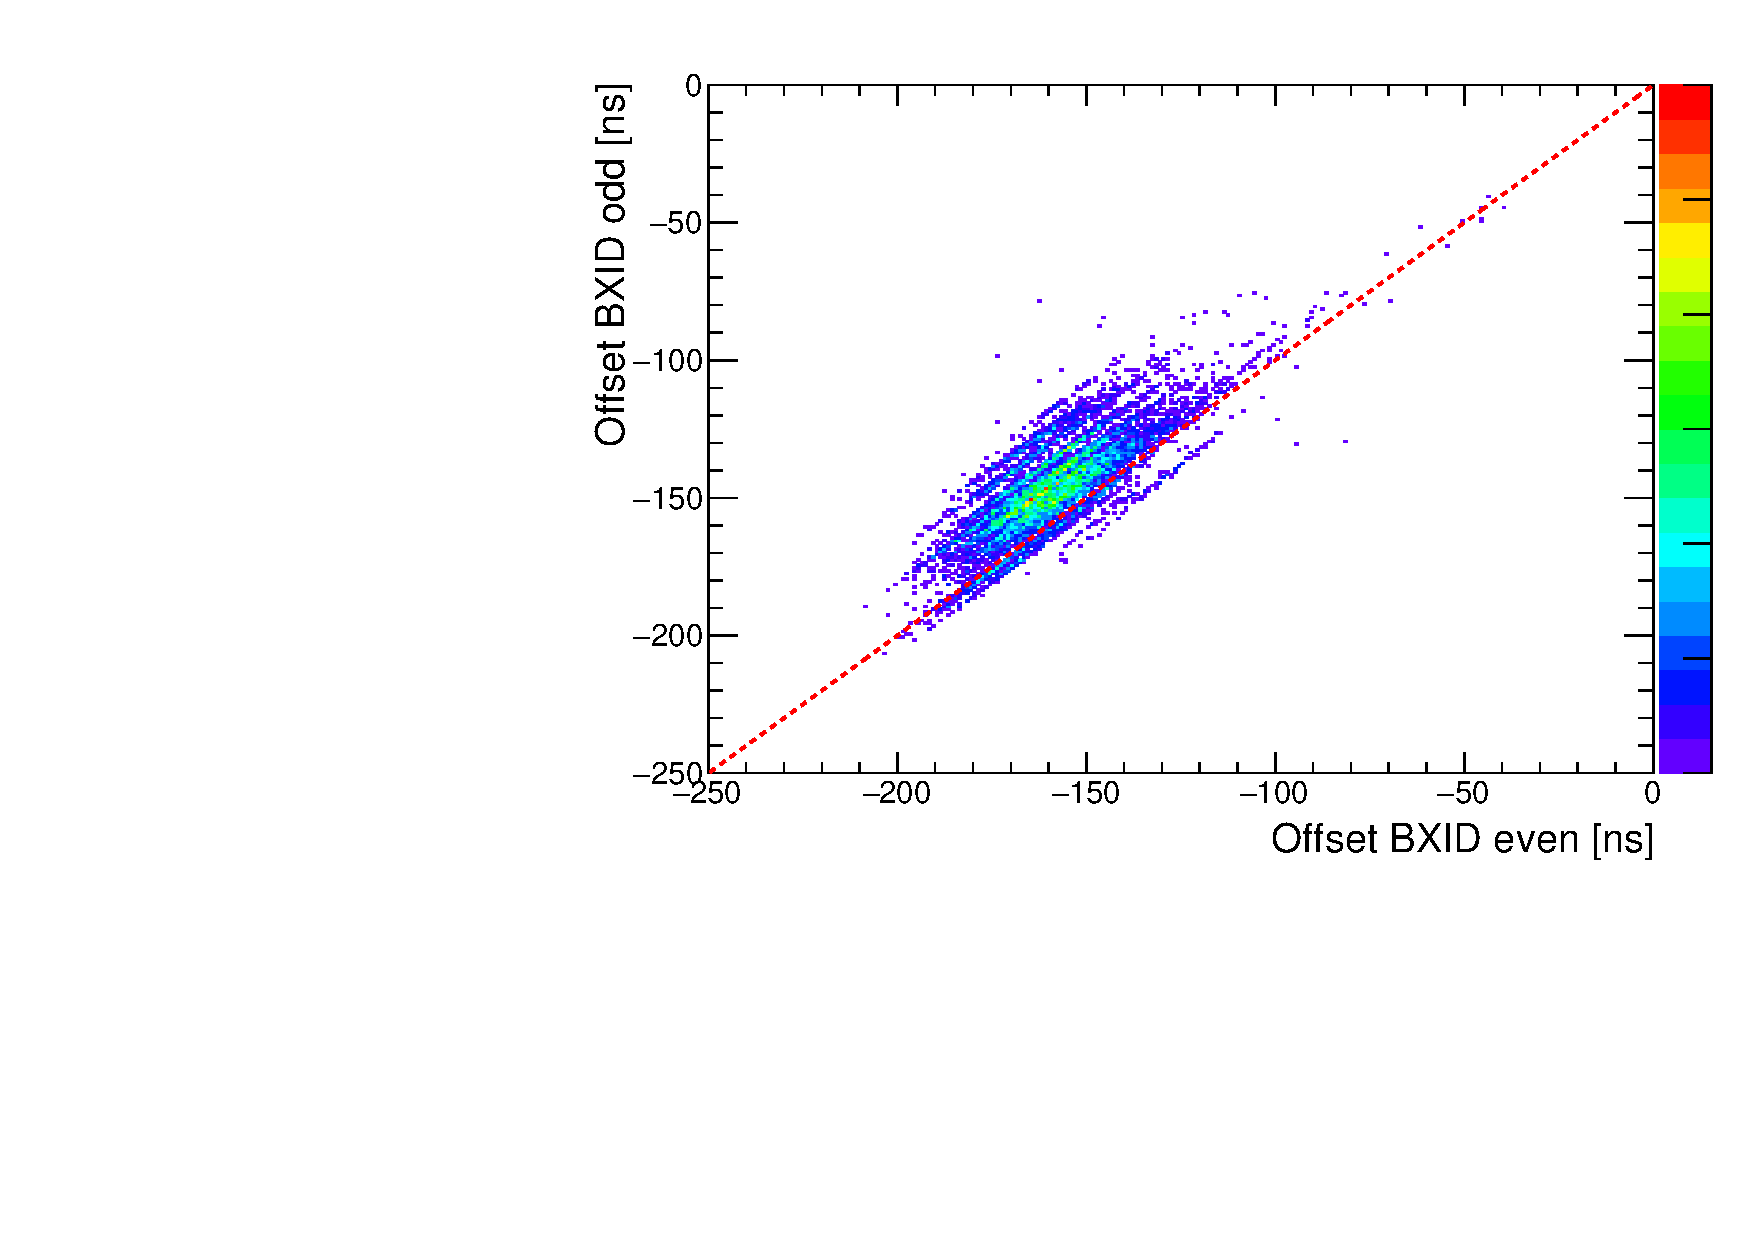
\includegraphics[width=1\textwidth]{chap5/fig_AHCAL_timing/Muons/CorrelationOffsets_BXID.pdf}
		\caption{Correlation between offsets extracted for even and odd BXID.}\label{fig:BXID_offset}
	\end{subfigure}
	\caption{\subref{fig:offset_trigger_distribution}) Extracted offset used to correct for the trigger delay signal. The mean delay of the trigger is $\sim$ 150 ns and is in the expected order. \subref{fig:BXID_offset}) Correlation between offsets extracted for BXID even and odd. The shift of the correlation indicates that the correction is BXID-dependant certainly due to difference in pedestal values for even/add BXIDs.}
\end{figure}

\subsubsection{Time of the first hit distribution}

After the selection and calibration, the time of the first hit (T$_{fH}$) can be obtained by plotting the distribution of T$_{chn}$ - T$_{ref}$ as shown in figure \ref{fig:timing_nocorrection}. The time resolution (RMS) shown in figure \ref{fig:timing_nocorrection} obtained by combining all layers excluding layer 11 is around 5.65 ns by just applying the time calibration on the data. This is far from the desired time resolution of 1 ns and is dominated by the resolution of the time reference. Some improvements are still possible as described in the following. An asymmetry can be seen in the time distribution to the left. It is likely coming from the non-linearity of the TDC ramp as explained in the next subsection.

Each layer was also looked at individually as shown in figure \ref{fig:reso_nocorrection}. A comparison between a gaussian fit and the RMS of the distribution is done. All layers are very similar in terms of time resolution and gaussian-like. The layer 6 and 10 present a higher time resolution which was expected due to the bad quality of these layers. The discrepancy observed for the layer 11 is most likely due to an electronic problem in the TDC voltage ramp of all the chips on that layer.

\begin{figure}[htbp!]
	\begin{subfigure}[t]{0.5\textwidth}
		\centering
		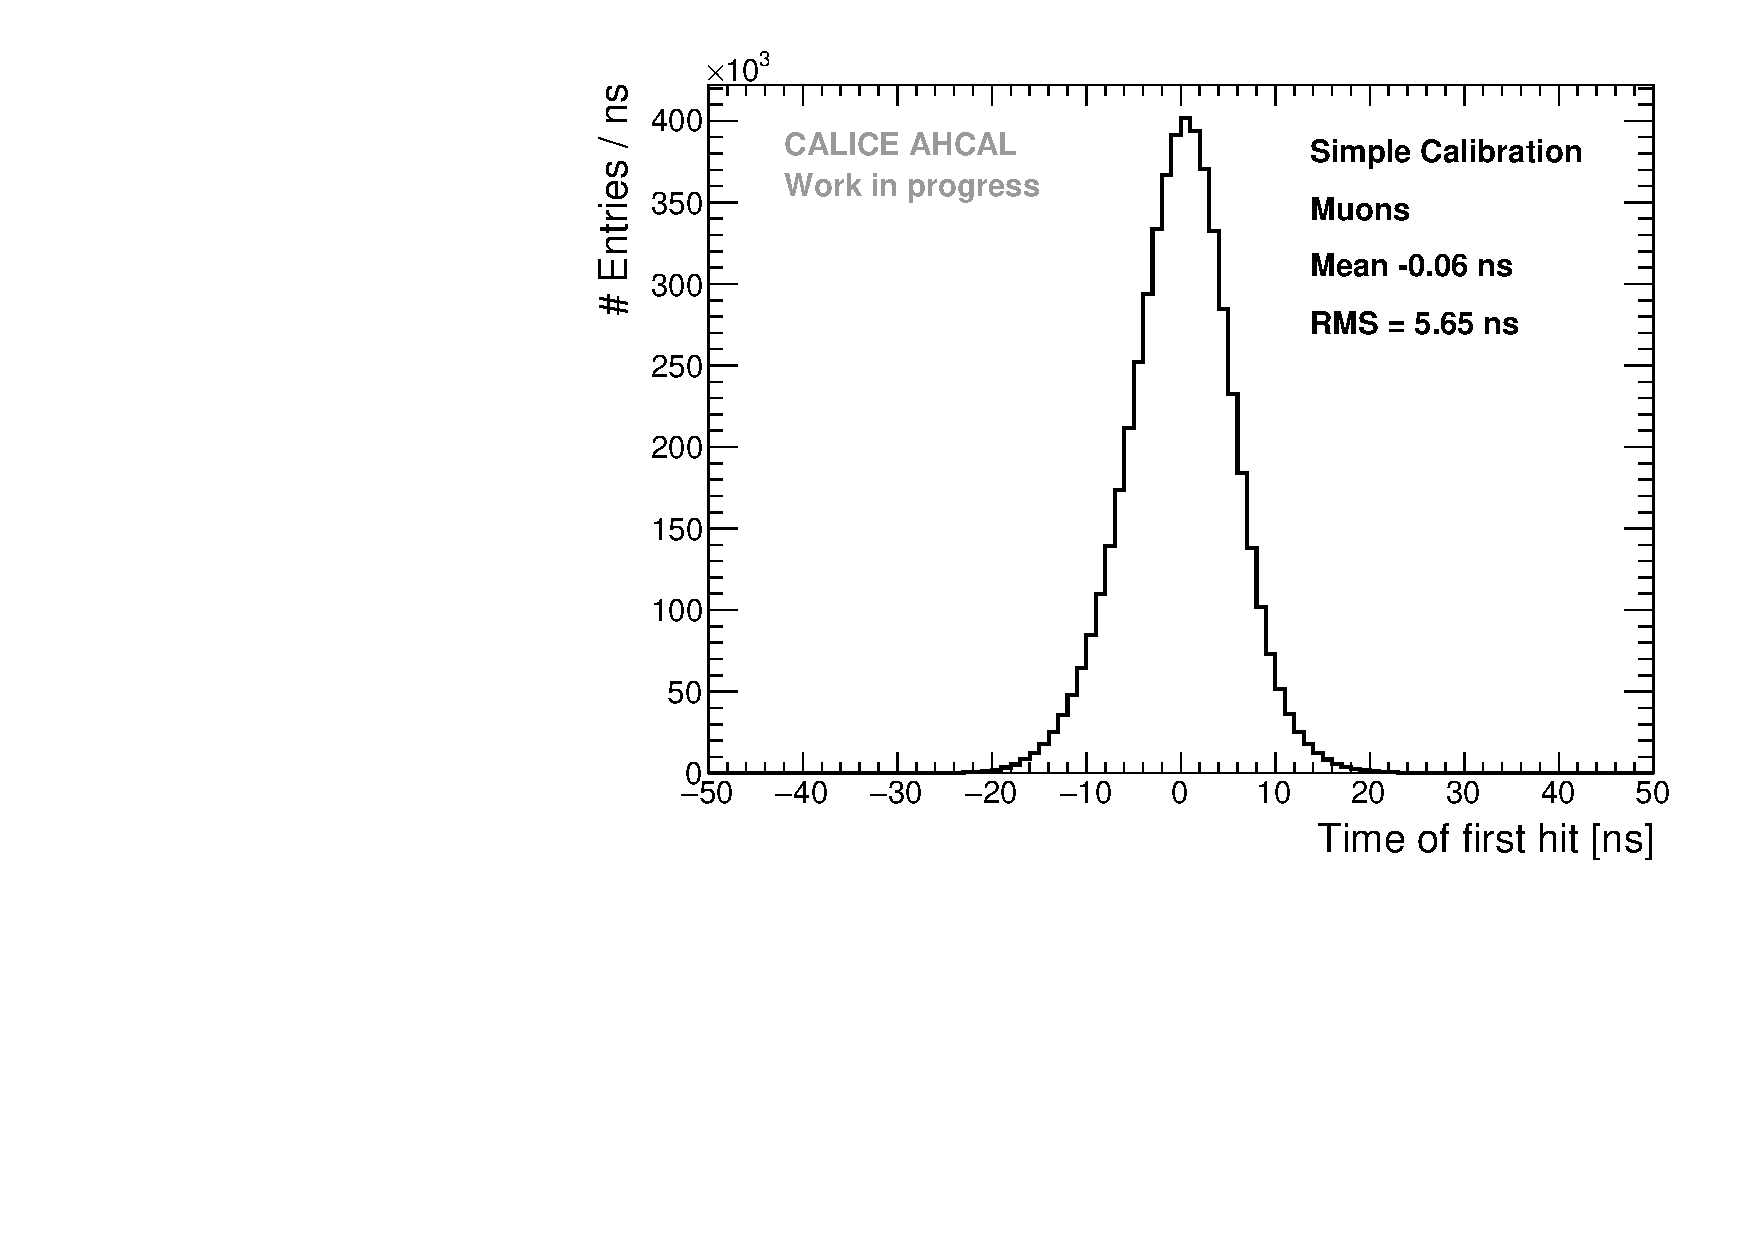
\includegraphics[width=1\textwidth]{chap5/fig_AHCAL_timing/Muons/Timing_AHCAL_noCorrections.pdf}
		\caption{Timing for all layers in the AHCAL excluding layer 11.}\label{fig:timing_nocorrection}
	\end{subfigure}
	\hfill
	\begin{subfigure}[t]{0.5\textwidth}
		\centering
		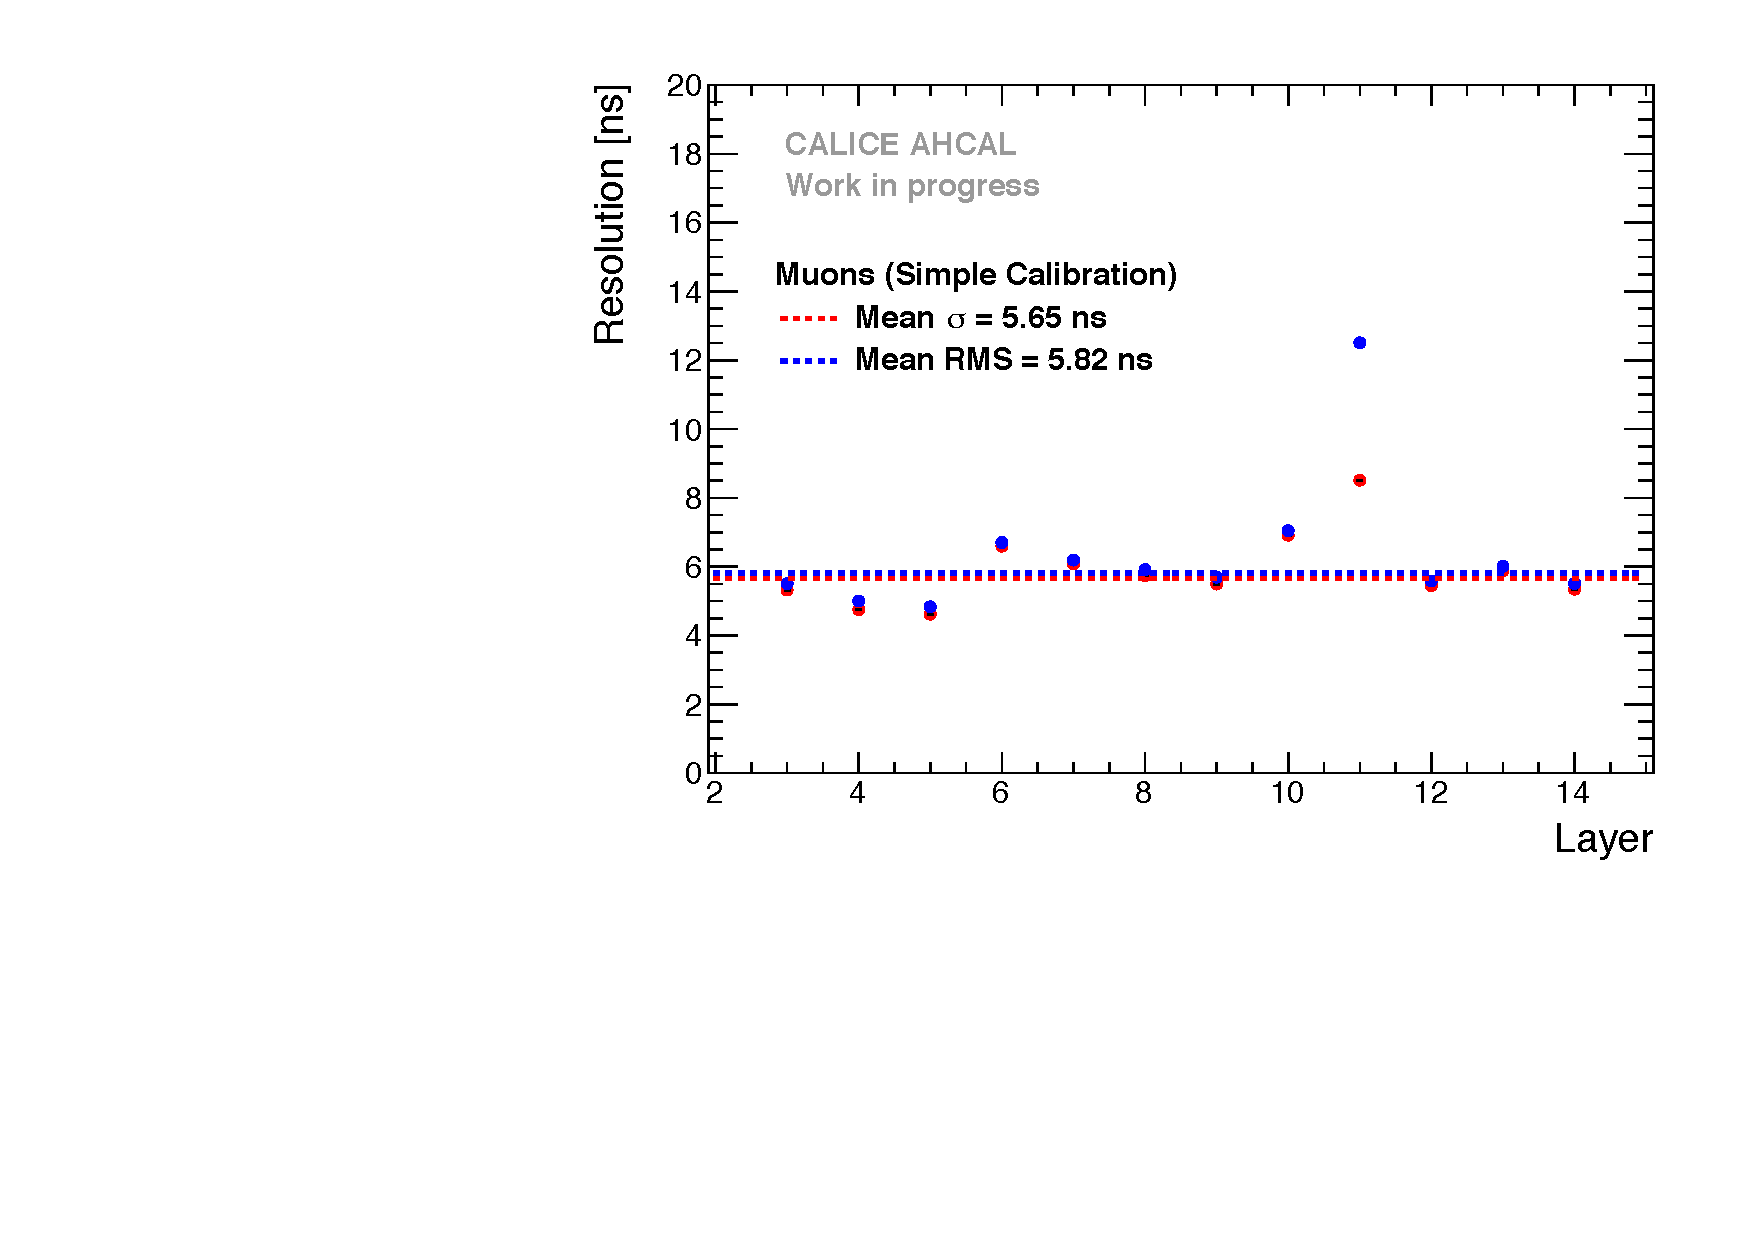
\includegraphics[width=1\textwidth]{chap5/fig_AHCAL_timing/Muons/ResolutionPerModule_noCorrections.pdf}
		\caption{Extracted resolution for all layers in the AHCAL.}\label{fig:reso_nocorrection}
	\end{subfigure}
	\caption{\subref{fig:timing_nocorrection}) Time of the first hit distribution of the AHCAL after the first part of the calibration. $\mu$ = -0.06 ns , RMS = 5.65 ns. The distribution is clearly asymmetric to the left. \subref{fig:reso_nocorrection}) Time resolution for all layers in the AHCAL. The mean RMS time resolution is represented by the blue line.}
\end{figure}

\subsection{Corrections applied to data}

\subsubsection{Ramp non-linearity correction}
\label{subsec:lin_corr}

The calibration relies on the linearity of the TDC voltage ramp in the \textit{SPIROC2B} by measuring the minimum and maximum of the ramp and interpolating the slope assuming a linear ramp. This assumption is not entirely reliable as described in \cite{Hartbrich2011, Brianne2012}. The voltage slope presents a slight kink around the middle leading to a non-linear ramp. For this, a correction of the non-linearity has to be applied.

\begin{figure}[htbp!]
	\begin{subfigure}[t]{0.5\textwidth}
		\centering
		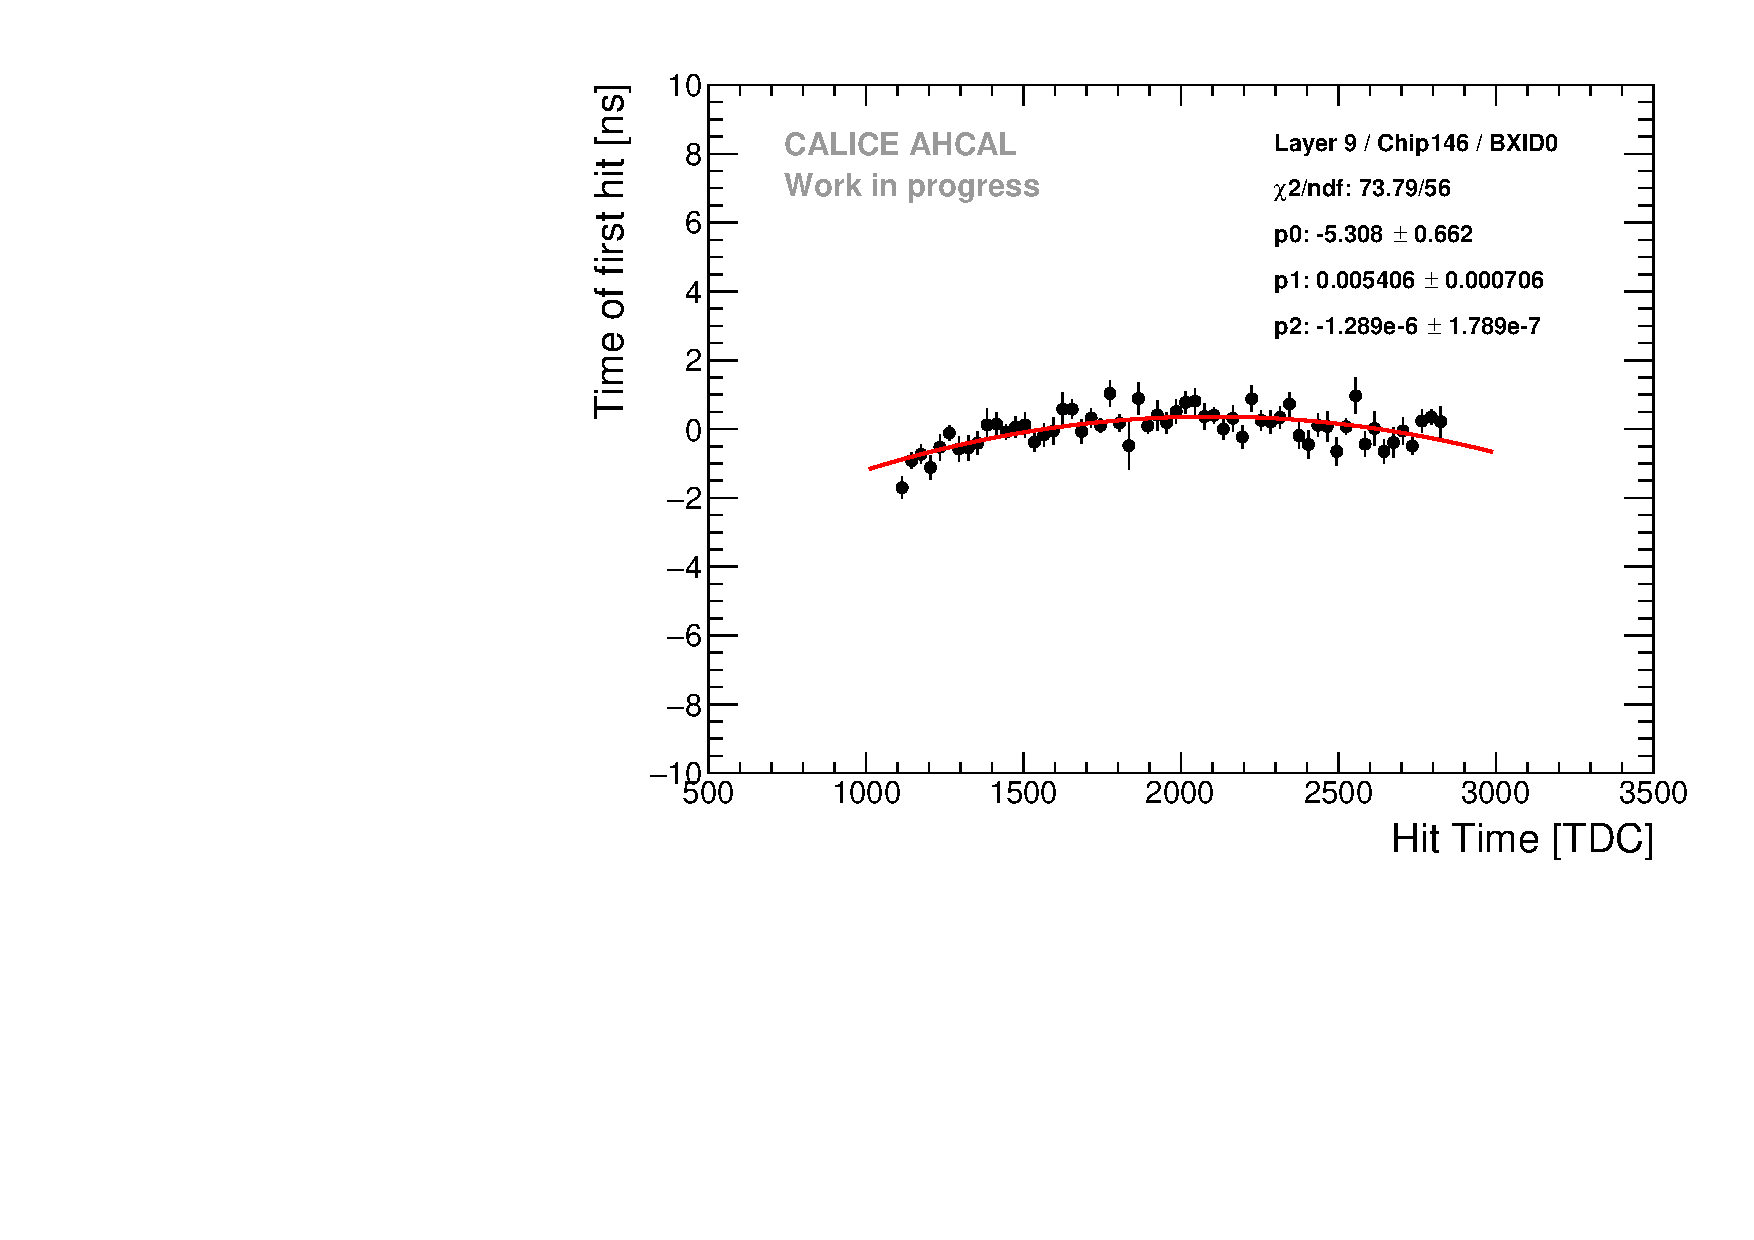
\includegraphics[width=1\textwidth]{chap5/fig_AHCAL_timing/Muons/LinearityCorrection_Module09_Chip146_BXID0.pdf}
		\caption{Quadratic fit of chip 146 (BXID even) on layer 09.}\label{fig:LinCorr}
	\end{subfigure}
	\hfill
	\begin{subfigure}[t]{0.5\textwidth}
		\centering
		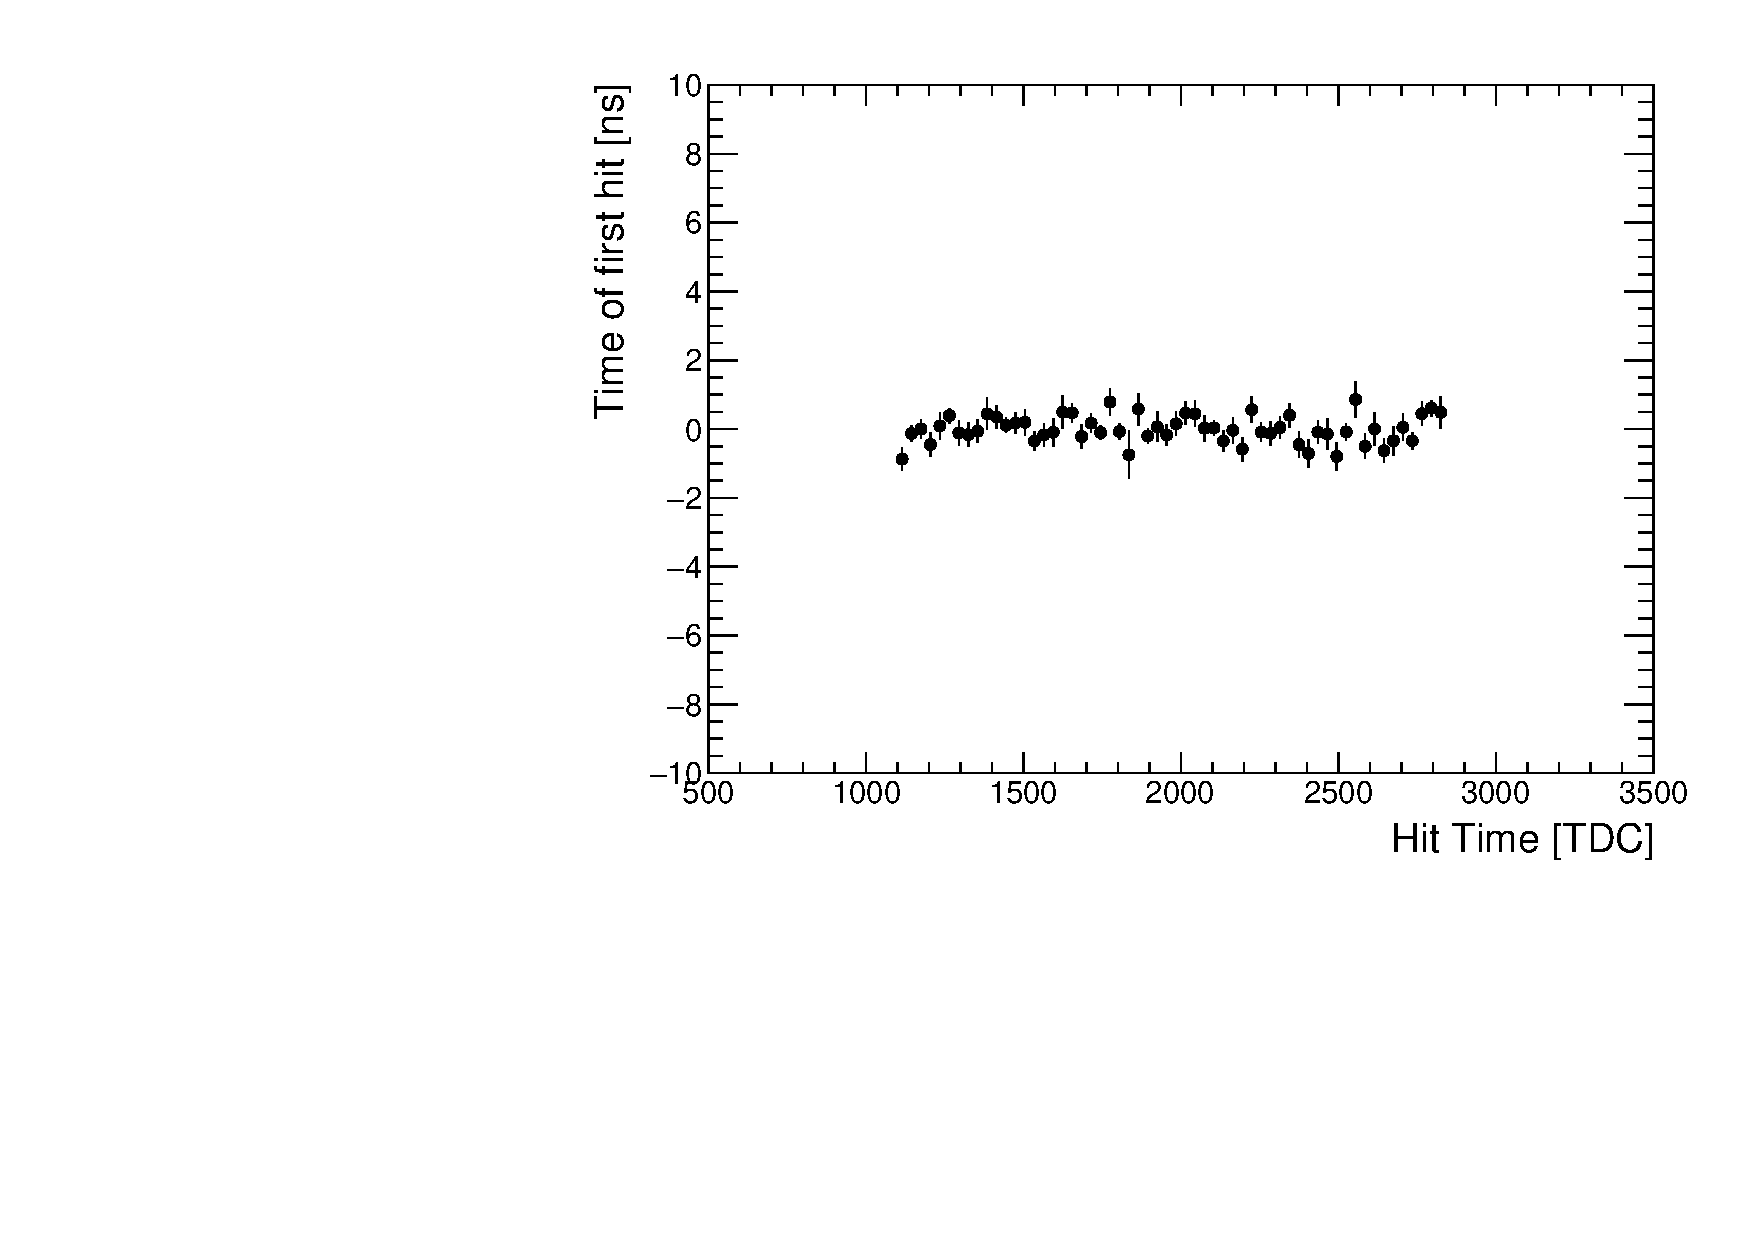
\includegraphics[width=1\textwidth]{chap5/fig_AHCAL_timing/Muons/LinearityCorrection_Module09_Chip146_BXID0_Corrected.pdf}
		\caption{Profile for chip 146 on layer 09 after the non-linearity correction of the ramp.}\label{fig:LinCorr_2}
	\end{subfigure}
	\caption{\subref{fig:LinCorr}) Typical profile of the time of the hit versus the TDC of the hit before the correction. The graph is slightly curved showing that this chip presents a non-linear TDC ramp. The $\chi^2$ of the fit is 1.29. \subref{fig:LinCorr_2}) The correction parameter are applied then on the data to cross-check the quality of the correction. One can see that the curve flattens with the correction applied.}
\end{figure}

By simply looking at the time of the first hit (T$_{fH}$) for each chip and BXID versus the TDC value of the hit, the shape of the graph would indicate how reliable is the assumption of a linear ramp. If the ramp would be perfectly linear, one would obtain a flat graph. To correct for the non-linearity of the ramp, a quadratic fit is performed for each chip and BXID as shown in figure \ref{fig:LinCorr}. The correction needed can be in the order of few nanoseconds. The figure \ref{fig:LinCorr_2} shows the time of first hit as a function of the TDC value of the hit after the correction, the graph looks much flatter.

The non-linearity correction results in an improvement on the timing resolution (RMS) of the AHCAL of about 5.1\% (5.36 ns) as shown in figure \ref{fig:timing_lincorrection}. The assymetry of the time distribution remains and is most likely due to the time reference which is non corrected for the non-linearity as no external time reference for these channels is present. Looking at each layer, as shown on figure \ref{fig:reso_lincorrection}, the time resolution went down by the same amount.

\begin{figure}[htbp!]
	\begin{subfigure}[t]{0.5\textwidth}
		\centering
		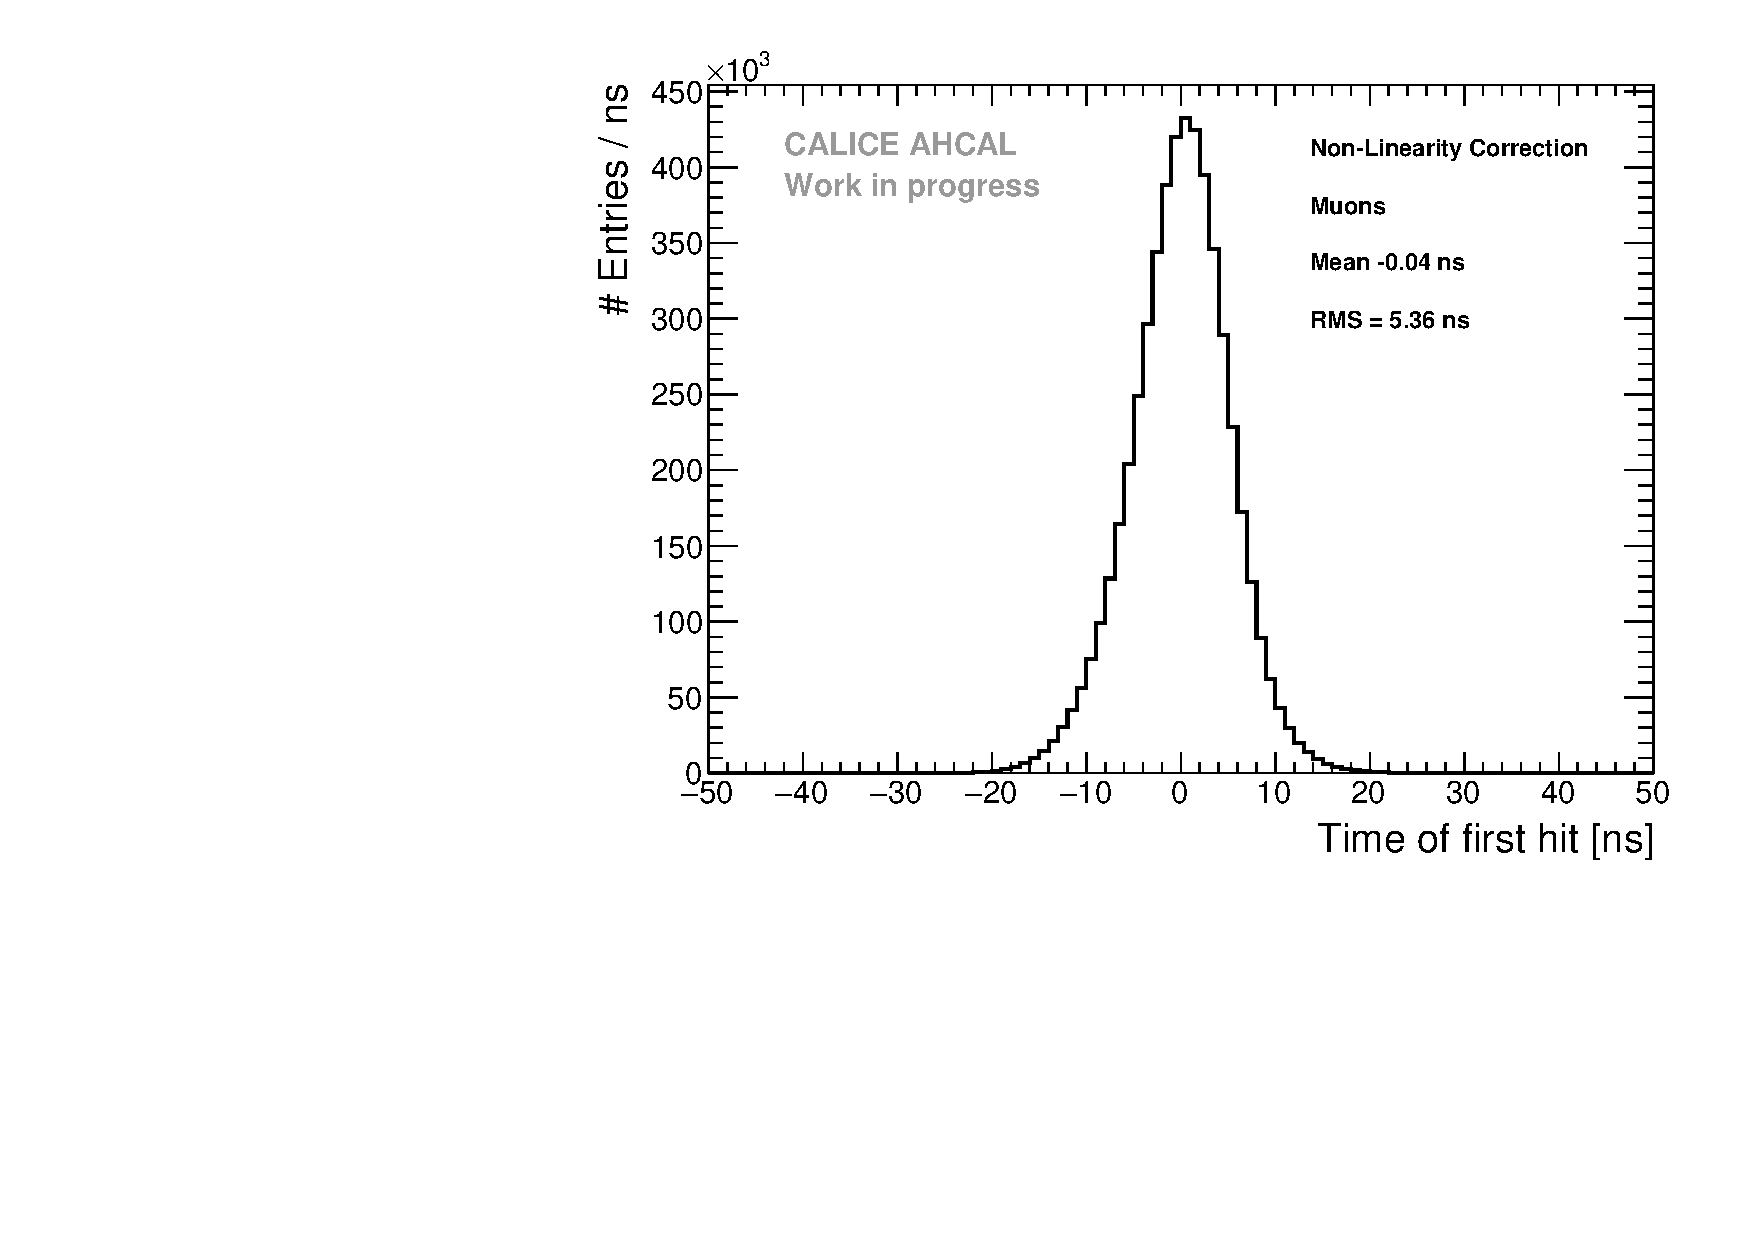
\includegraphics[width=1\textwidth]{chap5/fig_AHCAL_timing/Muons/Timing_AHCAL_LinCorrection.pdf}
		\caption{Timing for all layers in the AHCAL excluding layer 11.}\label{fig:timing_lincorrection}
	\end{subfigure}
	\hfill
	\begin{subfigure}[t]{0.5\textwidth}
		\centering
		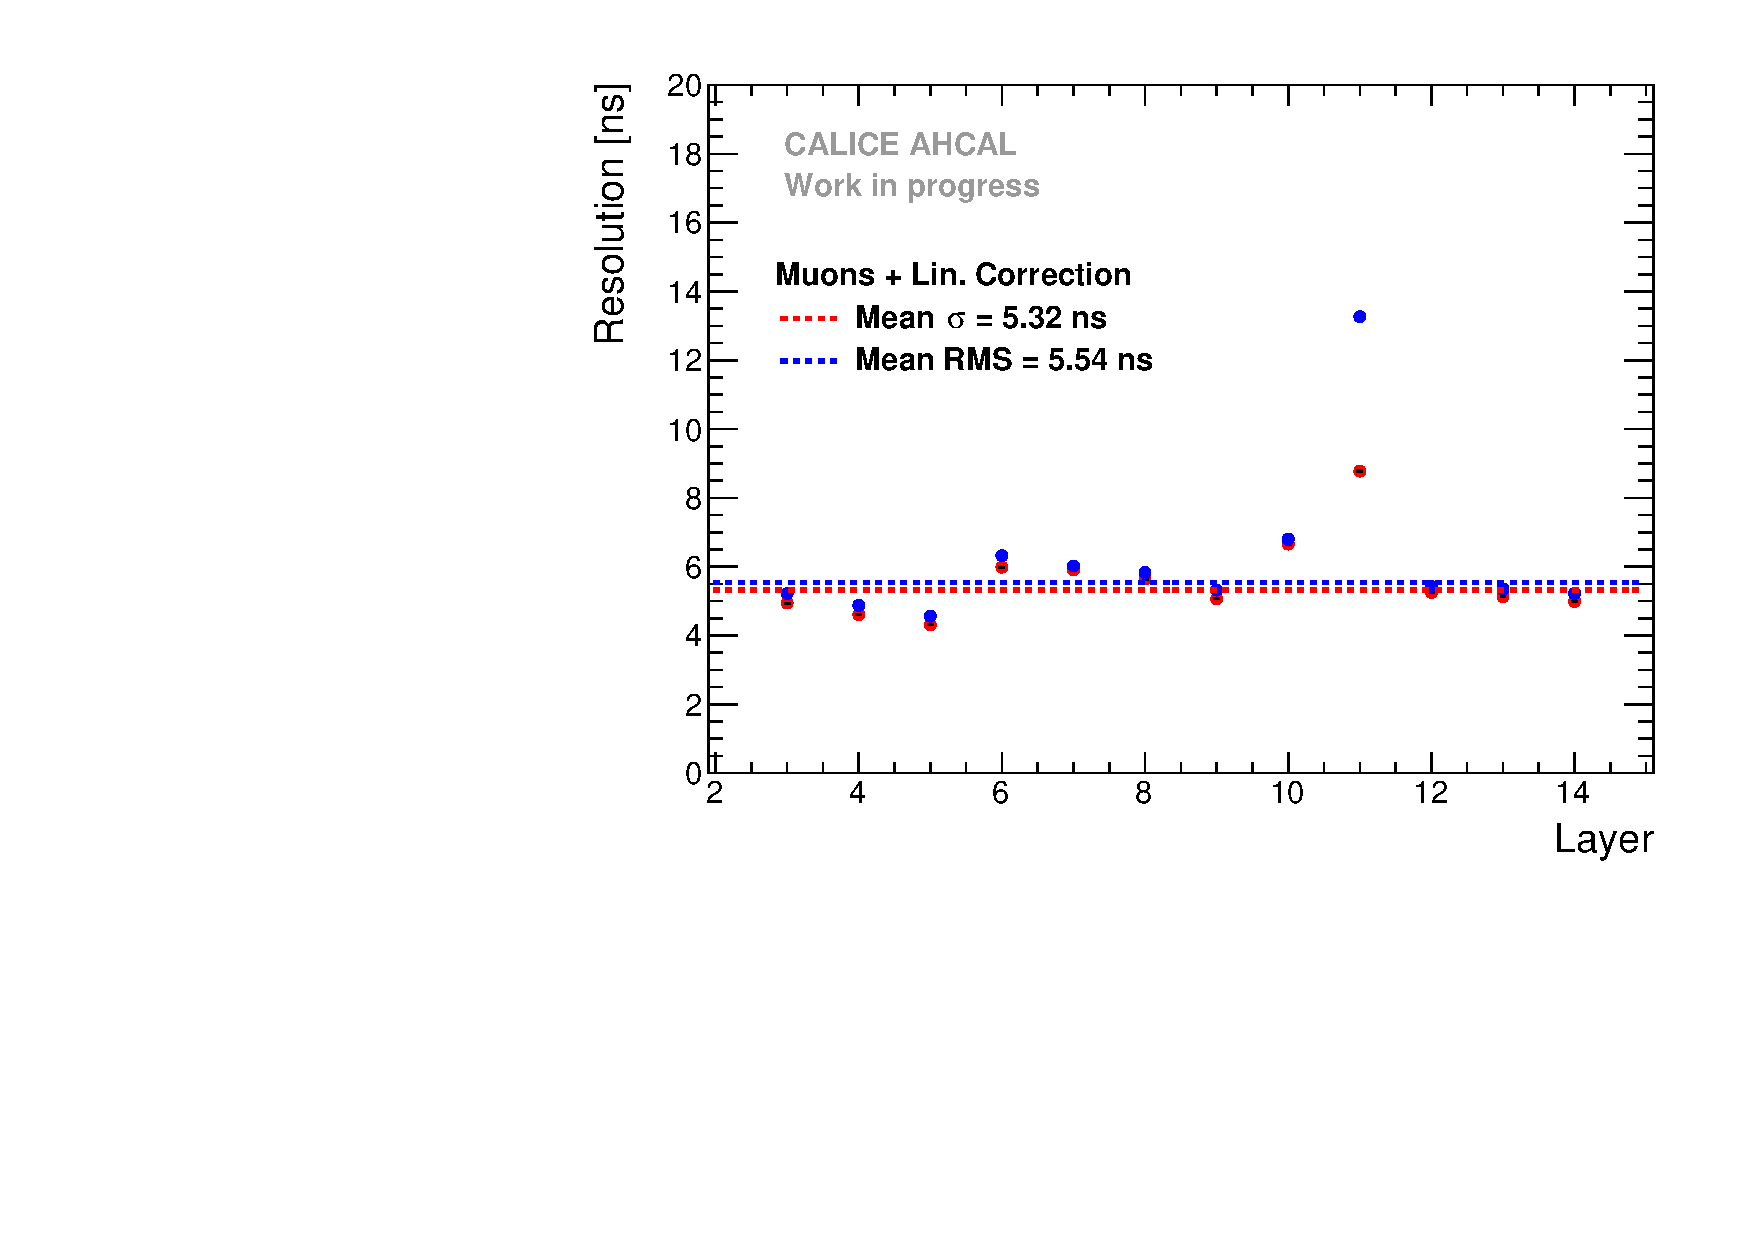
\includegraphics[width=1\textwidth]{chap5/fig_AHCAL_timing/Muons/ResolutionPerModule_LinCorrection.pdf}
		\caption{Extracted resolution for all layers in the AHCAL.}\label{fig:reso_lincorrection}
	\end{subfigure}
	\caption{\subref{fig:timing_lincorrection} Time of the first hit distribution of the AHCAL after the non-linearity correction. $\mu$ = -0.04 ns , RMS = 5.36 ns. \subref{fig:reso_lincorrection} Time resolution for all layers in the AHCAL. The mean RMS is 5.54 ns.}
\end{figure}

\subsubsection{Time Walk correction}
\label{subsec:timewalk}

The time-walk effect is due to the presence of a threshold that induces a time shift between a small amplitude signal and a high amplitude signal. Small amplitude signals will systematically trigger at a later time than high amplitude signals. A correction can be applied on the data by looking at the time of the first hit versus the amplitude of the hit. This might be particularly important for late neutrons signals that generally deposit very little energy in the calorimeter.

The correction is assumed to be the same for all the chips, independent of the position of the threshold of each chip, as hits are cut at 0.5 MIP and most of the chips were having the threshold set-up well below 0.5 MIP. An exponential fit of the form $\text{A} \times e^{-\lambda{}x} + \text{B}$ is performed on the data to extract the parameters needed to correct the time walk effect as shown on figure \ref{fig:time_walk}. The residuals after correction are in the order of few hundreds of picoseconds as seen in figure \ref{fig:time_walk_corr}.

\begin{figure}[htbp!]
	\begin{subfigure}[t]{0.5\textwidth}
		\centering
		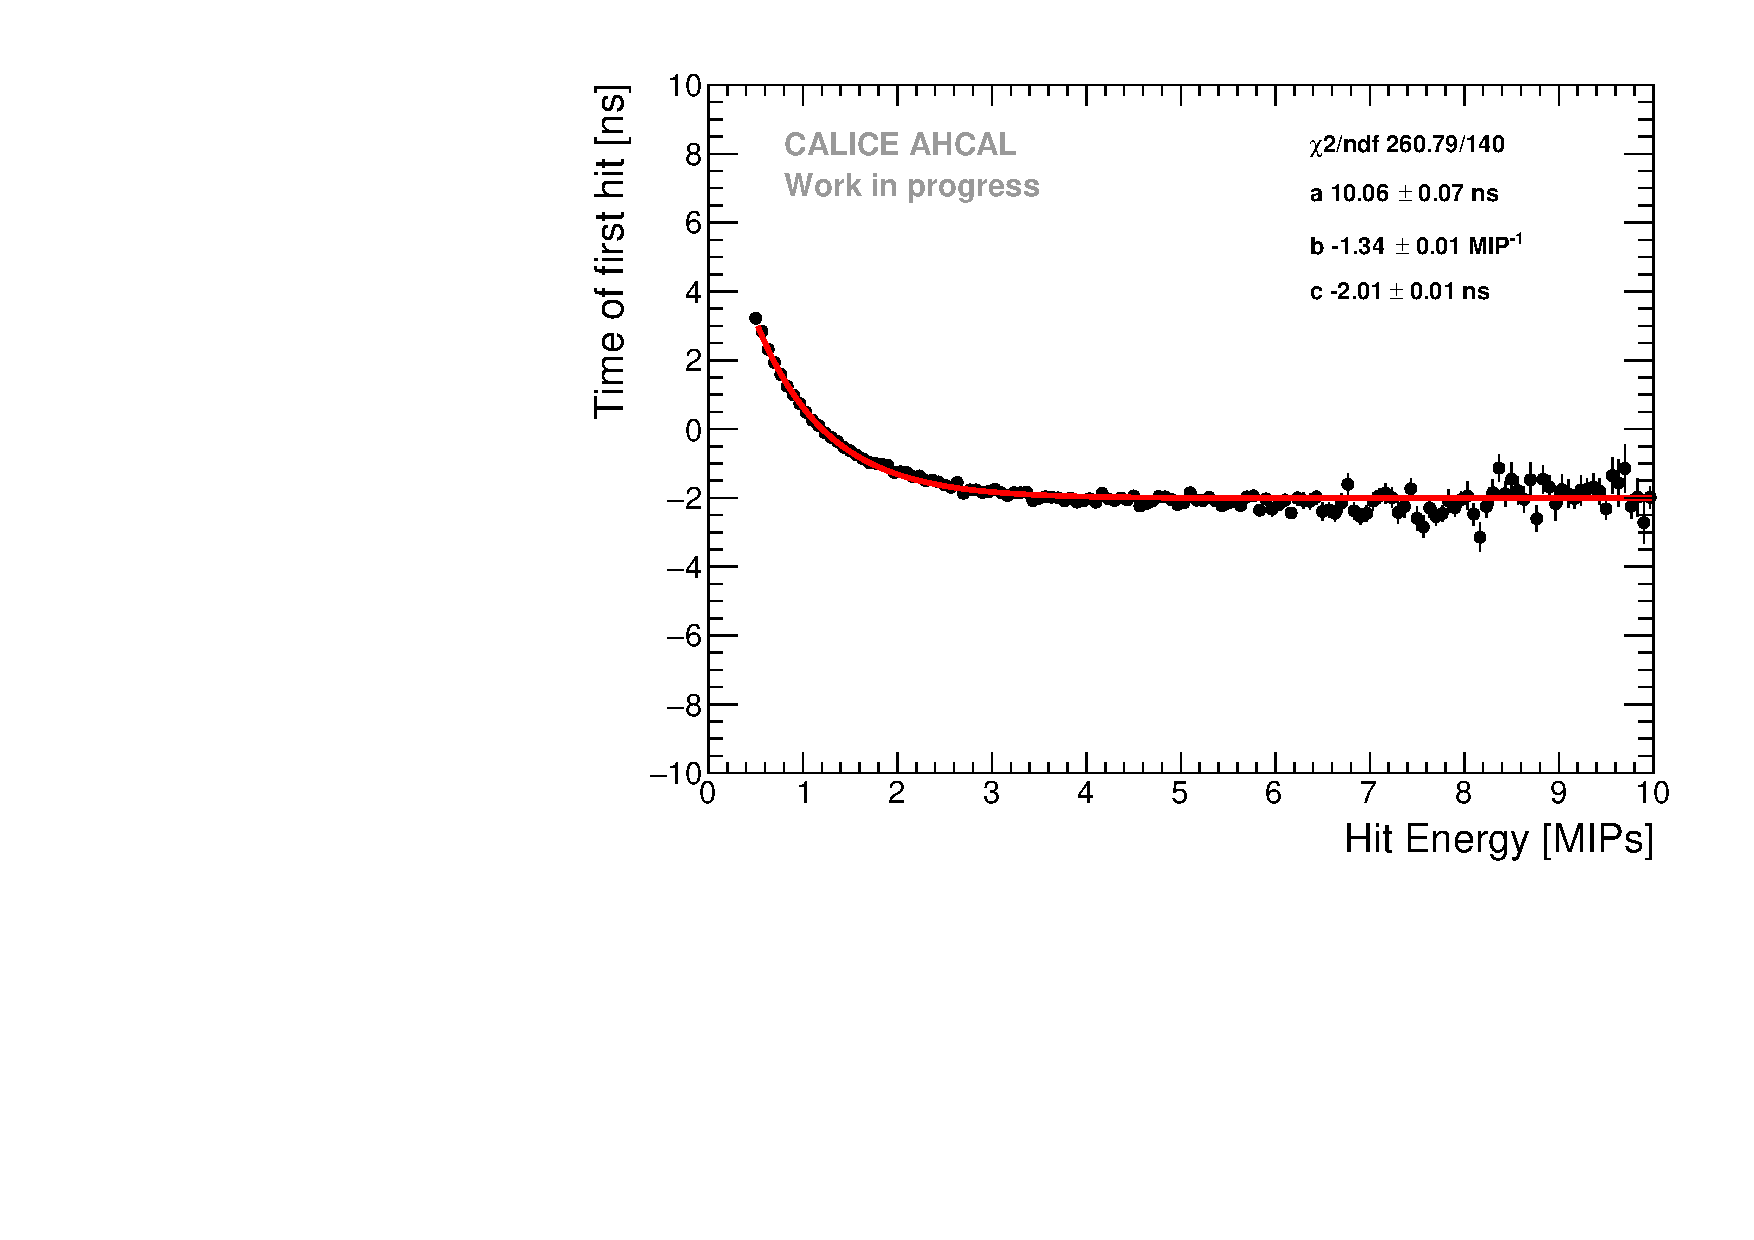
\includegraphics[width=1\textwidth]{chap5/fig_AHCAL_timing/Muons/TimeWalkProfile.pdf}
		\caption{Profile of the time of first hit as function of the hit energy.}\label{fig:time_walk}
	\end{subfigure}
	\hfill
	\begin{subfigure}[t]{0.5\textwidth}
		\centering
		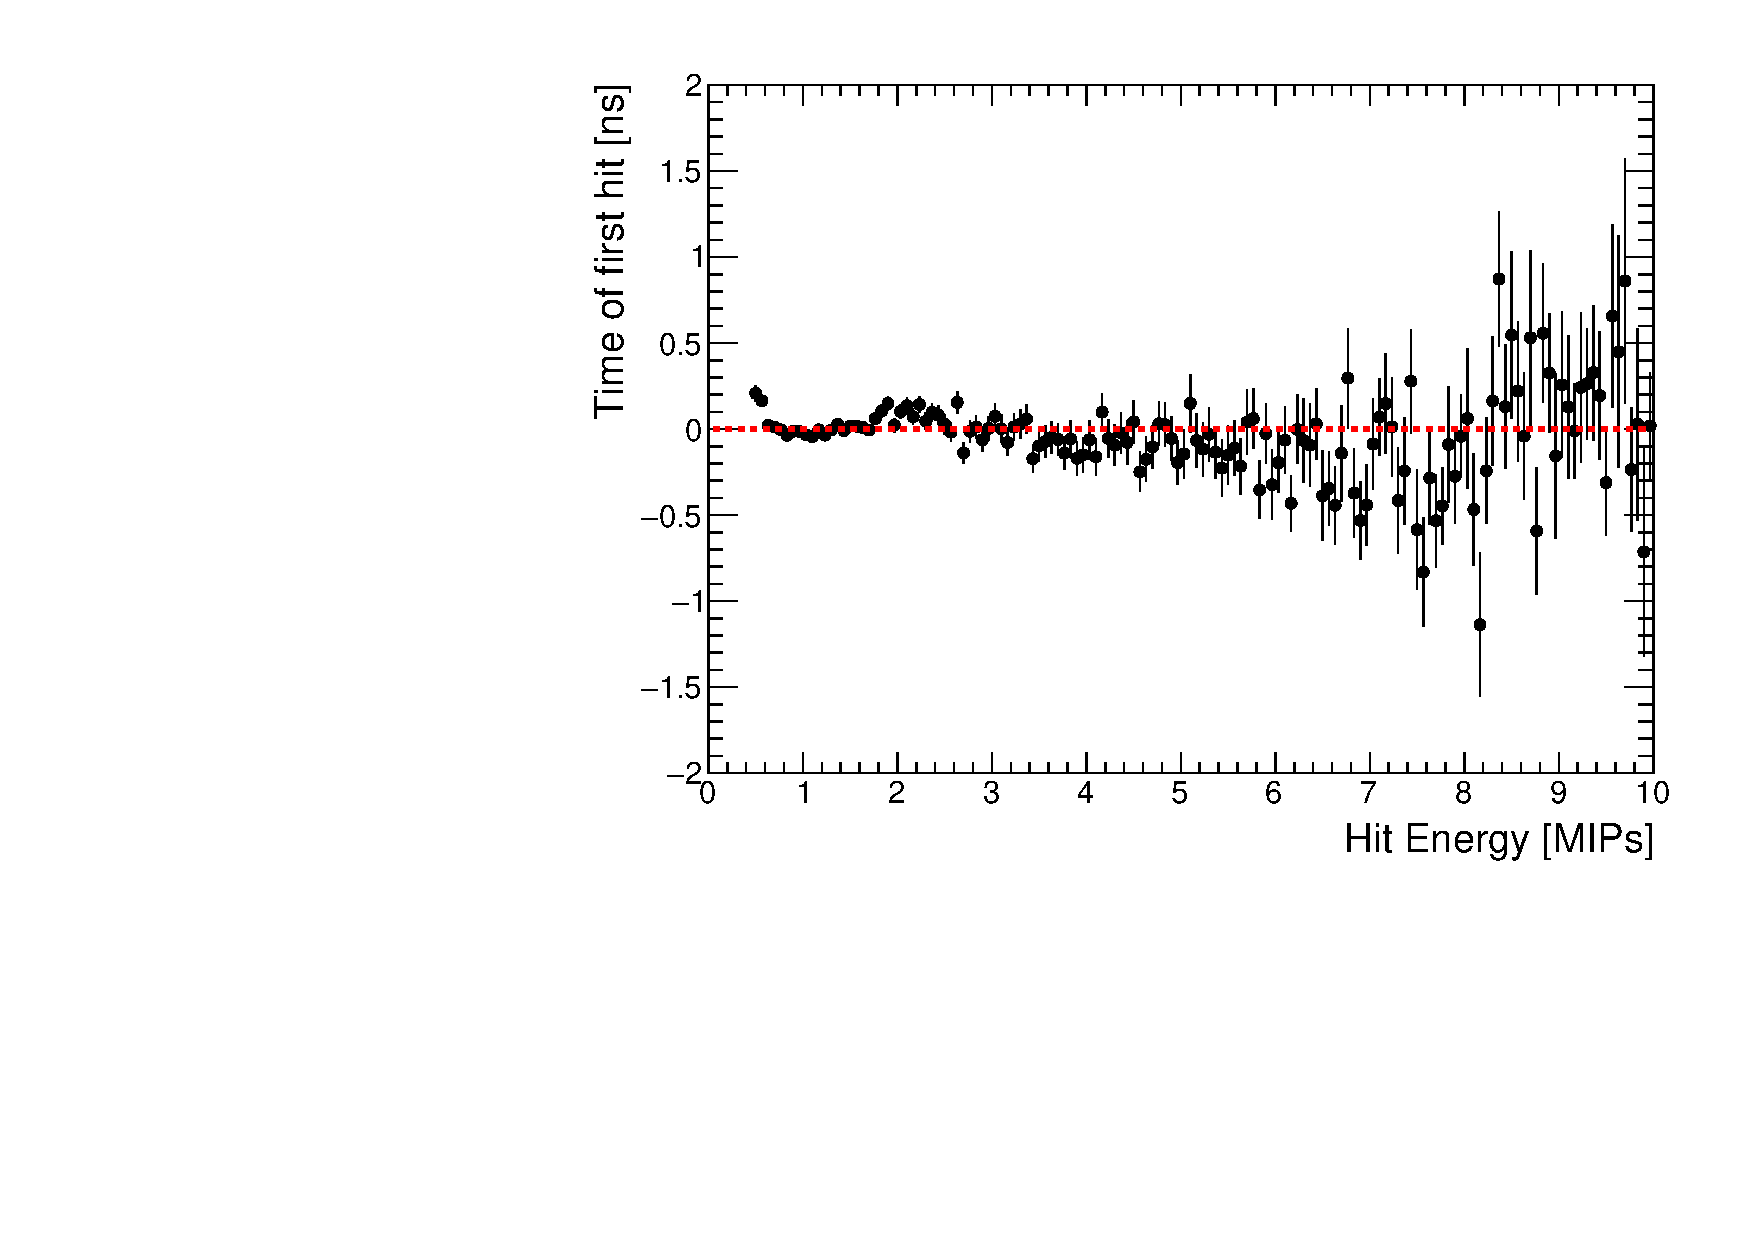
\includegraphics[width=1\textwidth]{chap5/fig_AHCAL_timing/Muons/TimeWalkProfile_Correction.pdf}
		\caption{Same profile after time-walk correction.}\label{fig:time_walk_corr}
	\end{subfigure}
	\caption{\subref{fig:time_walk}) Time-walk correction extracted from data. A = 10.06 $\pm$ 0.07, $\lambda$ = -1.34 $\pm$ 0.01, B = -2.01 $\pm$ 0.01. A difference up to 6 ns is seen between small and large amplitudes. \subref{fig:time_walk_corr}) Time-walk profile after correction showing a spread of less than 1 ns.}
\end{figure}

\subsubsection{Time of first hit for muons after corrections}
\label{subsec:Muon_final}

After the time-walk correction, an improvement of around 3\% can be achieved on the time resolution of the AHCAL as shown in figure \ref{fig:timing_muons}. The figure \ref{fig:timing_reso_all_muons} shows the time resolution obtained in the complete AHCAL. The obtained time resolution is around 5.2 ns. The distribution is still asymmetric and it is taken into account in the simulation by parametrising the time distribution with a double Gaussian function. The number of events identified later than 5$\sigma$ ($\sim$ 25 ns) is around 1.22\% giving us a good assessment of the noise suppression for muons.

\begin{figure}[htbp!]
	\begin{subfigure}[t]{0.5\textwidth}
		\centering
		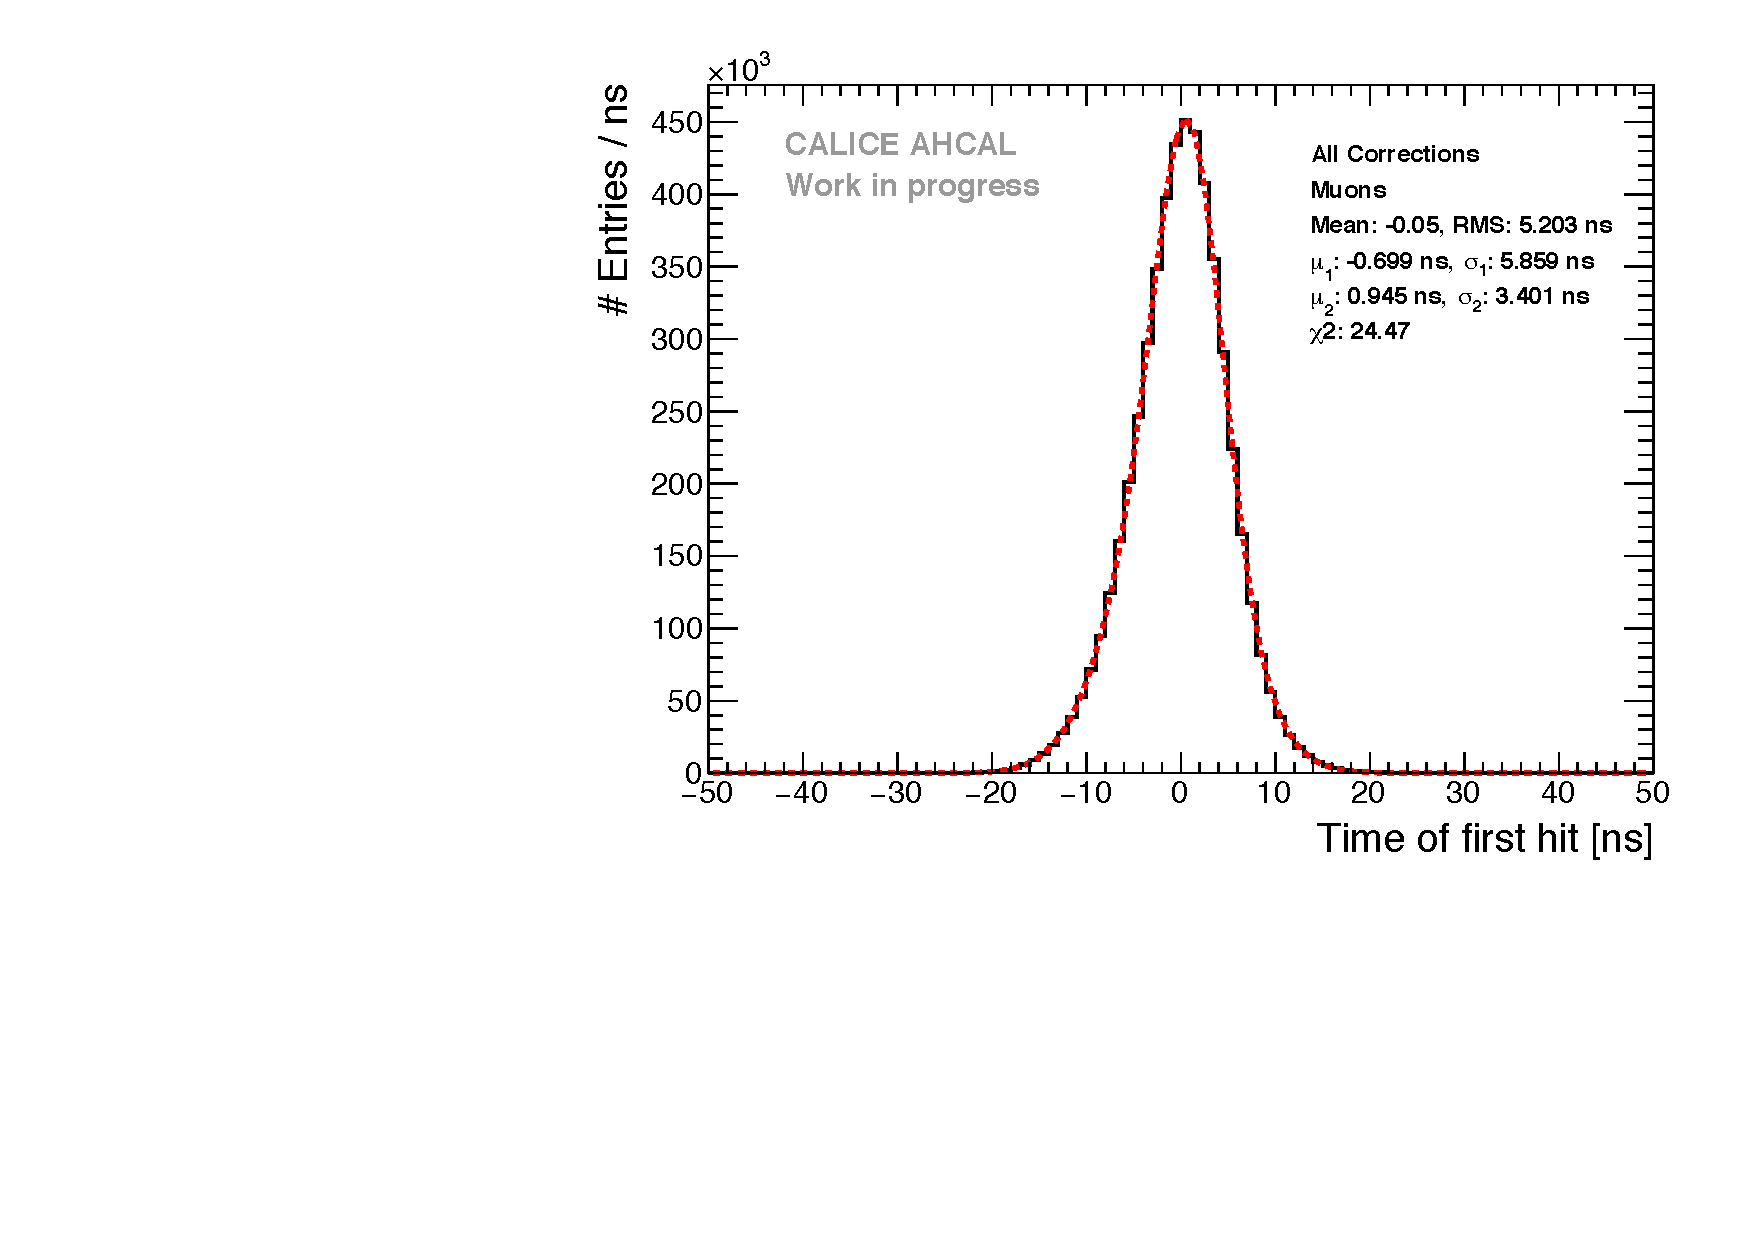
\includegraphics[width=1\textwidth]{chap5/fig_AHCAL_timing/Muons/Timing_AllLayers.pdf}
		\caption{Time of the first hit distribution of the AHCAL after all corrections.}\label{fig:timing_muons}
	\end{subfigure}
	\hfill
	\begin{subfigure}[t]{0.5\textwidth}
		\centering
		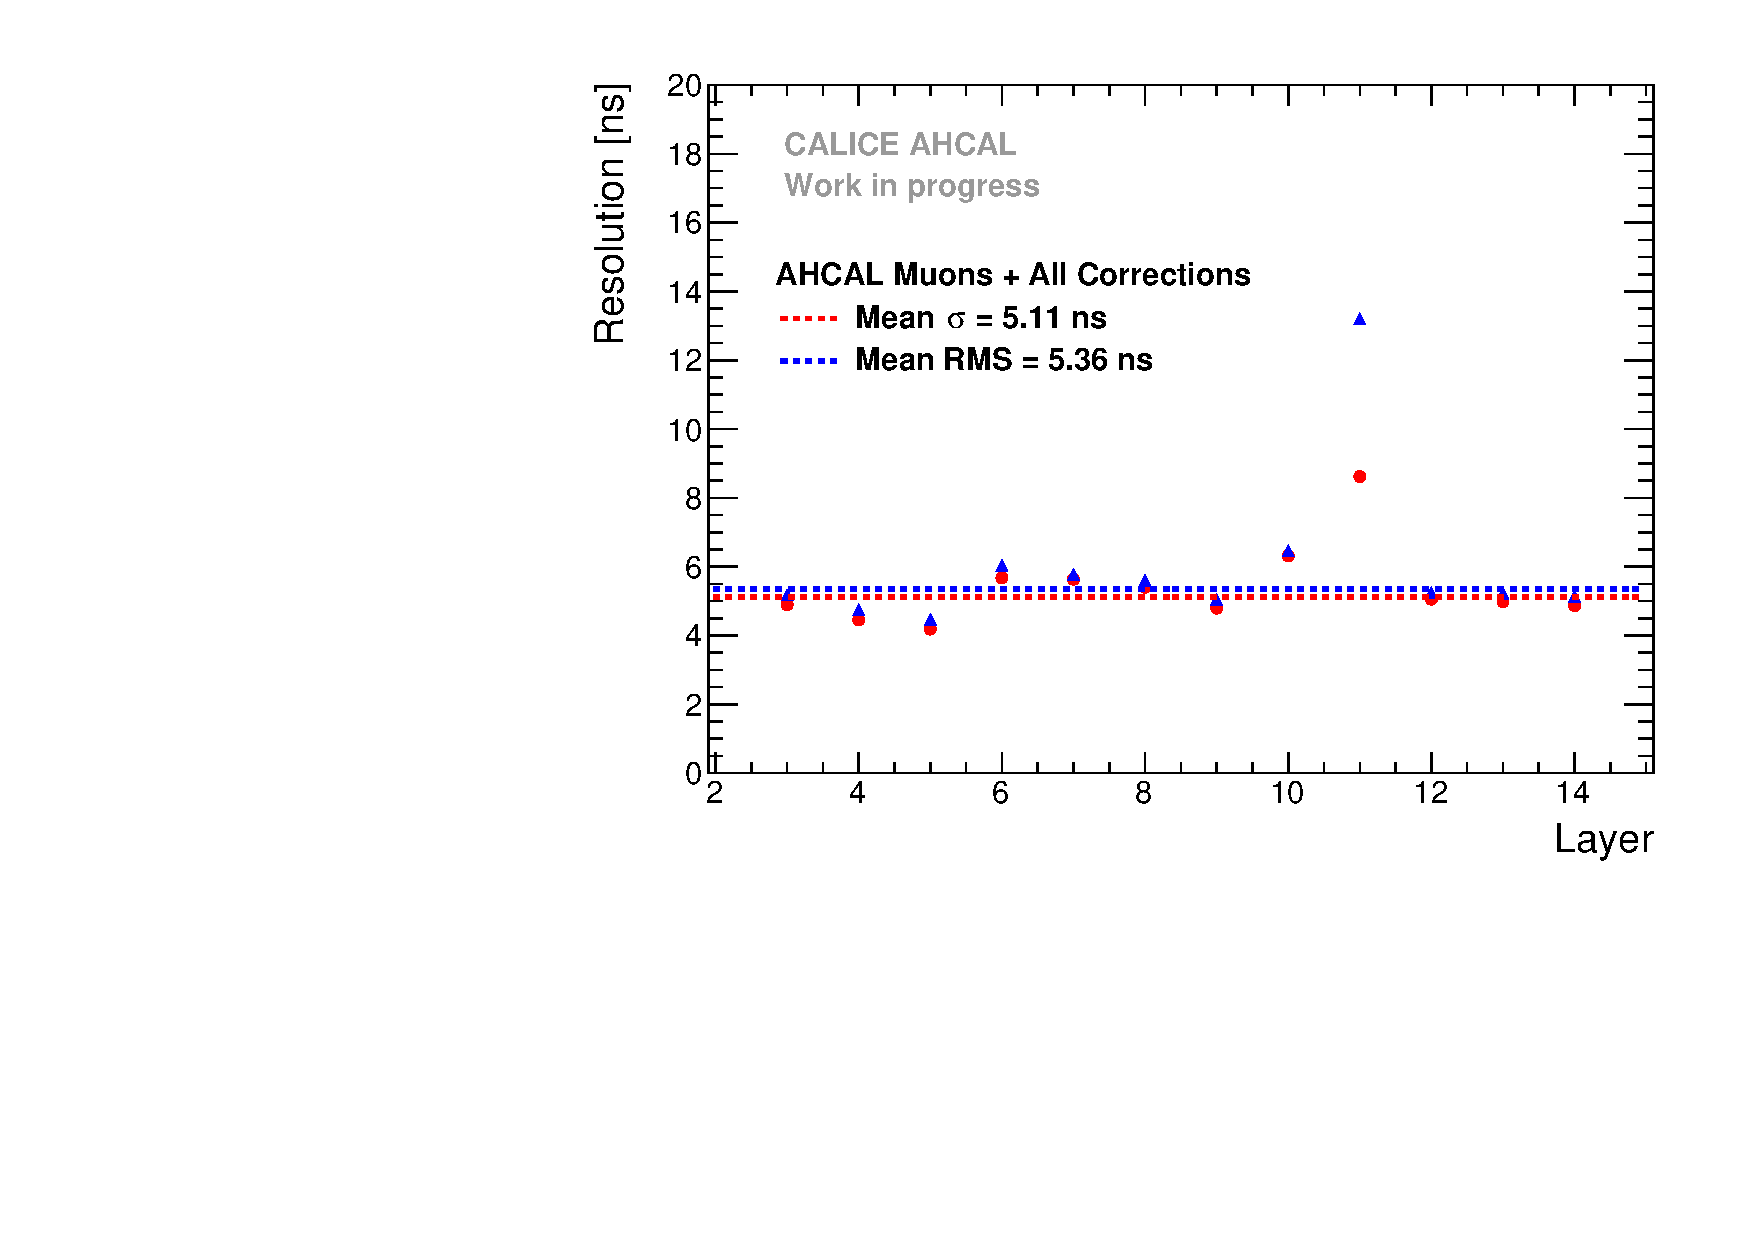
\includegraphics[width=1\textwidth]{chap5/fig_AHCAL_timing/Muons/ResolutionPerModule_AllCorrection.pdf}
		\caption{Time resolution obtained for each AHCAL layers.}\label{fig:timing_reso_all_muons}
	\end{subfigure}
	\caption{\subref{fig:timing_muons}) Time of the first hit for muons after all corrections excluding layer 11. The extracted parameters are then used to tune the simulation. \subref{fig:timing_reso_all_muons}) Time resolution obtained for each layer in the AHCAL. Mean RMS = 5.35 ns.}
\end{figure}

After all corrections, the time resolution obtained is far from the 1 ns time resolution desired which is most likely due to the domination in the time resolution of the time reference which is around 4-5 ns. Assuming that it is a simple convolution of the time resolution of the AHCAL and the resolution of the time reference (around 4-5 ns), then the AHCAL time resolution would be around $\sigma_{AHCAL} \sim \sqrt{\sigma_{t}^2 - \sigma_{Tref}^2} \sim$ 2.6 ns which is consistant with previous measurements of single channel time resolution \cite{Laurien2016}.

\subsection{Cross-check of the calibration with electrons}
\label{subsec:validation}

In order to validate the calibration, an electron sample is taken. Electromagnetic showers are quasi-instantaneous and perfect to cross-check the time calibration procedure. The selection applied to the data sample is described in subsection \ref{subsec:elec_sel}. The same calibration constants and correction constants are applied to the data except that an additional offset from the trigger signal has to be corrected for.

The additional offset is expected to be small as the trigger configuration is very similar to the one for muons. The offset is in the order of 10 ns which is consistent with the changes in trigger configuration from the big scintillator plates to the small trigger scintillator of $10\times10$ cm$^2$. The time of the first hit distribution is shown in figure \ref{fig:Timing_electrons}. The time distribution presents a large tail to the right and is much wider than for muons. This gives a hint that an effect is present in electron data but not in muon data. The difference seen could be related to the fact that in electromagnetic showers, the number of hits is much higher as well as the energy deposited in a single cell can be over hundreds MIP.

\begin{figure}[htbp!]
	\centering
	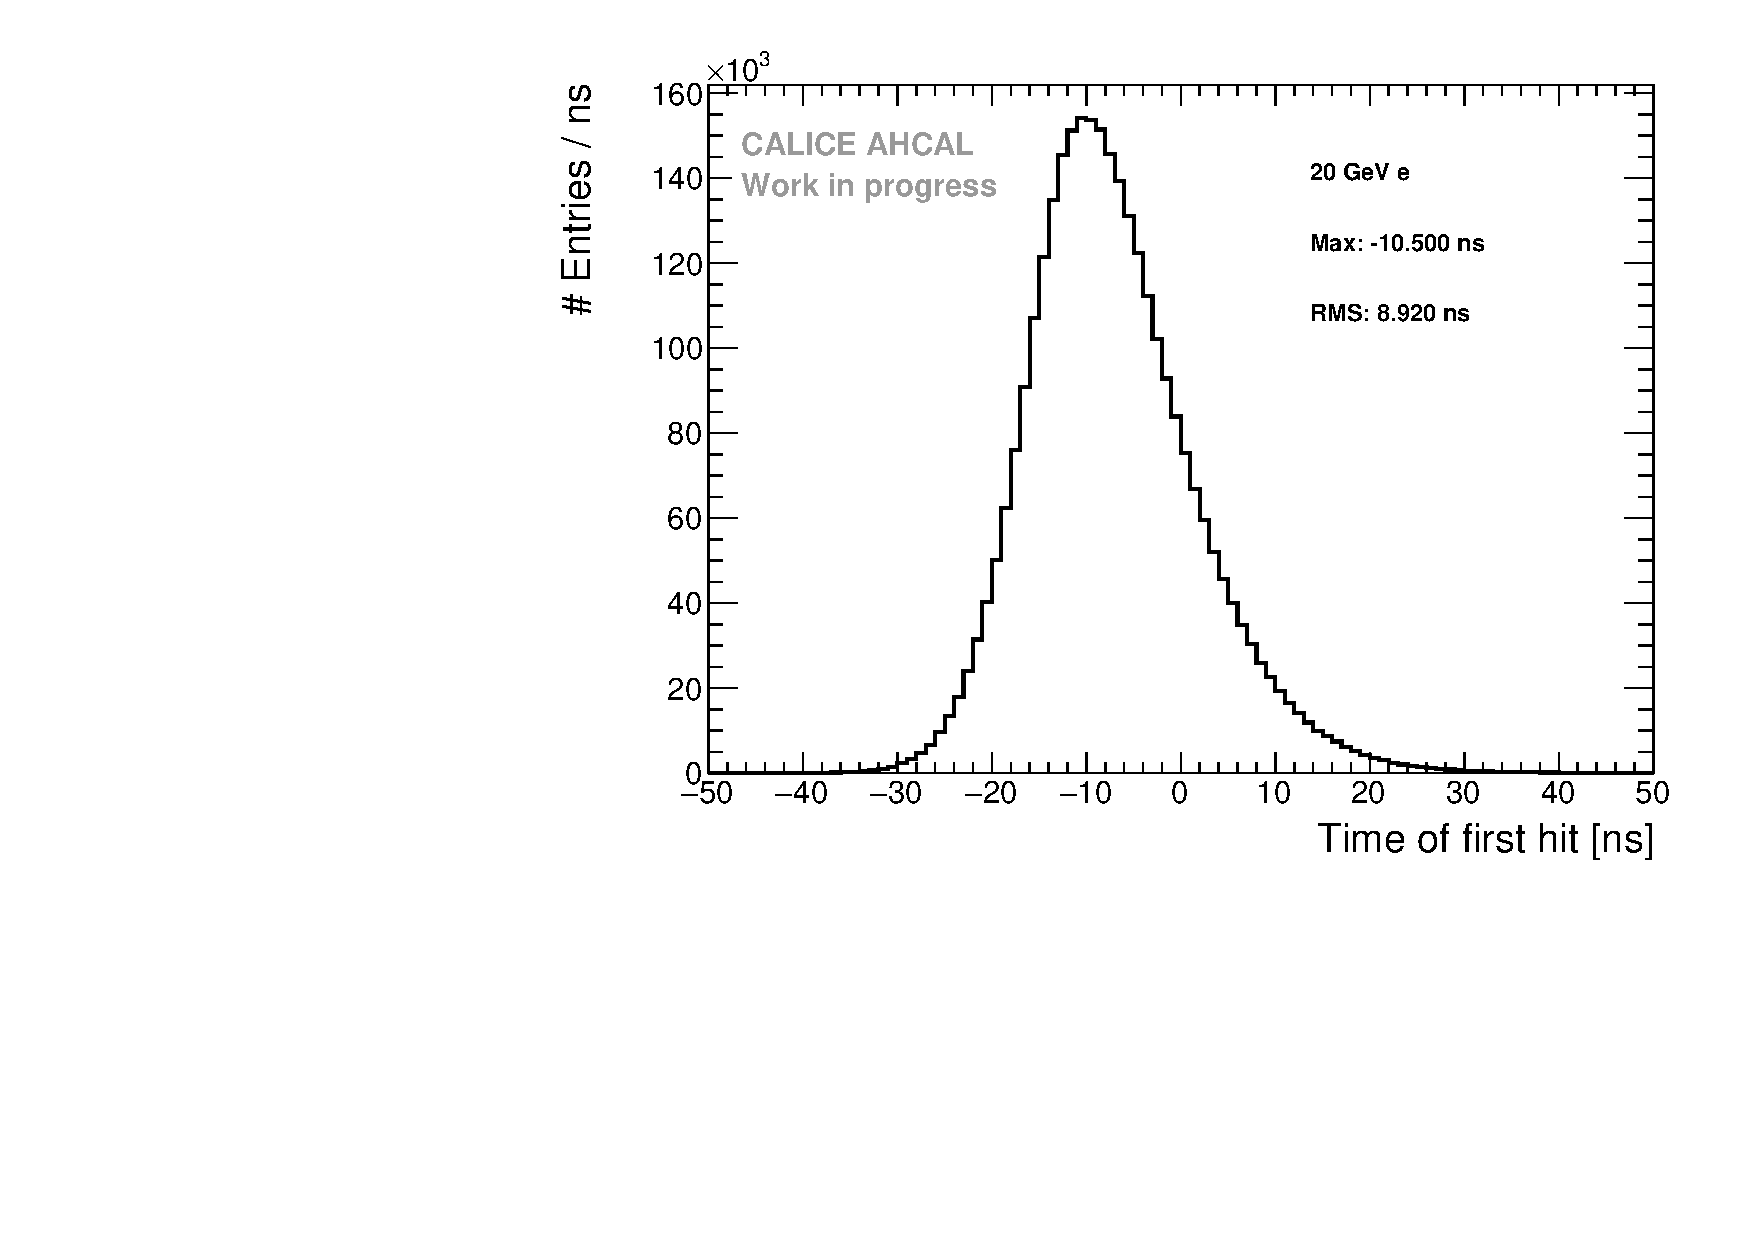
\includegraphics[width=0.6\textwidth]{chap5/fig_AHCAL_timing/Electrons/Timing_AllLayers_AfterMuons.pdf}
	\caption{Time of the first hit distribution for 20 GeV electrons, Max = -10.05 ns, RMS = 8.92 ns.}
	\label{fig:Timing_electrons}
\end{figure}

\subsection{Influence of the number of triggered channels}
\label{subsec:ped_shift}

Pedestal shift for energy measurement is not a new feature of the \textit{SPIROC2B} chip \cite{Hartbrich2012}. This electronic effect may be also present for timing measurement. It can be investigated by looking at the time of the first hit as a function of the number of triggered channels over 0.5 MIP. The correction should not be energy dependant and all electron energies is used to determine the correction curve.

It is shown in figure \ref{fig:nhits_profile}. This can be drastic on the time measurement of the AHCAL, a correction up to 30-40 ns can be necessary to the data for a high number of trigger (15-20). The correction parameters are determined by a polynomial fit to the data. In addition, this effect does not only shift the mean of the time distribution but as well increases its width. The width increases with the number of triggers in a chip thus making the time resolution of the AHCAL dependant on the number of hits. This is shown in figure \ref{fig:RMS_nHits}. As expected, if only a single channel triggers in a chip, the time resolution is closed to the one obtained for muons.

\begin{figure}[htbp!]
	\begin{subfigure}[t]{0.5\textwidth}
		\centering
		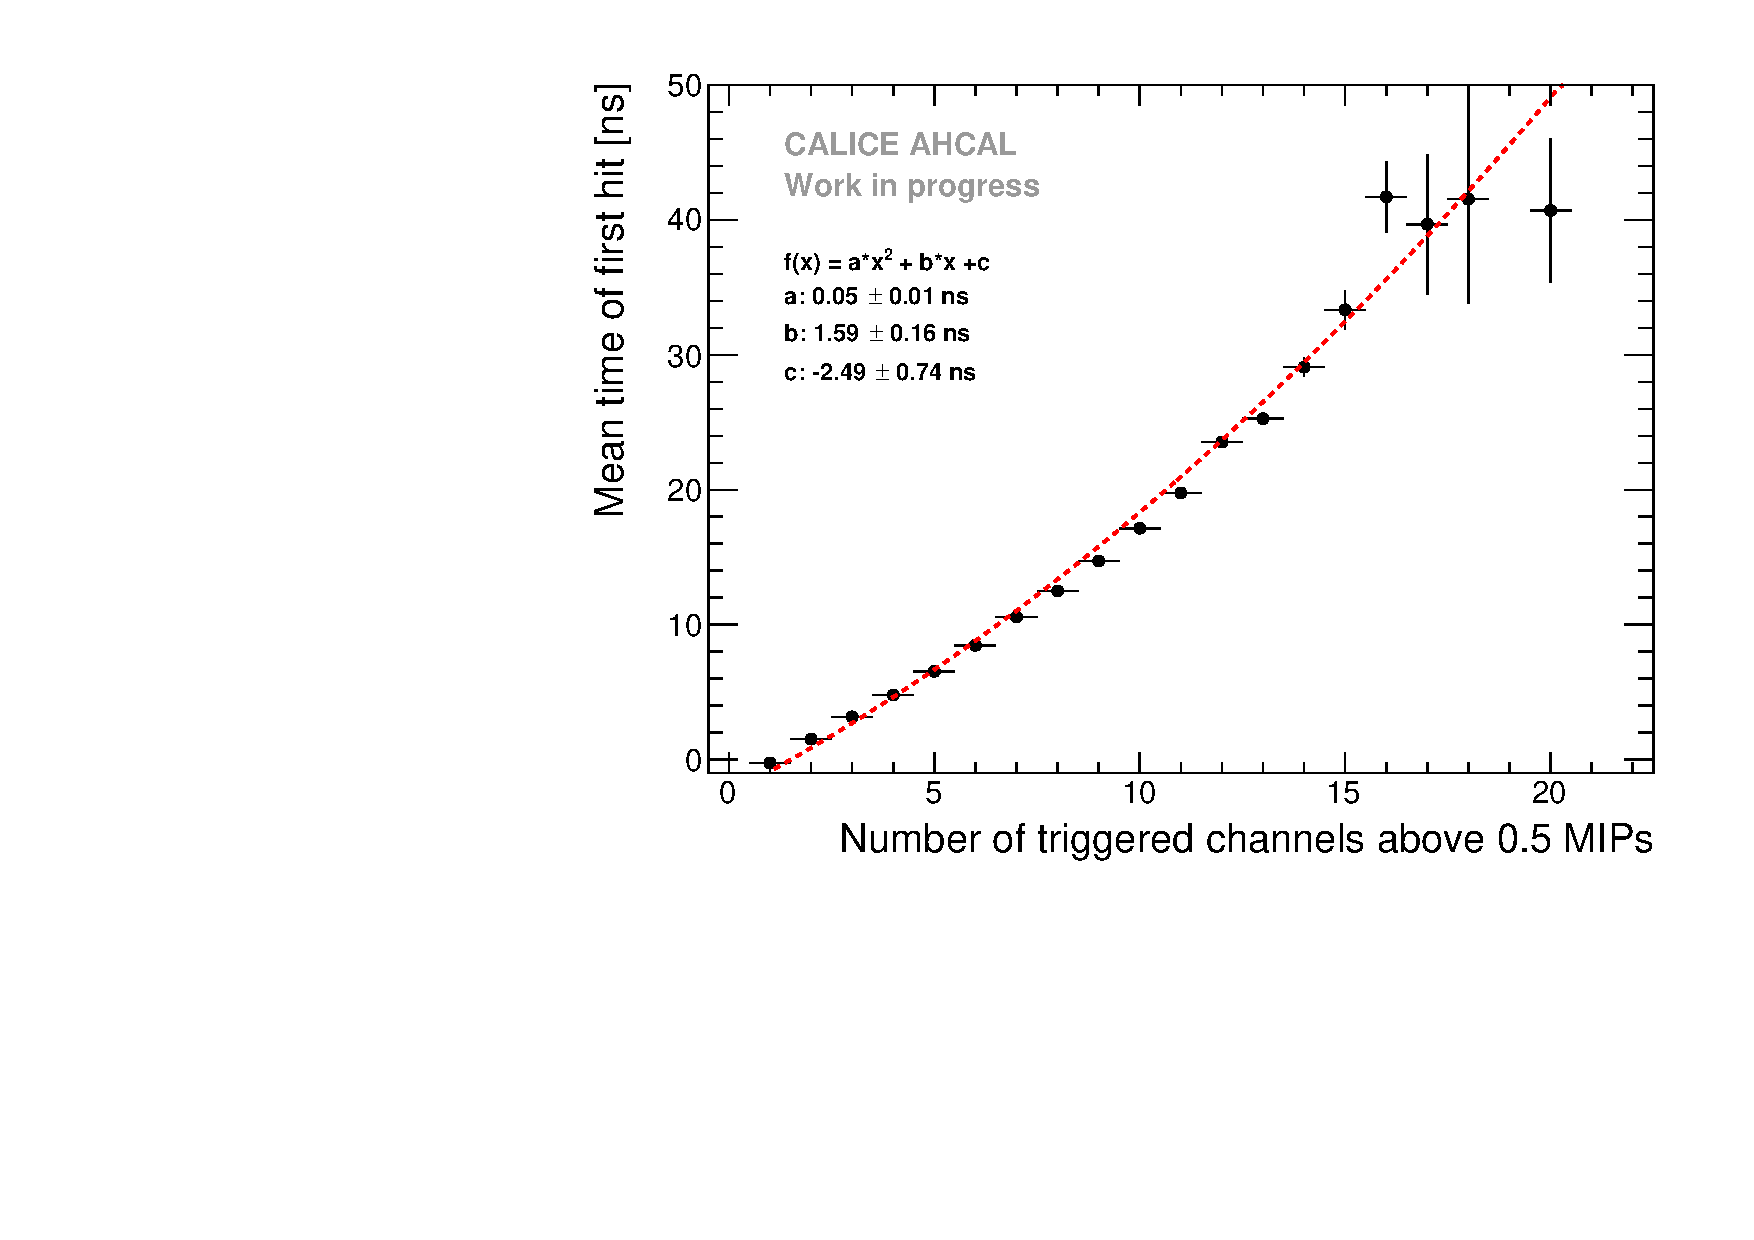
\includegraphics[width=1\textwidth]{chap5/fig_AHCAL_timing/Electrons/NumberHits_Dependance_AllEnergies.pdf}
		\caption{Time of the first hit function of the number of triggered channels in a chip for all electron energies.}\label{fig:nhits_profile}
	\end{subfigure}
	\hfill
	\begin{subfigure}[t]{0.5\textwidth}
		\centering
		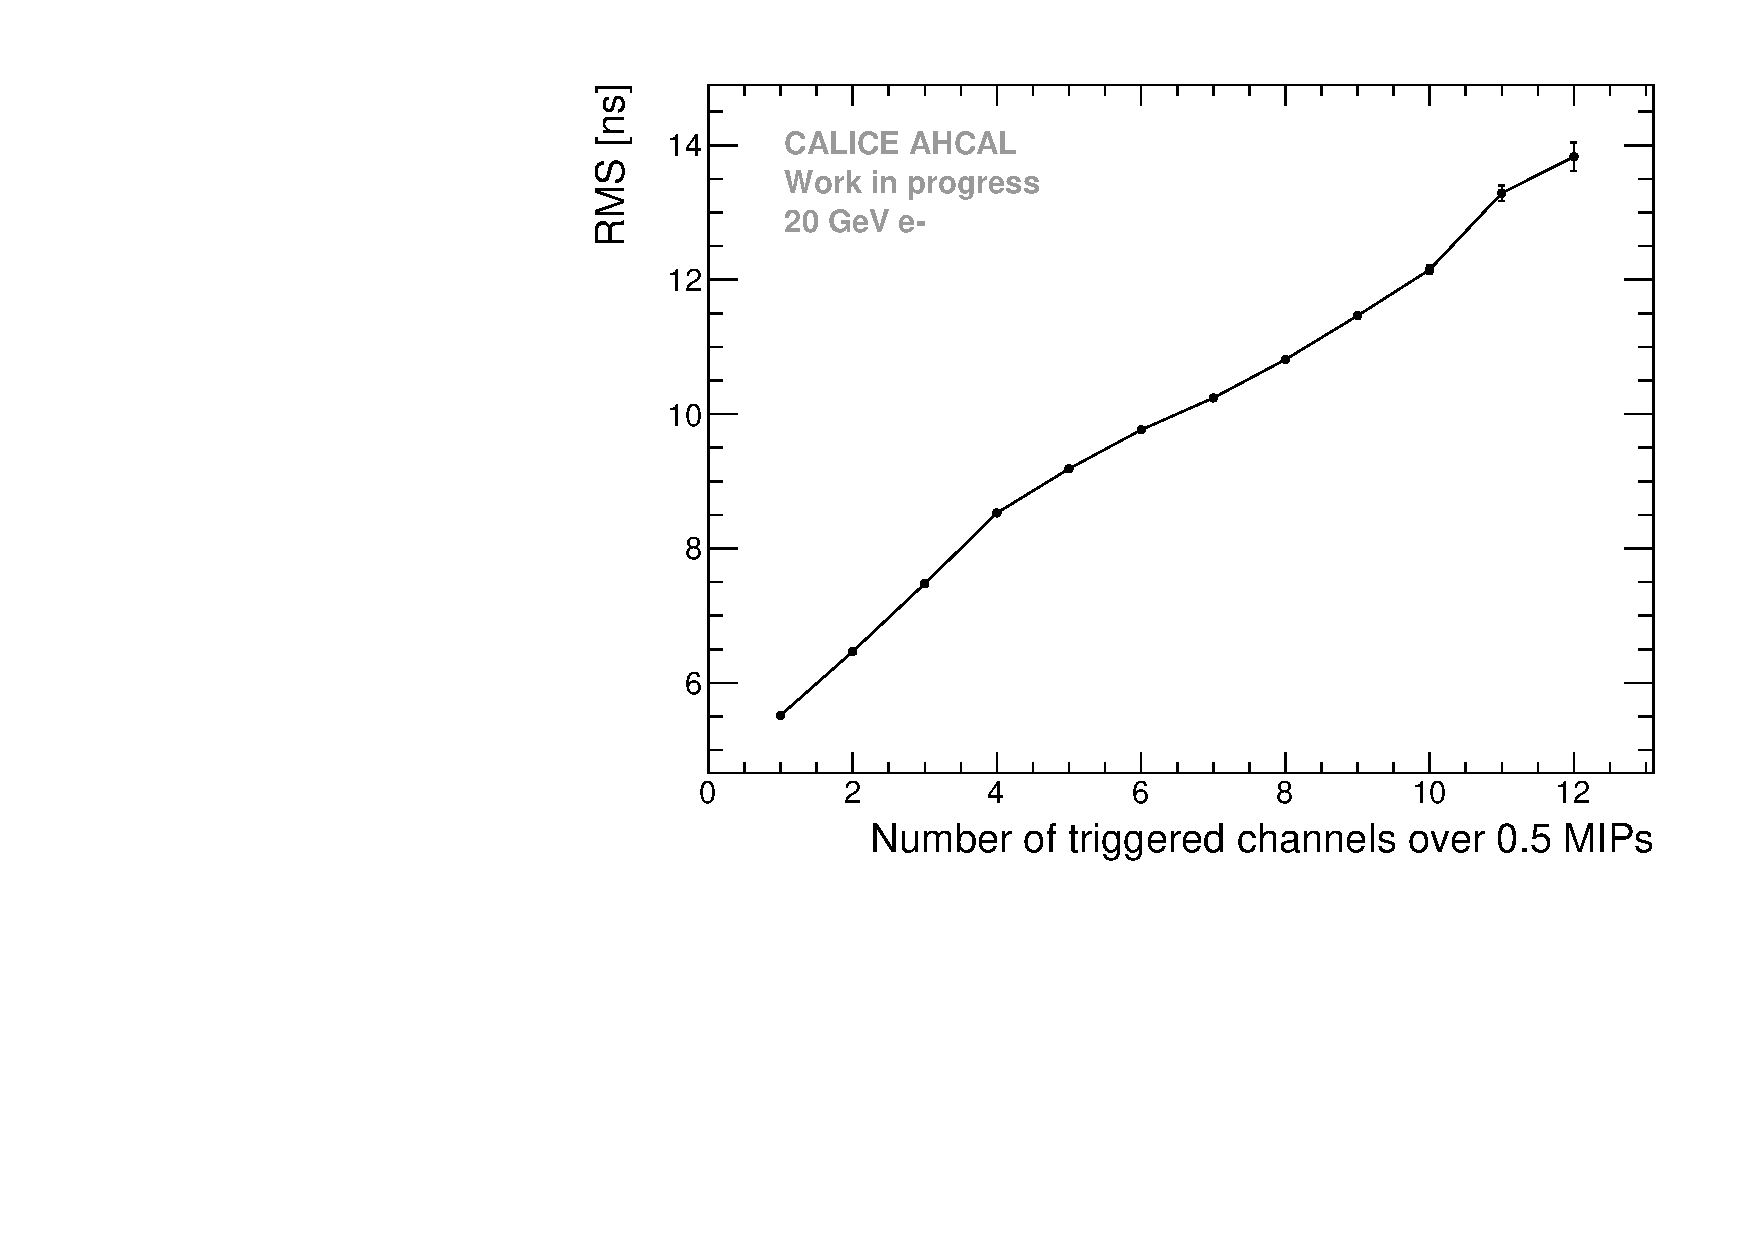
\includegraphics[width=1\textwidth]{chap5/fig_AHCAL_timing/Electrons/ParametrisationPedestalShift_20GeV.pdf}
		\caption{RMS of the time of first hit function of the number of triggered channels for 20 GeV electrons.}\label{fig:RMS_nHits}
	\end{subfigure}
	\caption{\subref{fig:nhits_profile}) Mean time of the hit as function of the number of triggered channels in a chip. The mean time shift upwards with the increase of triggers leading to large tails in the time distribution. The plot is obtained by combining all electron energies and a polynomial fit is done. \subref{fig:RMS_nHits}) The RMS of the time distribution can increase up to 10-15 ns for a high number of triggered channels.}
\end{figure}

\subsection{Time of the first hit for electrons}
\label{subsec:Electron_Final}

The distribution of the time of the first for 20 GeV is shown in figure \ref{fig:timing_electrons_corr} after correction as function of the triggered channels. The correction improves the RMS of the distribution, around 12.1\%, as well as the distribution appears more gaussian-like. However, there is still a discrepancy (around 33.7\%) with the time resolution obtained for muons (5.2 ns). This is due to the fact that not only the mean time shifts but that the RMS also increases as a function of number of hits as seen in figure \ref{fig:RMS_nHits} and can't be corrected. In order for the simulation to match the data, the increase of the width of the time distribution has to be parametrised from the data. More details can be read in the appendix \ref{appendix:ped_shift}.

\begin{figure}[htbp!]
	\begin{subfigure}[t]{0.5\textwidth}
		\centering
		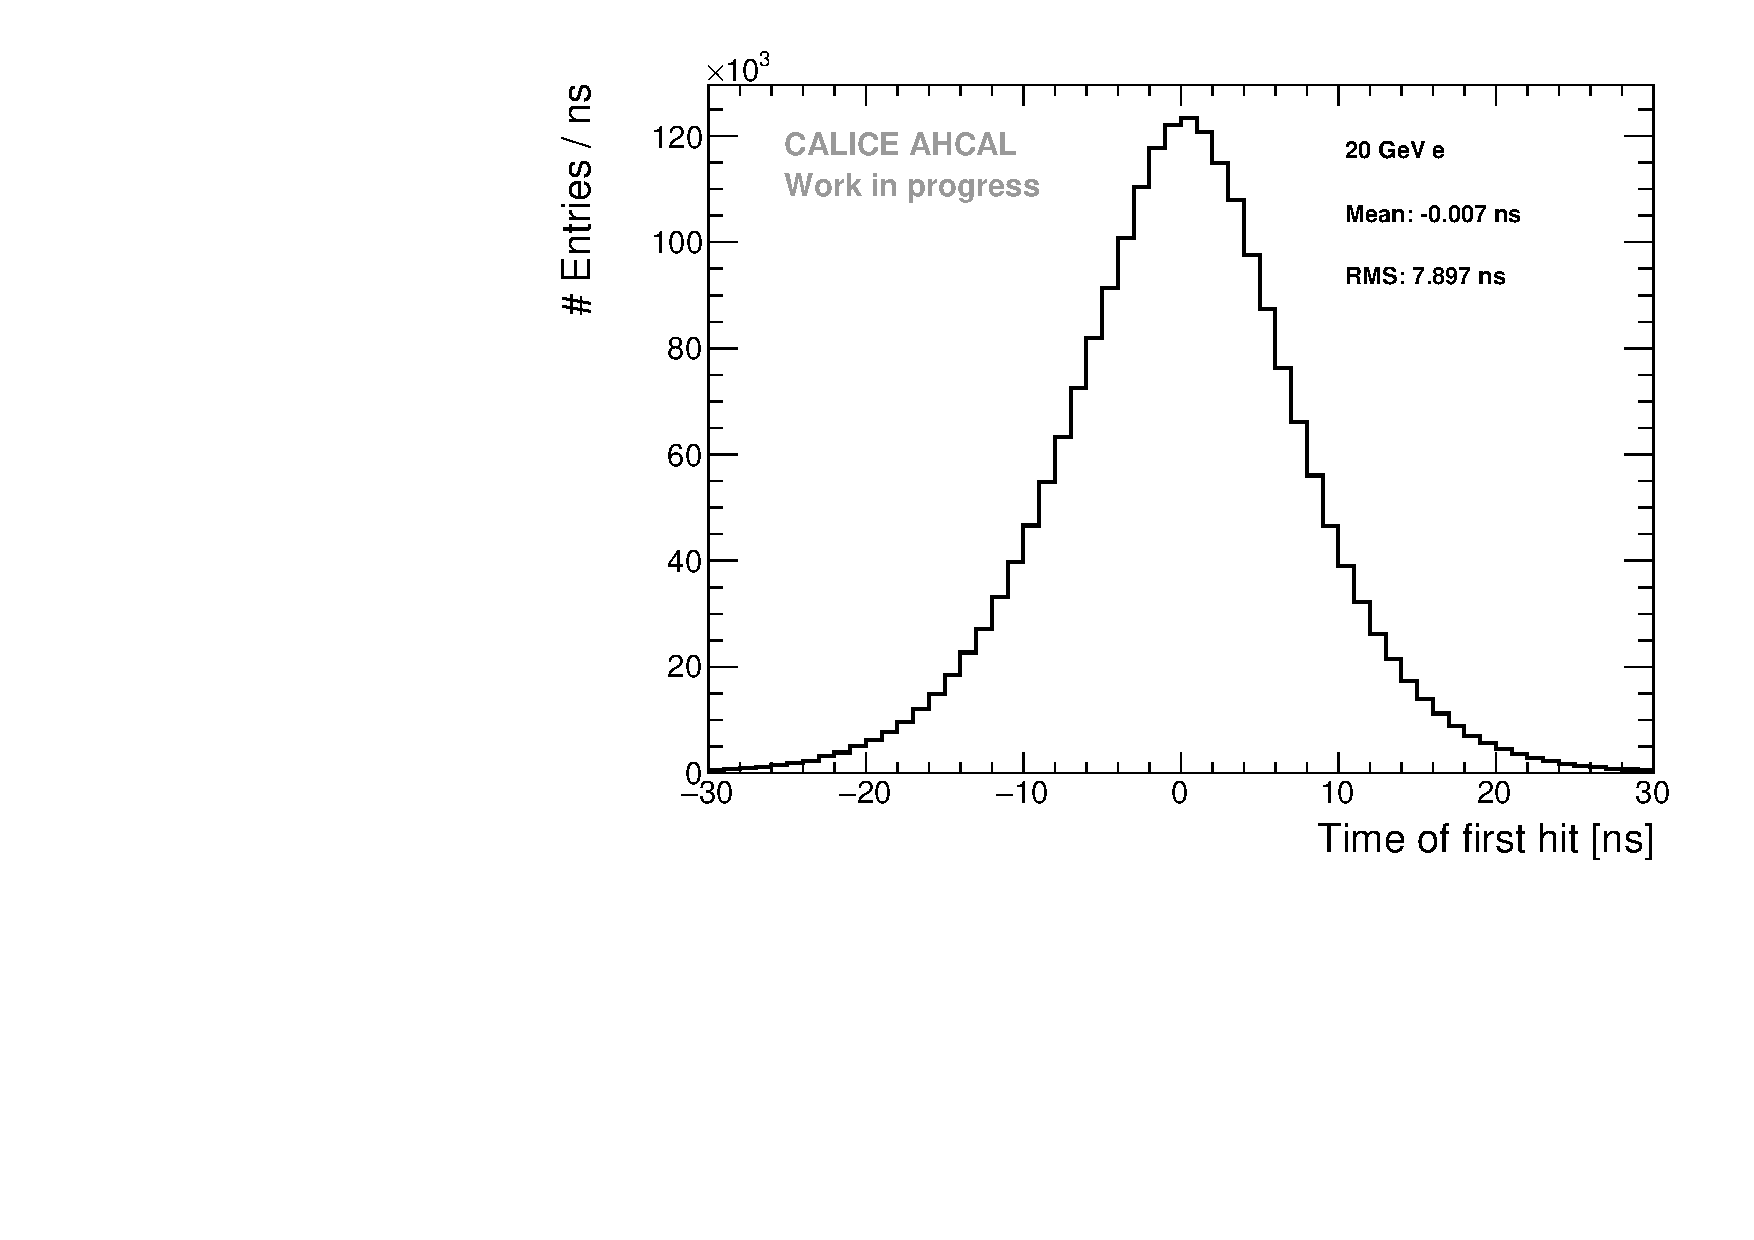
\includegraphics[width=1\textwidth]{chap5/fig_AHCAL_timing/Electrons/Timing_AllLayers_20GeV.pdf}
		\caption{Time of the first hit distribution for 20 GeV electrons after correction as function of the number of triggered channels.}\label{fig:timing_electrons_corr}
	\end{subfigure}
	\hfill
	\begin{subfigure}[t]{0.5\textwidth}
		\centering
		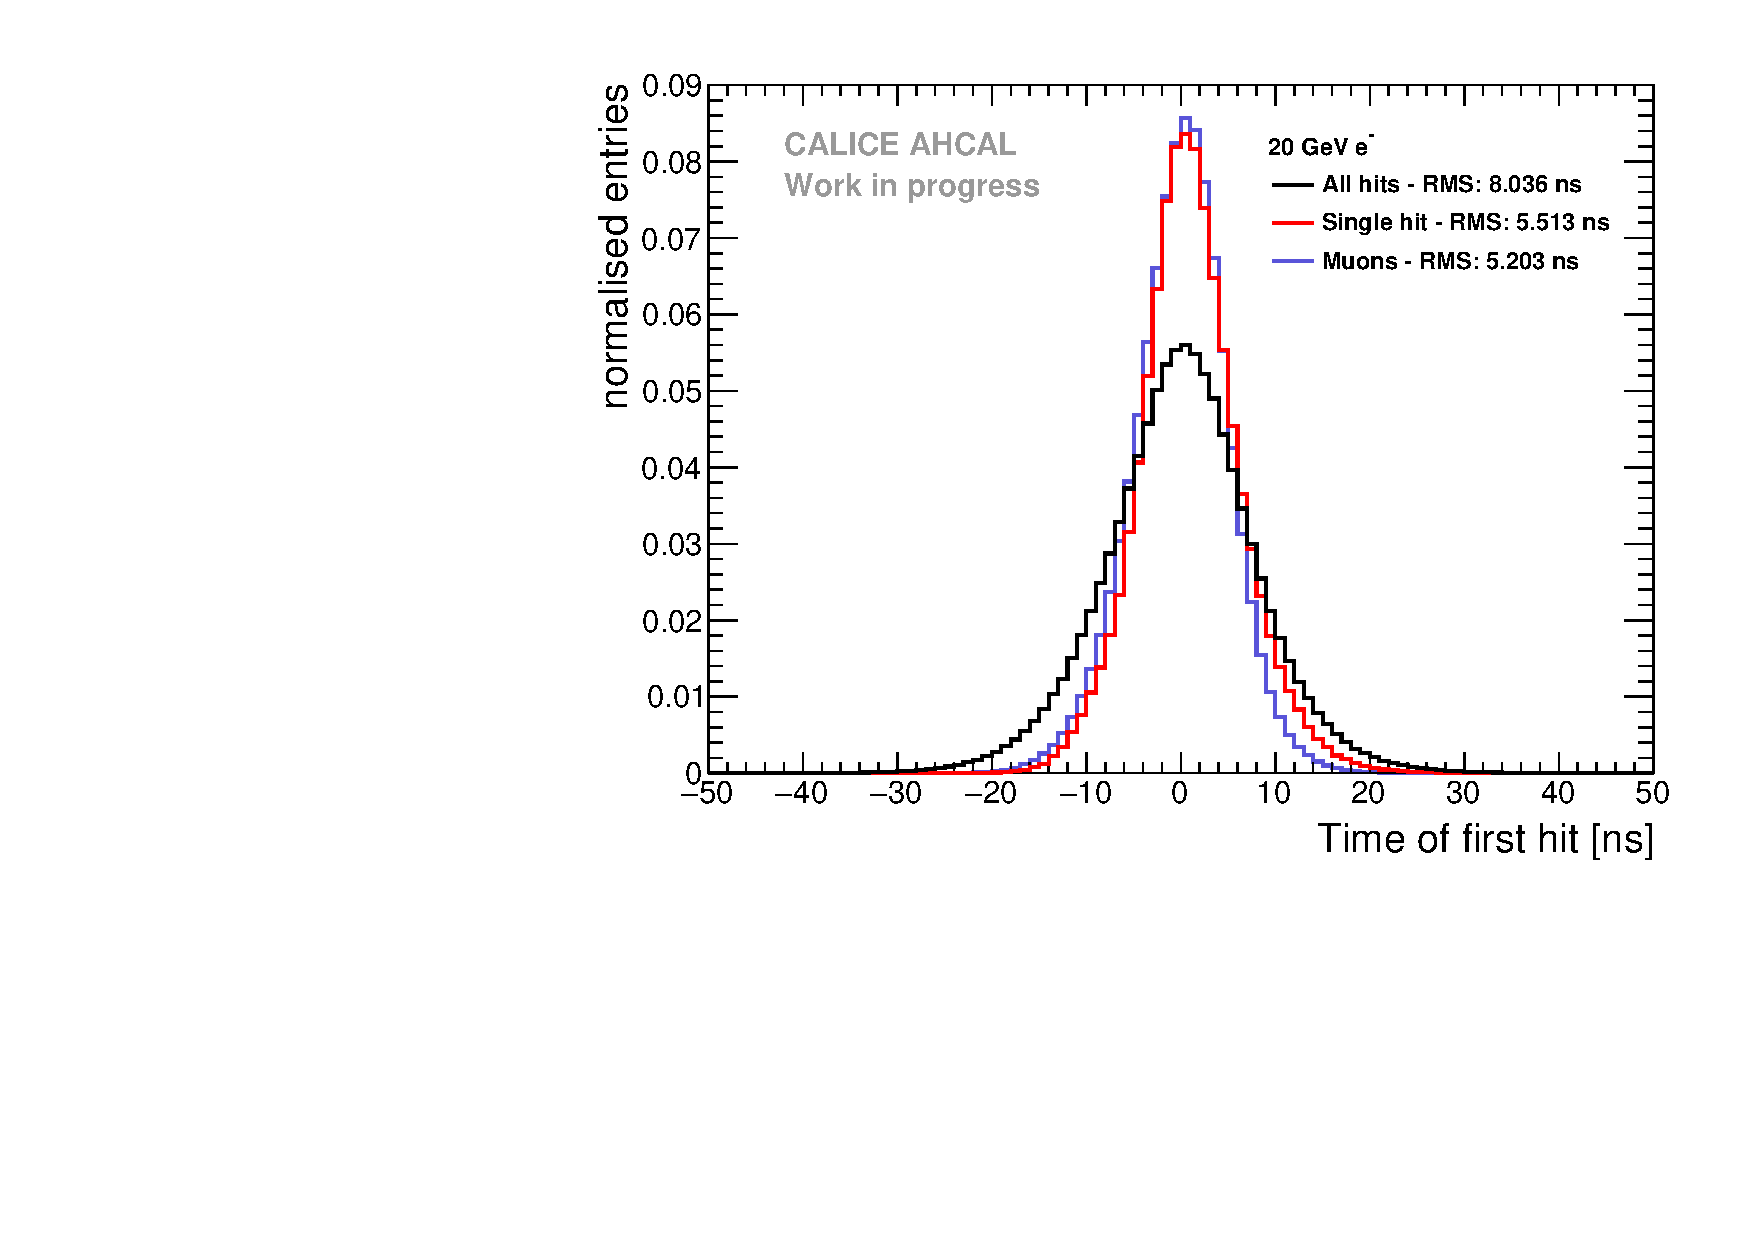
\includegraphics[width=1\textwidth]{chap5/fig_AHCAL_timing/Electrons/ComparisonAll_ElectronsSingleHit.pdf}
		\caption{Comparison between eletrons and muons of time of first hit distribution.}\label{fig:timing_electron_muon_comp}
	\end{subfigure}
	\caption{\subref{fig:timing_electrons_corr}) Time of the first hit distribution for 20 GeV electrons after number of triggered channel correction, $\mu$ = -0.018 ns, RMS = 7.84 ns. \subref{fig:timing_electron_muon_comp}) Comparison of the electron data sample, the time distribution is very similar to the muon one if only events with single hits in a chip are taken.}
\end{figure}

A comparison with the muon data has been done in order to cross-check the calibration as well as the correction as seen in figure \ref{fig:timing_electron_muon_comp}. If only single hits in a chip are taken, the time resolution obtained is very similar to the time resolution observed in muons (around 5.2\% difference). The cause of observed effect is most likely due to an element in the chip called a delay box that get unstable with the number of triggered channels and that is responsible for the hold of the TDC value in the chip. The hold is delayed thus the sampling of a higher TDC value than the one expected is done.

All electron runs have been checked to validate the correction and calibration procedure. The figure \ref{fig:all_electron_energies} shows the comparison from 10 GeV to 50 GeV. The distributions are in agreement for all energies within systematical uncertainty as explained in subsection \ref{subsec:det_inhomo}.

\begin{figure}[htbp!]
	\centering
	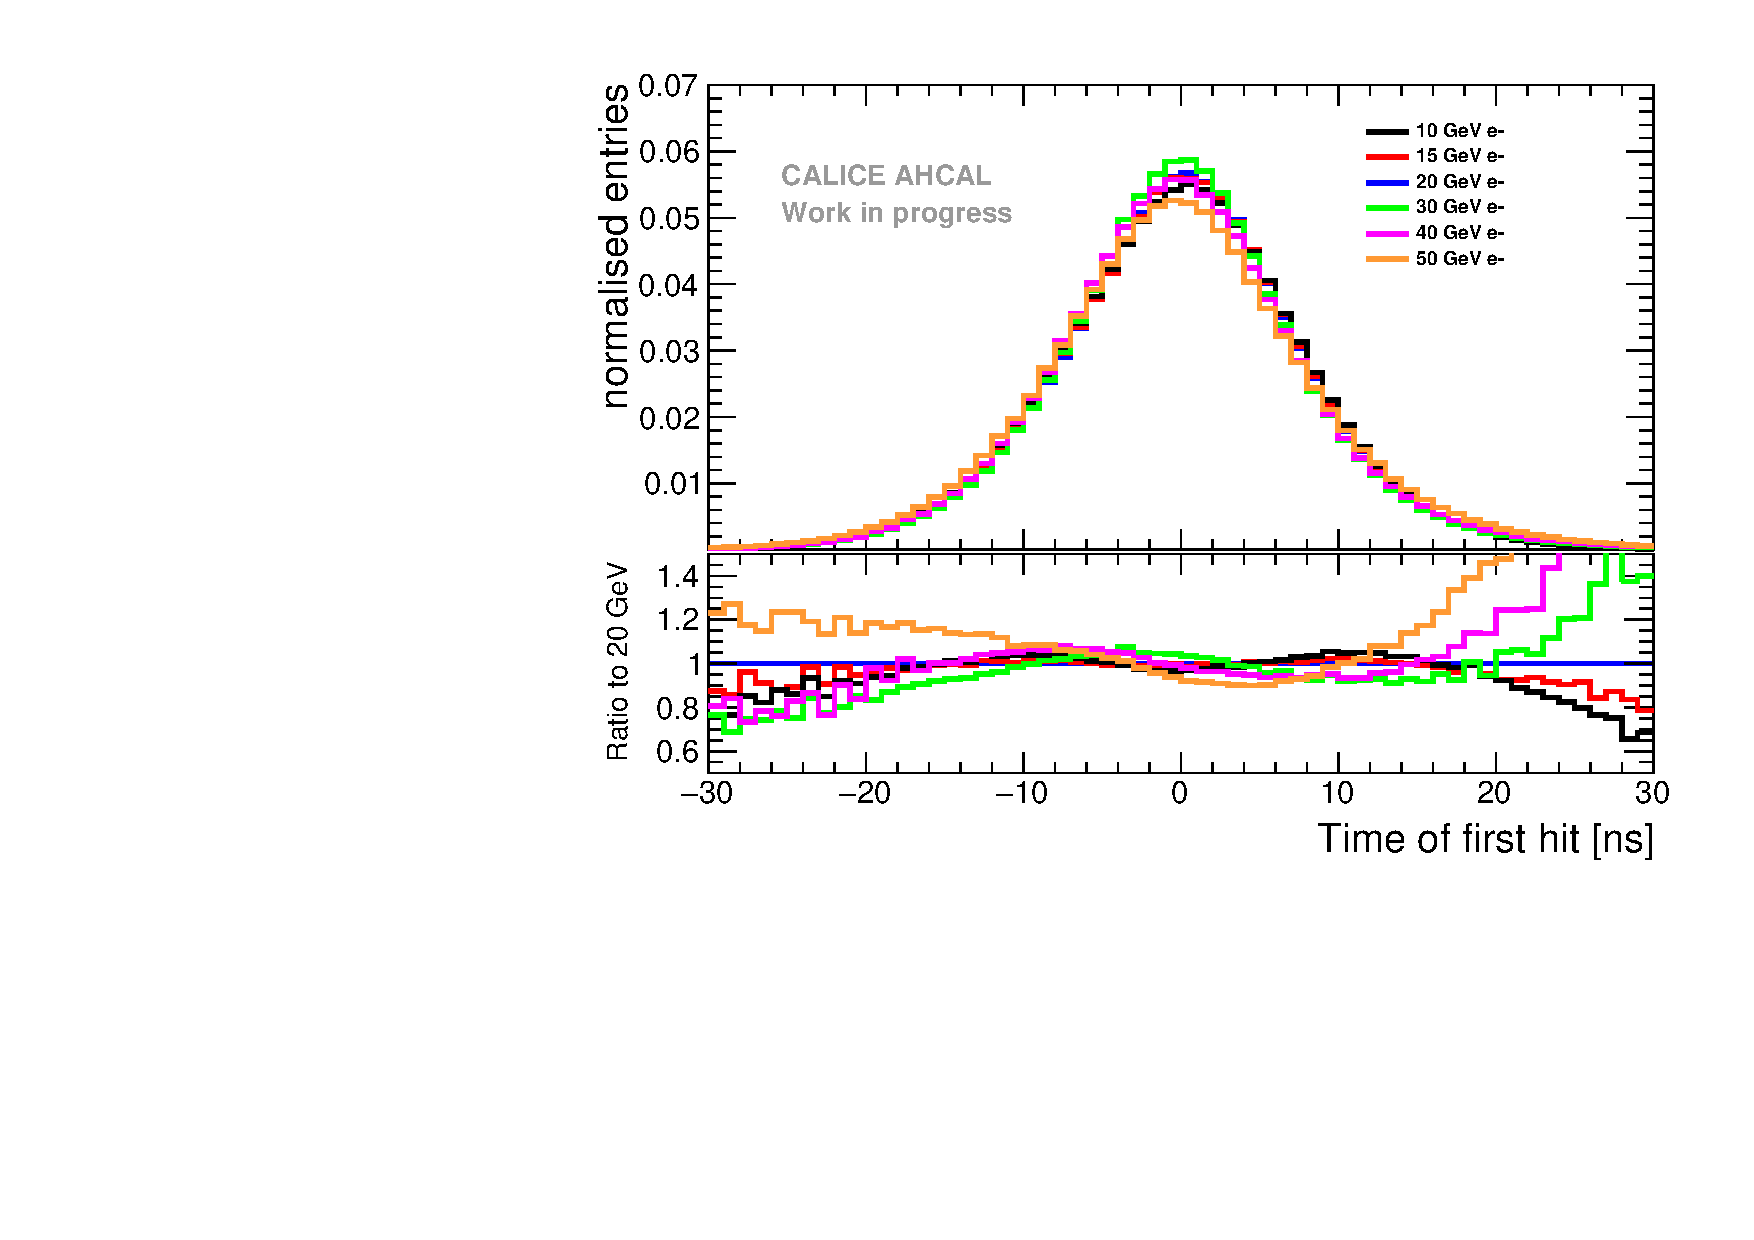
\includegraphics[width=0.6\textwidth]{chap5/fig_AHCAL_timing/Electrons/ComparisonDataEnergies.pdf}
	\caption{Comparison of the time of first hit distribution for all electron energies.}
	\label{fig:all_electron_energies}
\end{figure}

\subsection{Influence of the detector inhomogeneity}
\label{subsec:det_inhomo}

A study has been performed to estimate the influence of the detector inhomogeneity on timing independent of the beam profile. For this, only events in which the centre of gravity in x and y are within the 4 centre tiles of the detector are selected. This has been checked for 10 and 50 GeV electron beam energy. The difference between the distribution can help to estimate the systematic uncertainty due to the inhomogeneity of the detector to which electrons are very sensible to.

\begin{figure}[htbp!]
	\begin{subfigure}[t]{0.5\textwidth}
		\centering
		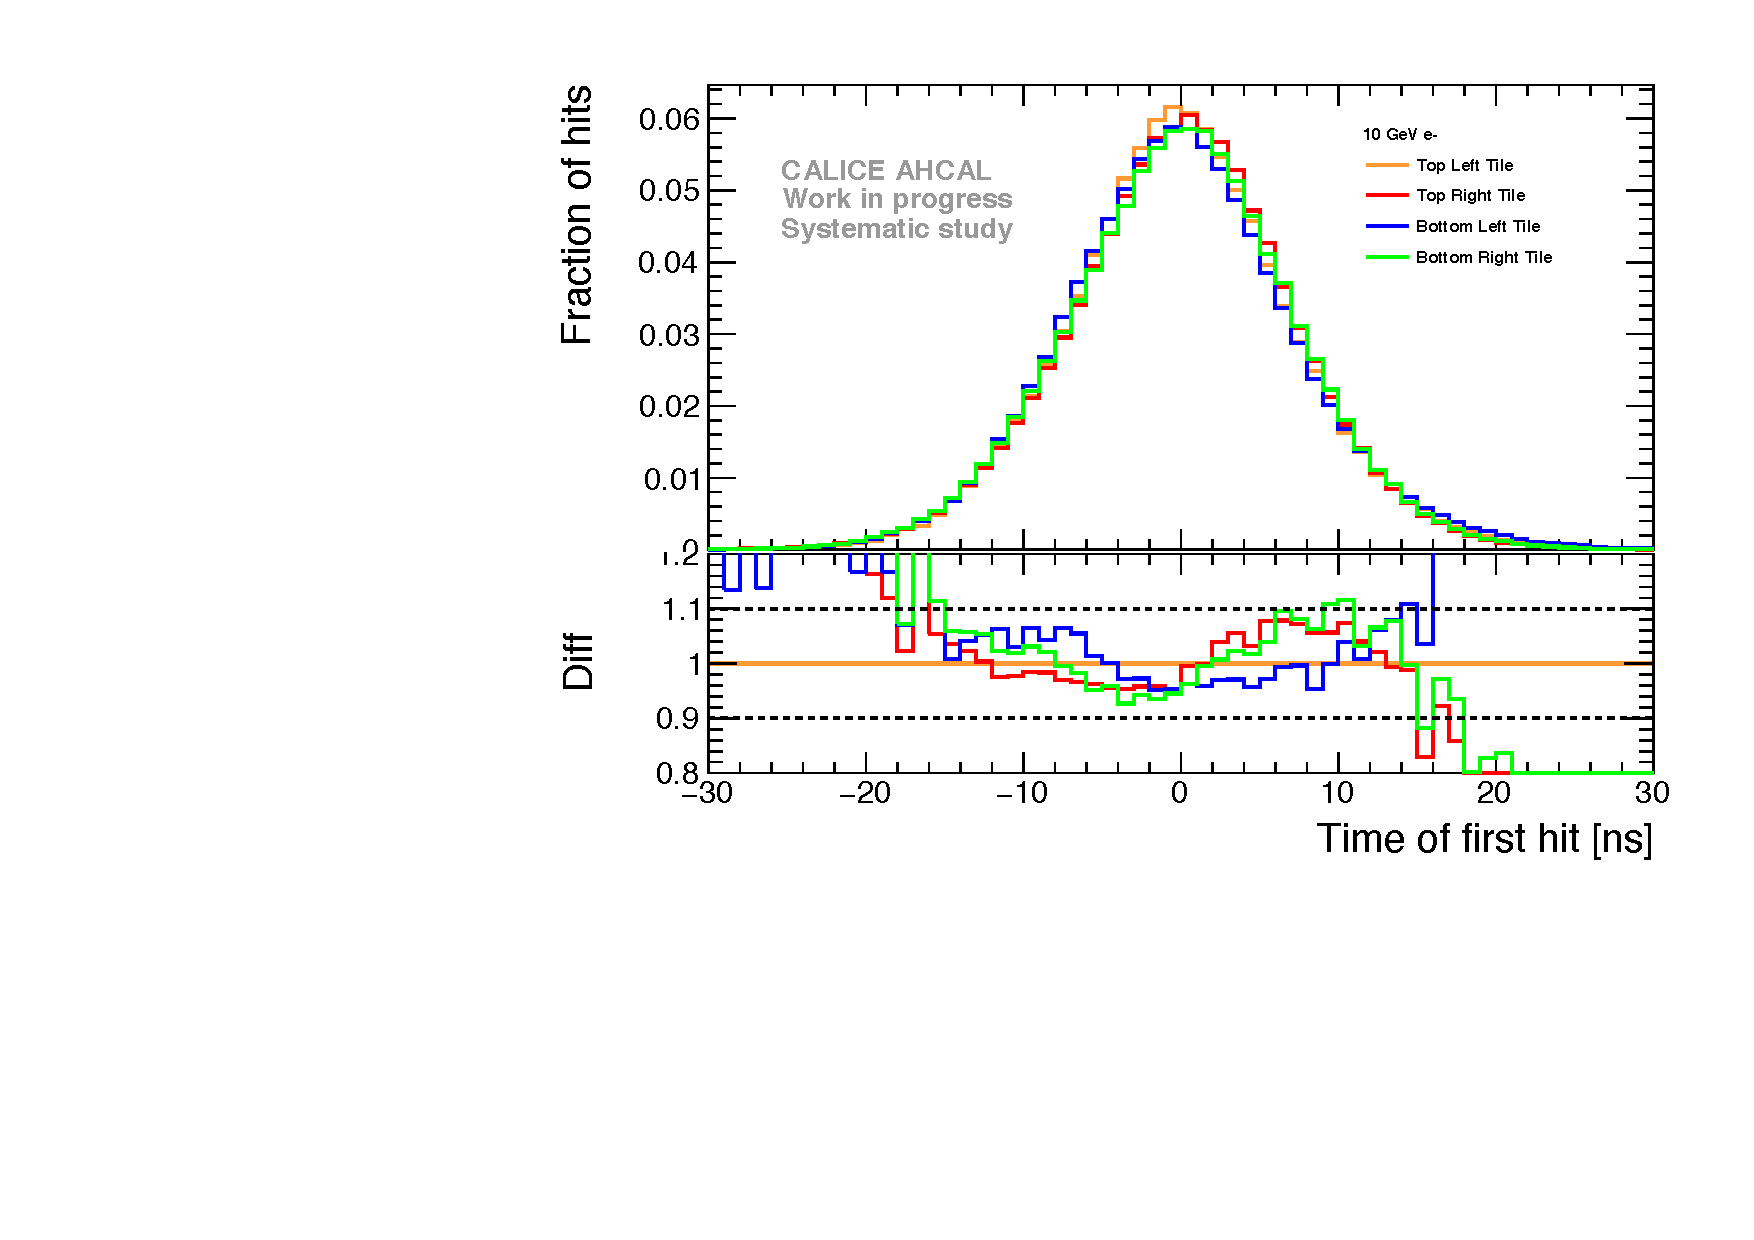
\includegraphics[width=1\textwidth]{chap5/fig_AHCAL_timing/Electrons/Systematic_Inhomogeneity_10GeV.pdf}
		\caption{Time of the first hit distribution at 10 GeV.}\label{fig:timing_inhomo_10GeV}
	\end{subfigure}
	\hfill
	\begin{subfigure}[t]{0.5\textwidth}
		\centering
		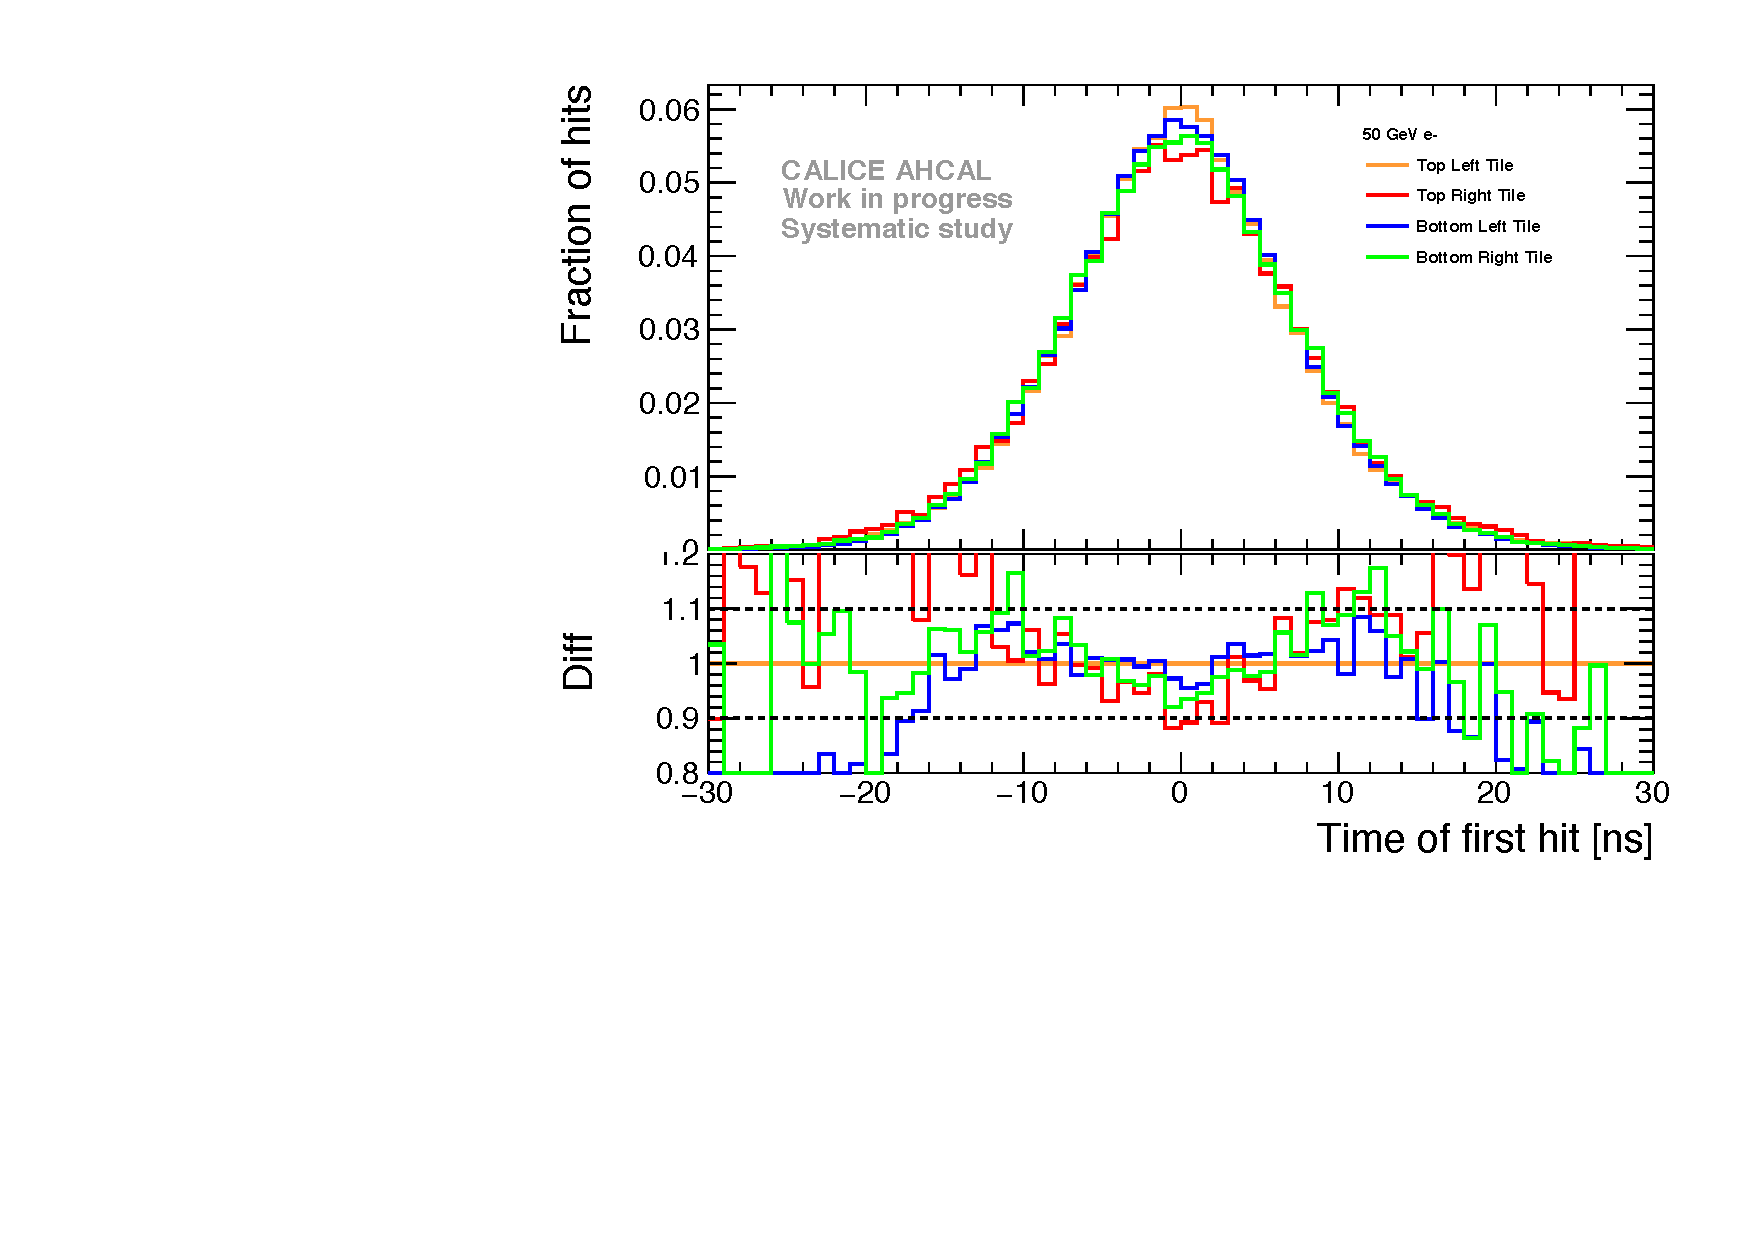
\includegraphics[width=1\textwidth]{chap5/fig_AHCAL_timing/Electrons/Systematic_Inhomogeneity_50GeV.pdf}
		\caption{Time of the first hit distribution at 50 GeV.}\label{fig:timing_inhomo_50GeV}
	\end{subfigure}
	\caption{\subref{fig:timing_inhomo_10GeV}) Time of the first hit distribution for all four middle tiles at 10 GeV. \subref{fig:timing_inhomo_50GeV}) Time of the first hit distribution for all four middle tiles at 50 GeV. All distribution are within 10-20\% in the core.}
\end{figure}

The figures \ref{fig:timing_inhomo_10GeV} and \ref{fig:timing_inhomo_50GeV} show the time distribution for each tiles at 10 and 50 GeV respectively. The ratio shown is compared to the top left centre tile. One can see that for both energies, the distributions are within a 10-20\% agreement with the region [-20, 20] ns. Therefore a conservative systematic uncertainty of 20\% is assigned to electron and pion data in the following.

\subsection{Portability of the calibration}

A small check on the transport of the calibration has been performed on another dataset from a tesbeam at DESY II in May 2016. The goal was to reuse the calibration constants obtained and apply them to another dataset in order to understand how transportable is the time calibration. The setup was composed of the same four big layers used at CERN in July 2015. In order to have enough hits in all layers, an aluminium absorber of 3 $X_{0}$ was placed in front of the detector in a 3 GeV electron beam.

\begin{figure}[htbp!]
	\centering
	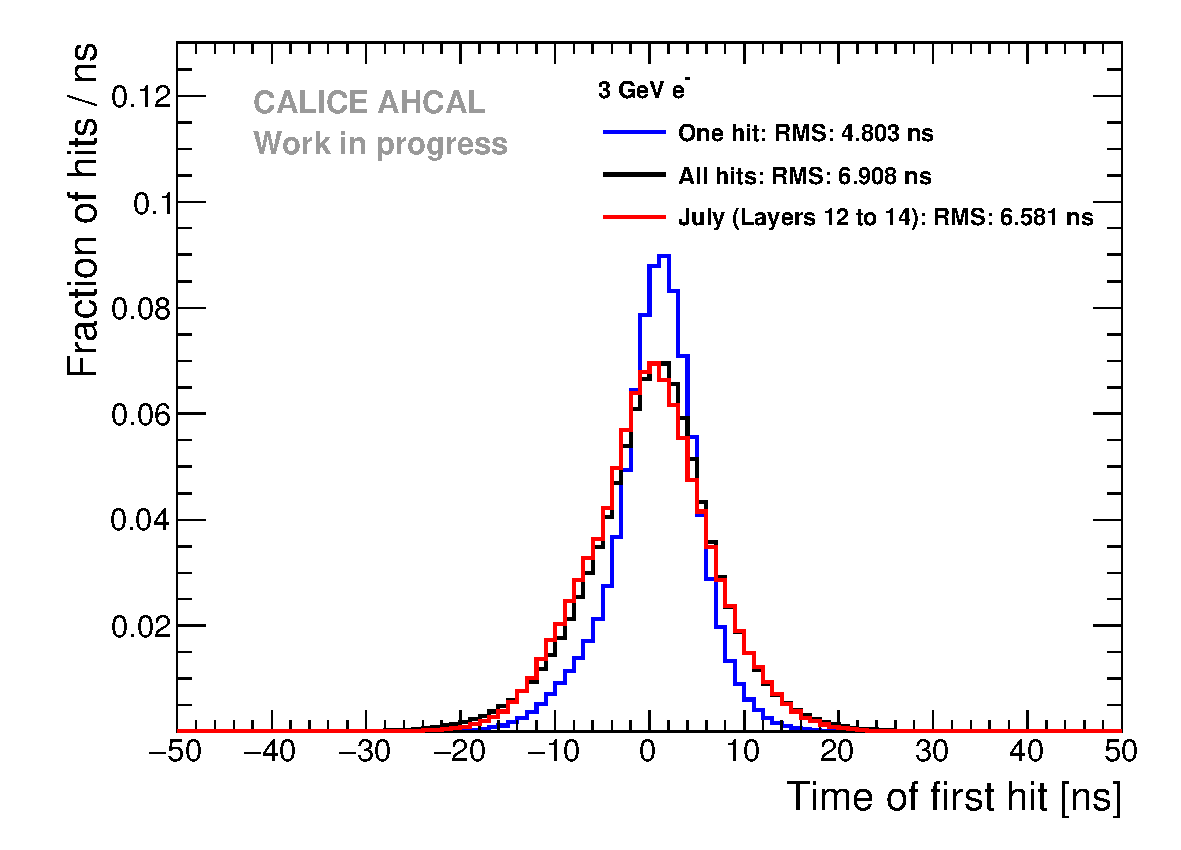
\includegraphics[width=0.5\textwidth]{chap5/fig_AHCAL_timing/Electrons/Timing_May2016_BigLayers.pdf}
	\caption{Time of the first hit distribution for 3 GeV electron showers at the DESY II testbeam in May 2016.}\label{fig:TBMay2016}
\end{figure}

The same calibration constants were used except a small re-calibration of the trigger channels ($T_{0}$) was performed. The figure \ref{fig:TBMay2016} shows the distribution of the time of first hits for layer 13 and 14. The time resolution obtained of 7 ns is somewhat very close to the time resolution obtained in July 2015. The difference may come from the fact that different layers were used in the testbeam at CERN compared to DESY. Despite this, it gives a good hint that the calibration constants are to some extent transportable to a different testbeam configuration.

\section{Validation of the simulation}

\begin{table}[htb!]
	\centering
	\caption{Timing resolution extracted with a double Gaussian fit from muon data used for simulation.}
	\label{table:time_res_sim}
	\begin{tabular}{@{} cccccc @{}}
		\hline
		$\alpha_{1}$ & $\mu_{1}$ [ns] & $\sigma_{1}$ [ns] & $\alpha_{2}$ & $\mu_{2}$ [ns] & $\sigma_{2}$ [ns] \\
		\hline
		0.607352 & -0.699093 & 5.85891 & 0.391041 & 0.945272 & 3.4012 \\
		\hline
	\end{tabular}
\end{table}

The next step is to compare data with simulation. The timing resolution is extracted from muon data runs by fitting a double Gaussian to the data in the range [-50 ns, 50 ns] and is used to smear the timing of simulated calorimeter hits. The table \ref{table:time_res_sim} sums up the parameters used. The comparison for muons is shown in figure \ref{fig:sim_data_muon}. The comparison shows that in the full range, the difference between data and simulation is around 10-20\% maximum. In general, the simulation is in a good agreement with data.

\begin{figure}[htbp!]
	\centering
	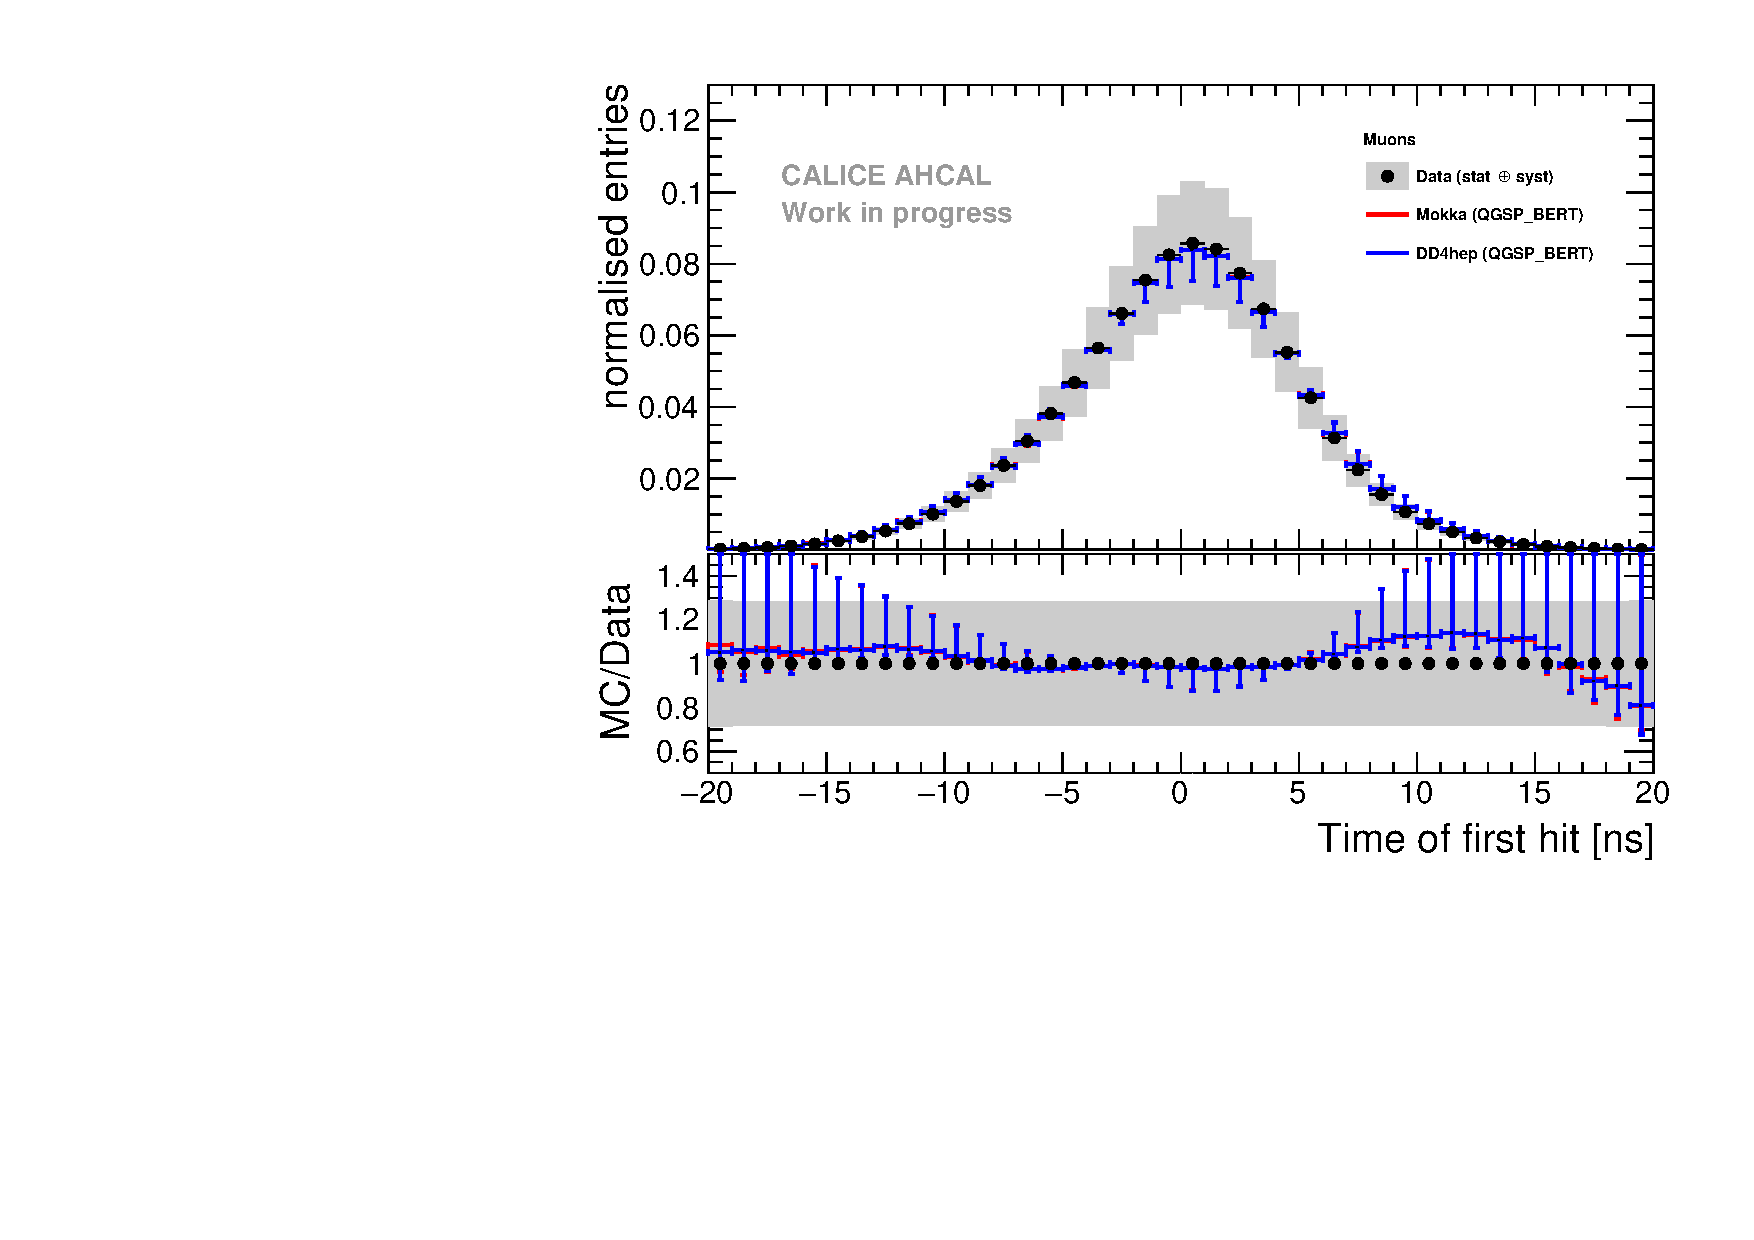
\includegraphics[width=0.6\textwidth]{chap5/fig_AHCAL_timing/Muons/Comparison_MokkaDD4hepData_Muons.pdf}
	\caption{Time of first hit for data and simulation between -20 and 20 ns.}
	\label{fig:sim_data_muon}
\end{figure}

In the next step, a comparison with electron data is necessary to validate the simulation. In addition to the muon resolution, a parametrisation of the increase of the width of the time distribution function of the number of hits above 0.5 MIPs is added in simulation as described in appendix \ref{appendix:ped_shift}. The figures \ref{fig:sim_data_elec} shows this comparison.

\begin{figure}[htbp!]
	\begin{subfigure}[t]{0.5\textwidth}
		\centering
		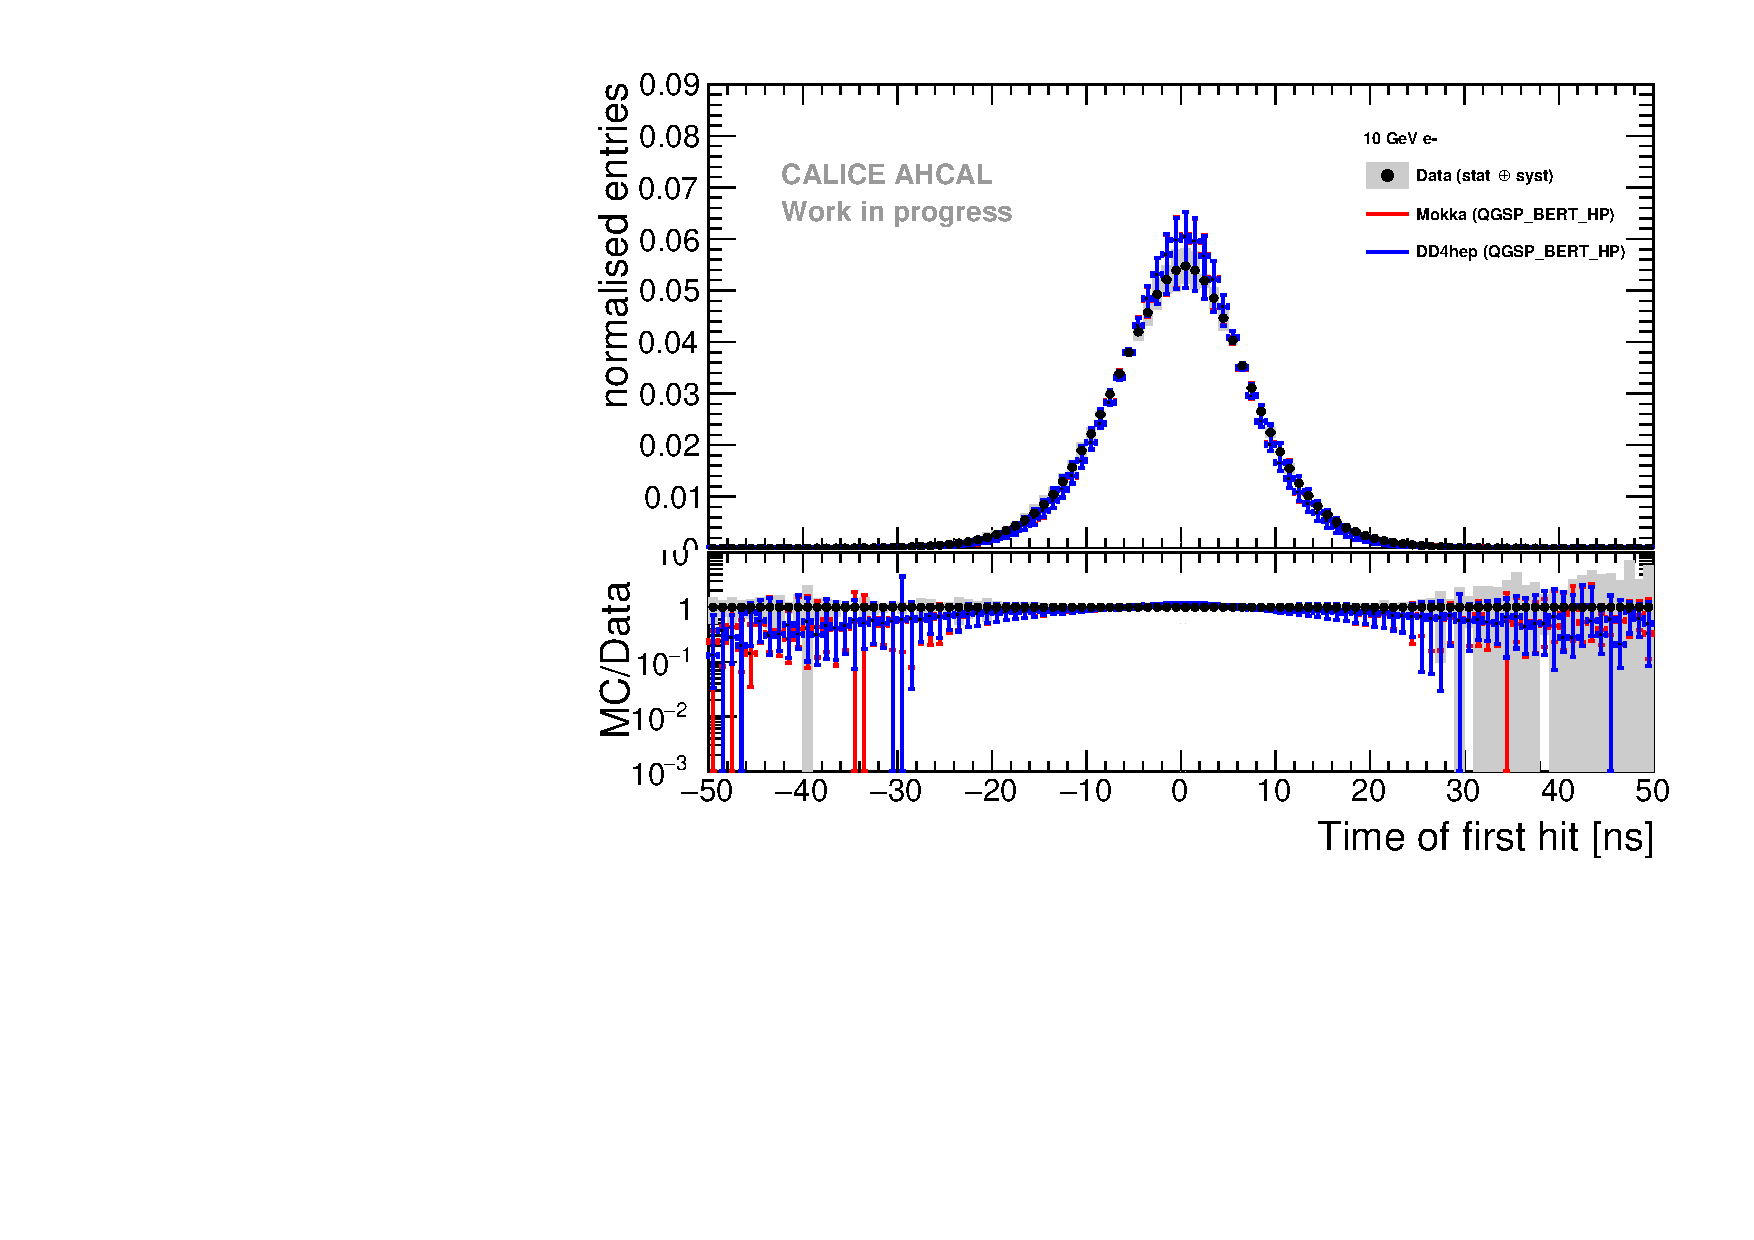
\includegraphics[width=1\textwidth]{chap5/fig_AHCAL_timing/Electrons/Comparison_SimData_Electrons10GeV.pdf}
		\caption{10 GeV.}\label{fig:elec_sim_data_10GeV}
	\end{subfigure}
	\hfill
	\begin{subfigure}[t]{0.5\textwidth}
		\centering
		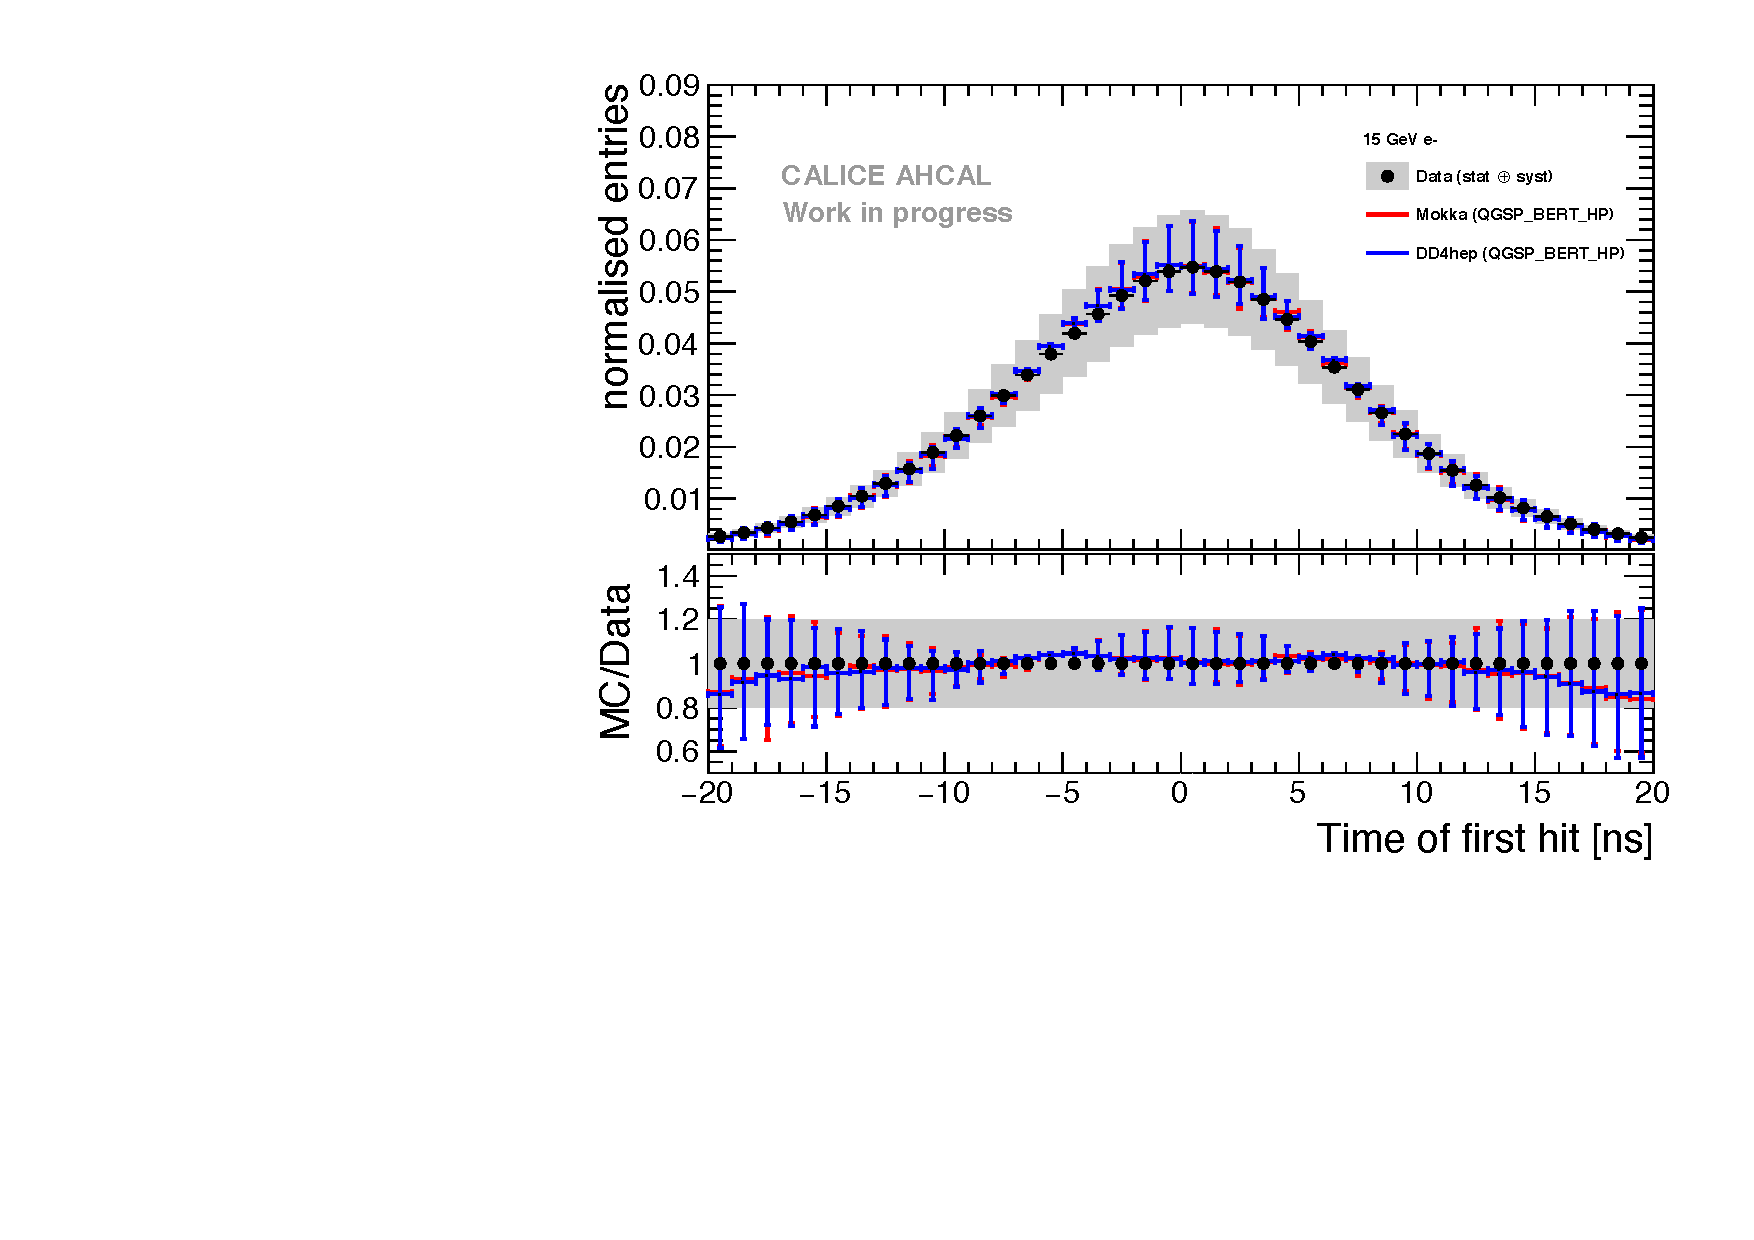
\includegraphics[width=1\textwidth]{chap5/fig_AHCAL_timing/Electrons/Comparison_SimData_Electrons15GeV.pdf}
		\caption{15 GeV.}\label{fig:elec_sim_data_15GeV}
	\end{subfigure}
	\hfill
	\begin{subfigure}[t]{0.5\textwidth}
		\centering
		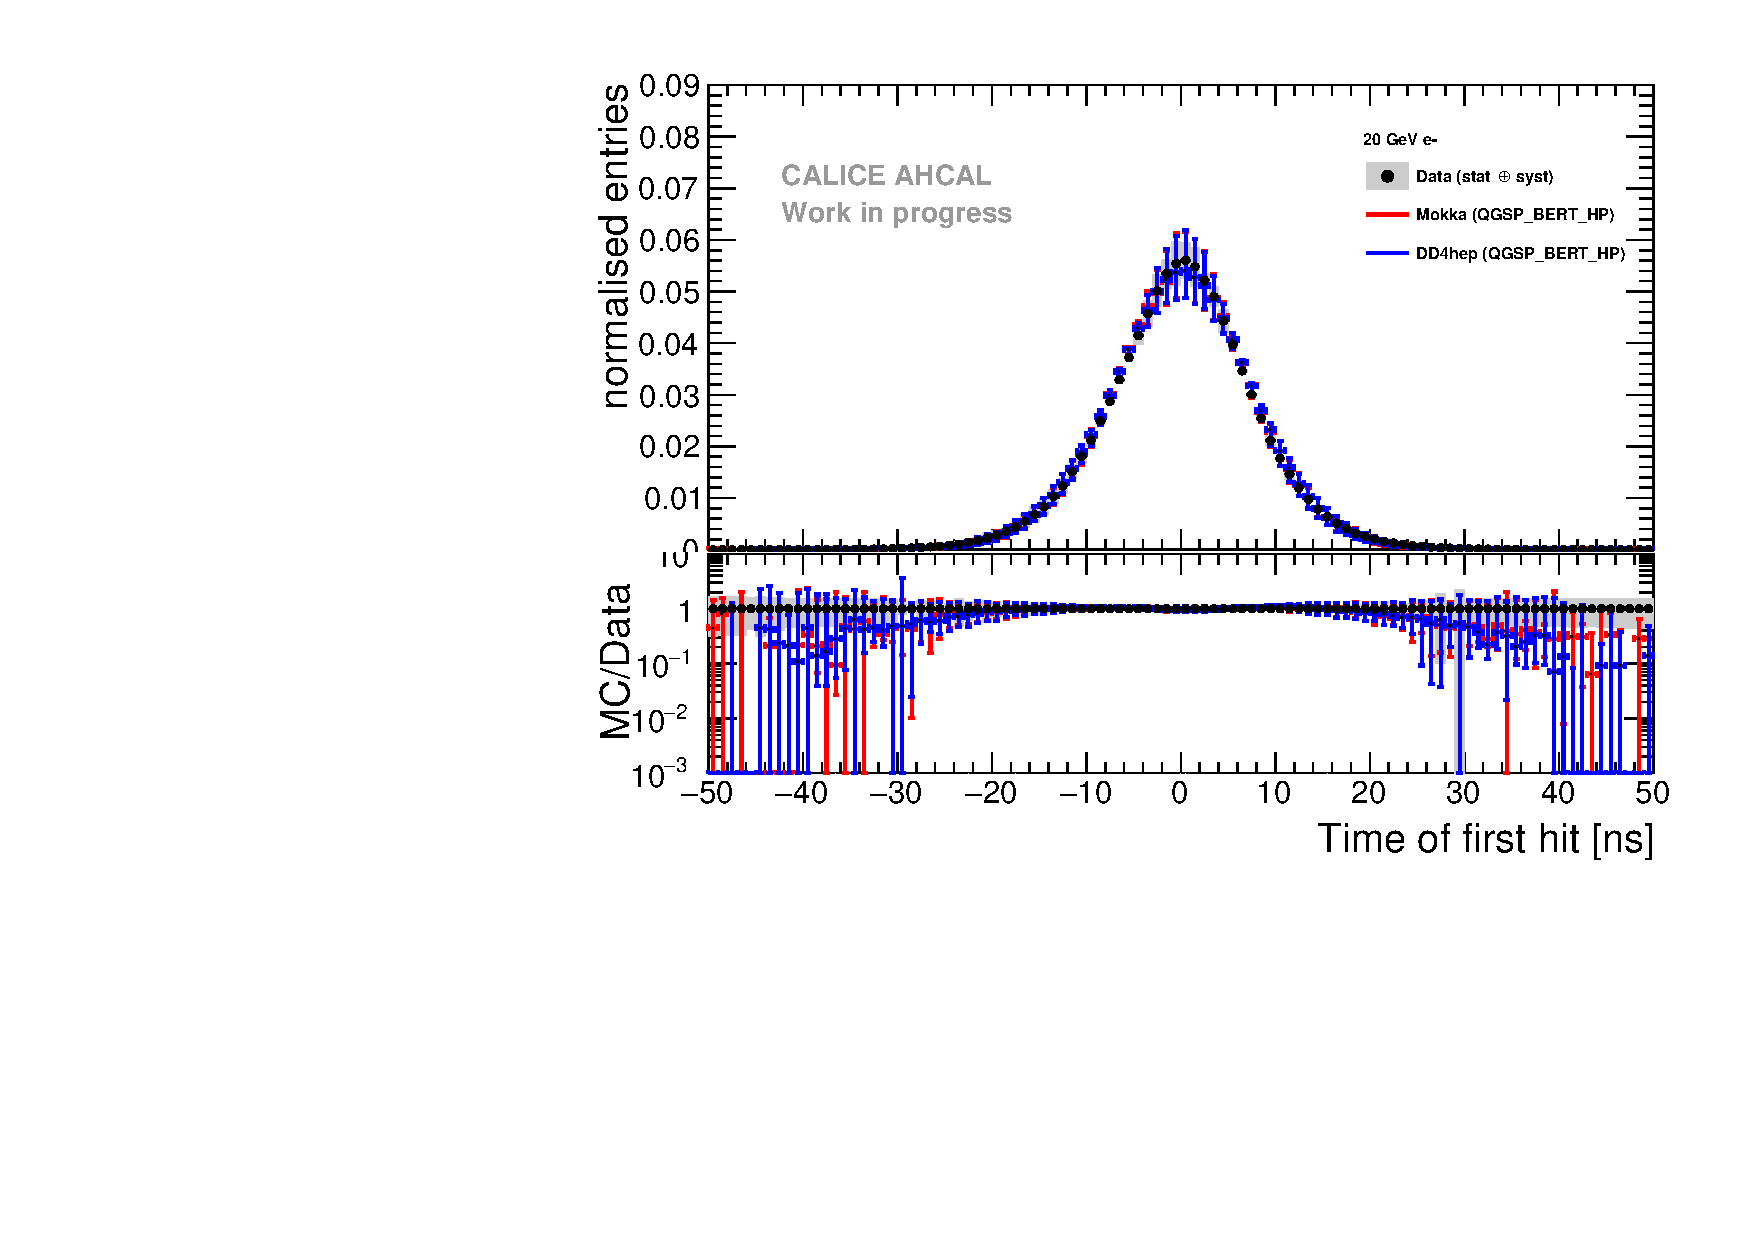
\includegraphics[width=1\textwidth]{chap5/fig_AHCAL_timing/Electrons/Comparison_SimData_Electrons20GeV.pdf}
		\caption{20 GeV.}\label{fig:elec_sim_data_20GeV}
	\end{subfigure}
	\hfill
	\begin{subfigure}[t]{0.5\textwidth}
		\centering
		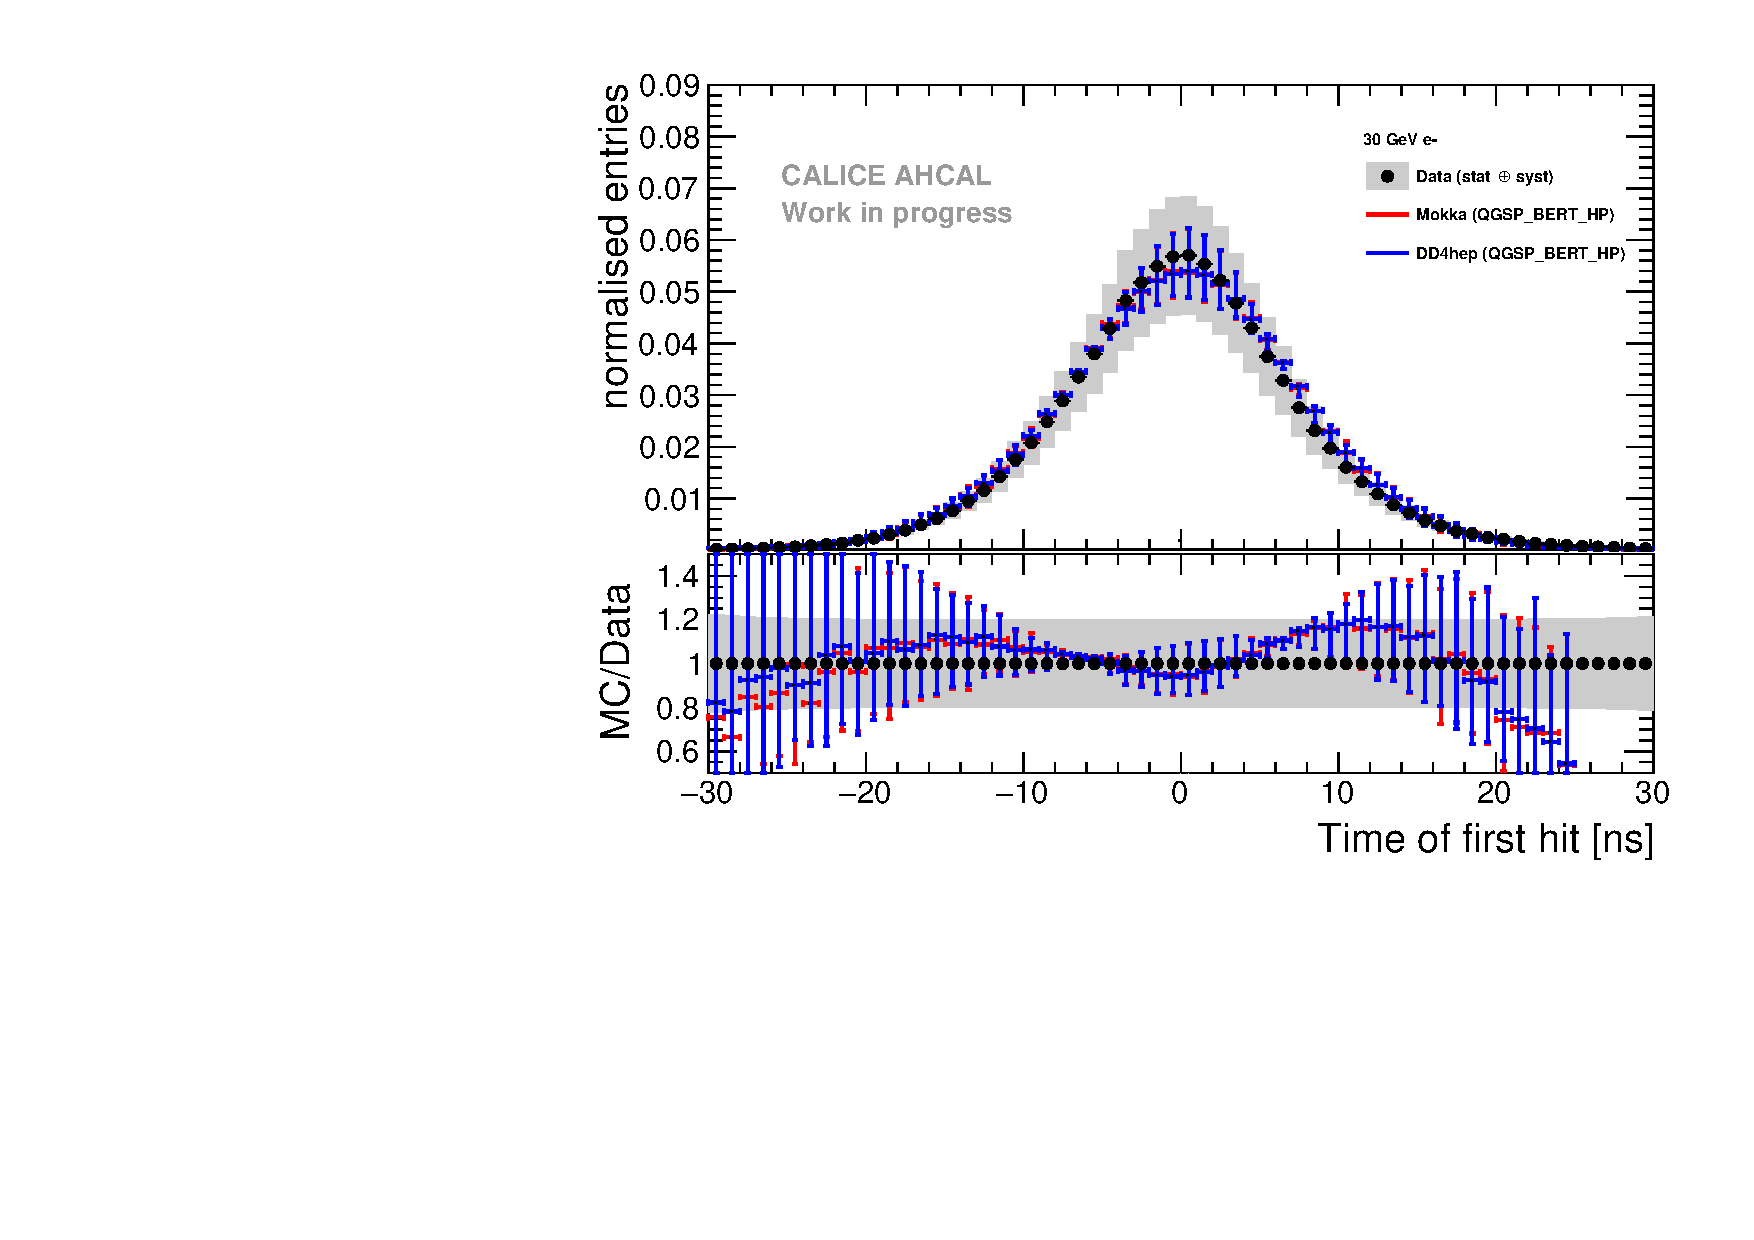
\includegraphics[width=1\textwidth]{chap5/fig_AHCAL_timing/Electrons/Comparison_SimData_Electrons30GeV.pdf}
		\caption{30 GeV.}\label{fig:elec_sim_data_30GeV}
	\end{subfigure}
	\hfill
	\begin{subfigure}[t]{0.5\textwidth}
		\centering
		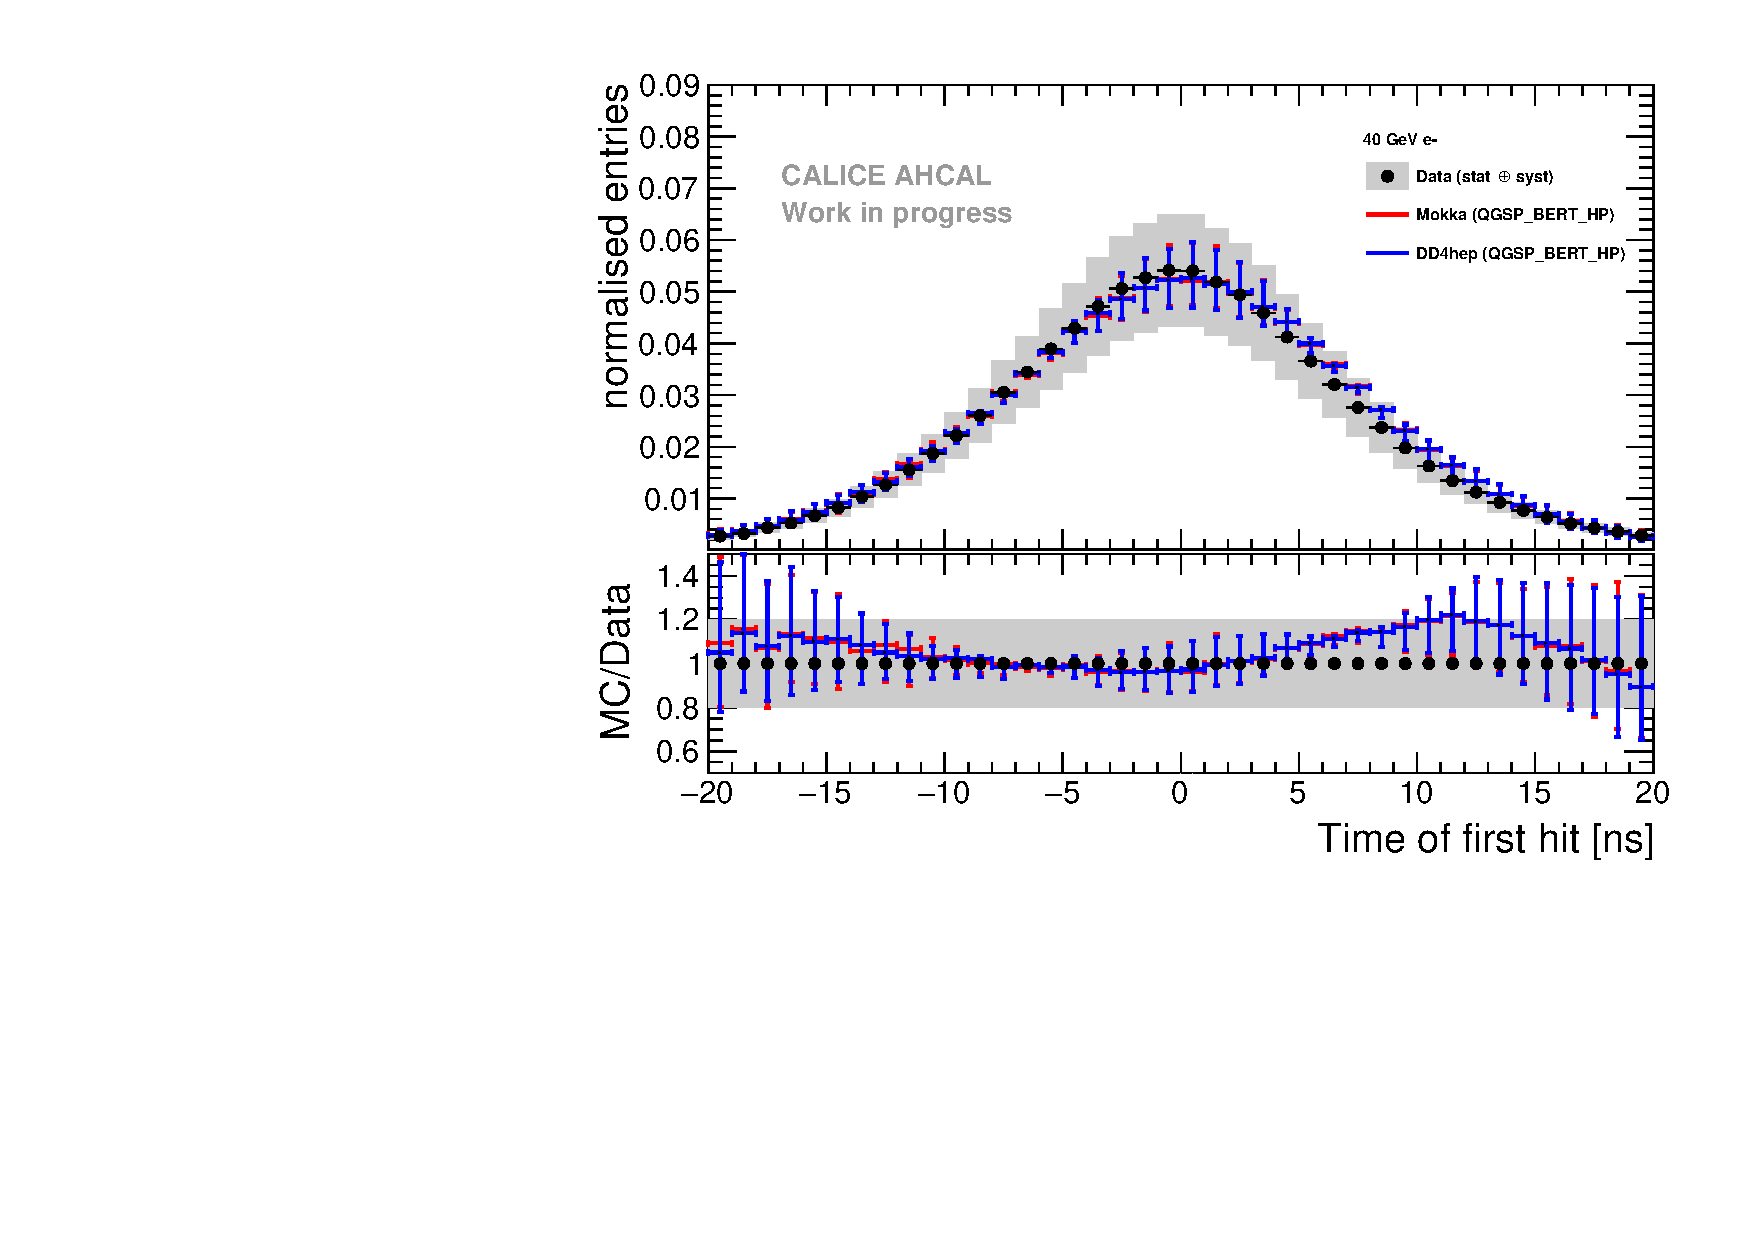
\includegraphics[width=1\textwidth]{chap5/fig_AHCAL_timing/Electrons/Comparison_SimData_Electrons40GeV.pdf}
		\caption{40 GeV.}\label{fig:elec_sim_data_40GeV}
	\end{subfigure}
	\hfill
	\begin{subfigure}[t]{0.5\textwidth}
		\centering
		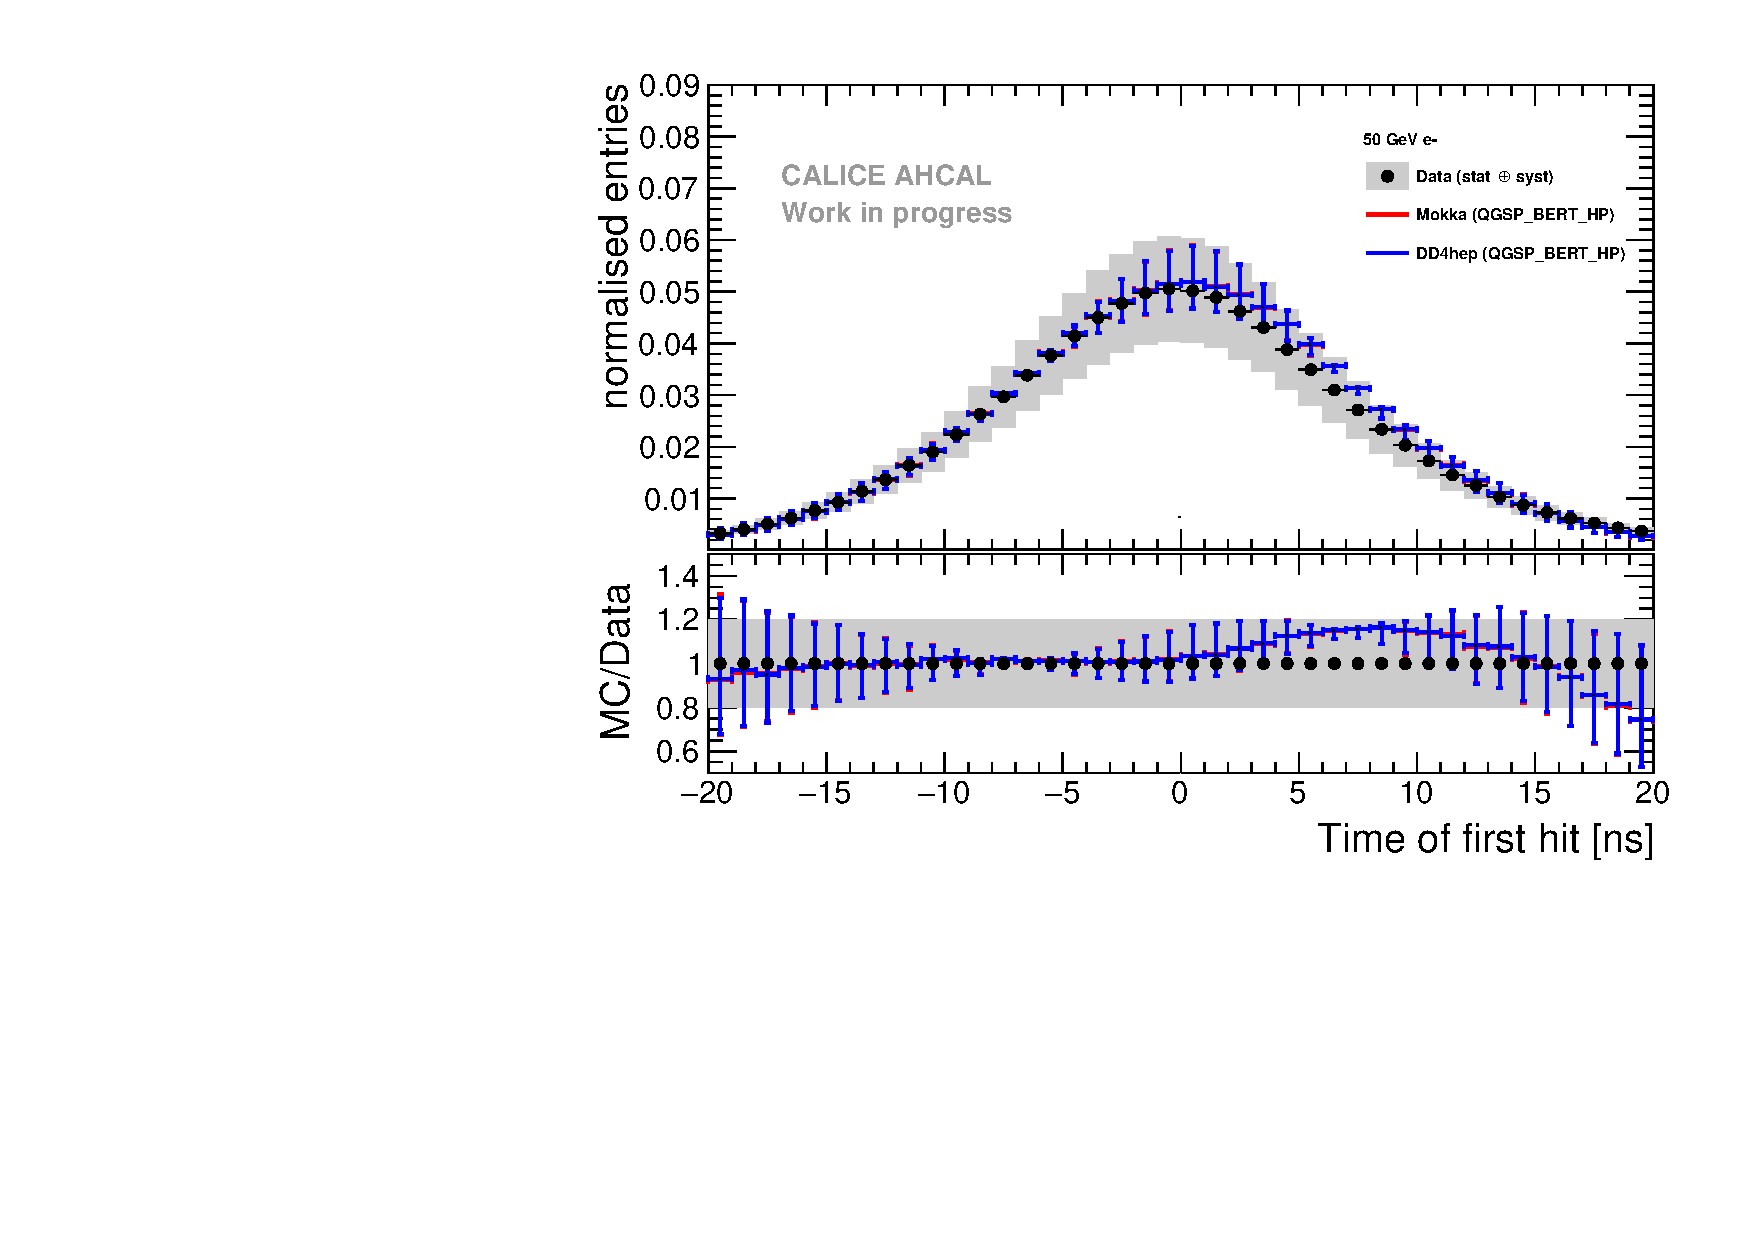
\includegraphics[width=1\textwidth]{chap5/fig_AHCAL_timing/Electrons/Comparison_SimData_Electrons50GeV.pdf}
		\caption{50 GeV.}\label{fig:elec_sim_data_50GeV}
	\end{subfigure}
	\caption{Comparison between electron data and MC for all energies of the time of first hit. The grey area represents the statistical and systematical error of the data. Error bars in simulation are obtained by varying the cross-talk parameter and with the error envelope from the number of hits parameterisation.}
	\label{fig:sim_data_elec}
\end{figure}

The simulation is systematically narrower than data for all energies. This would suggest that simulation has less hits than data which is in agreement with figures \ref{fig:sim_data_elec_nHits}, where generally simulation is 10-20\% lower than data in the region of interest of 6 to 10 hits per chip. The simulation is in better agreement for higher energies, at 40-50 GeV, than for lower energies at 10-15 GeV. This may come from imperfect beam profiles where a slight shift in simulation can influence highly the number of triggers in a chip. As well the parametrisation may be imperfect and may suggest that the time parametrisation could be chip-wise or layer-wise. But due to the limited amount of data, only a global time parametrisation can be applied. For 10 to 20 GeV comparisons, the description of the tails in simulation are quite underestimated. This may be due to the description of the noise in simulation that is not perfectly reproduced. Overall, the simulation and data are in agreement within statistical and systematic uncertainties.

\begin{figure}[htbp!]
	\begin{subfigure}[t]{0.5\textwidth}
		\centering
		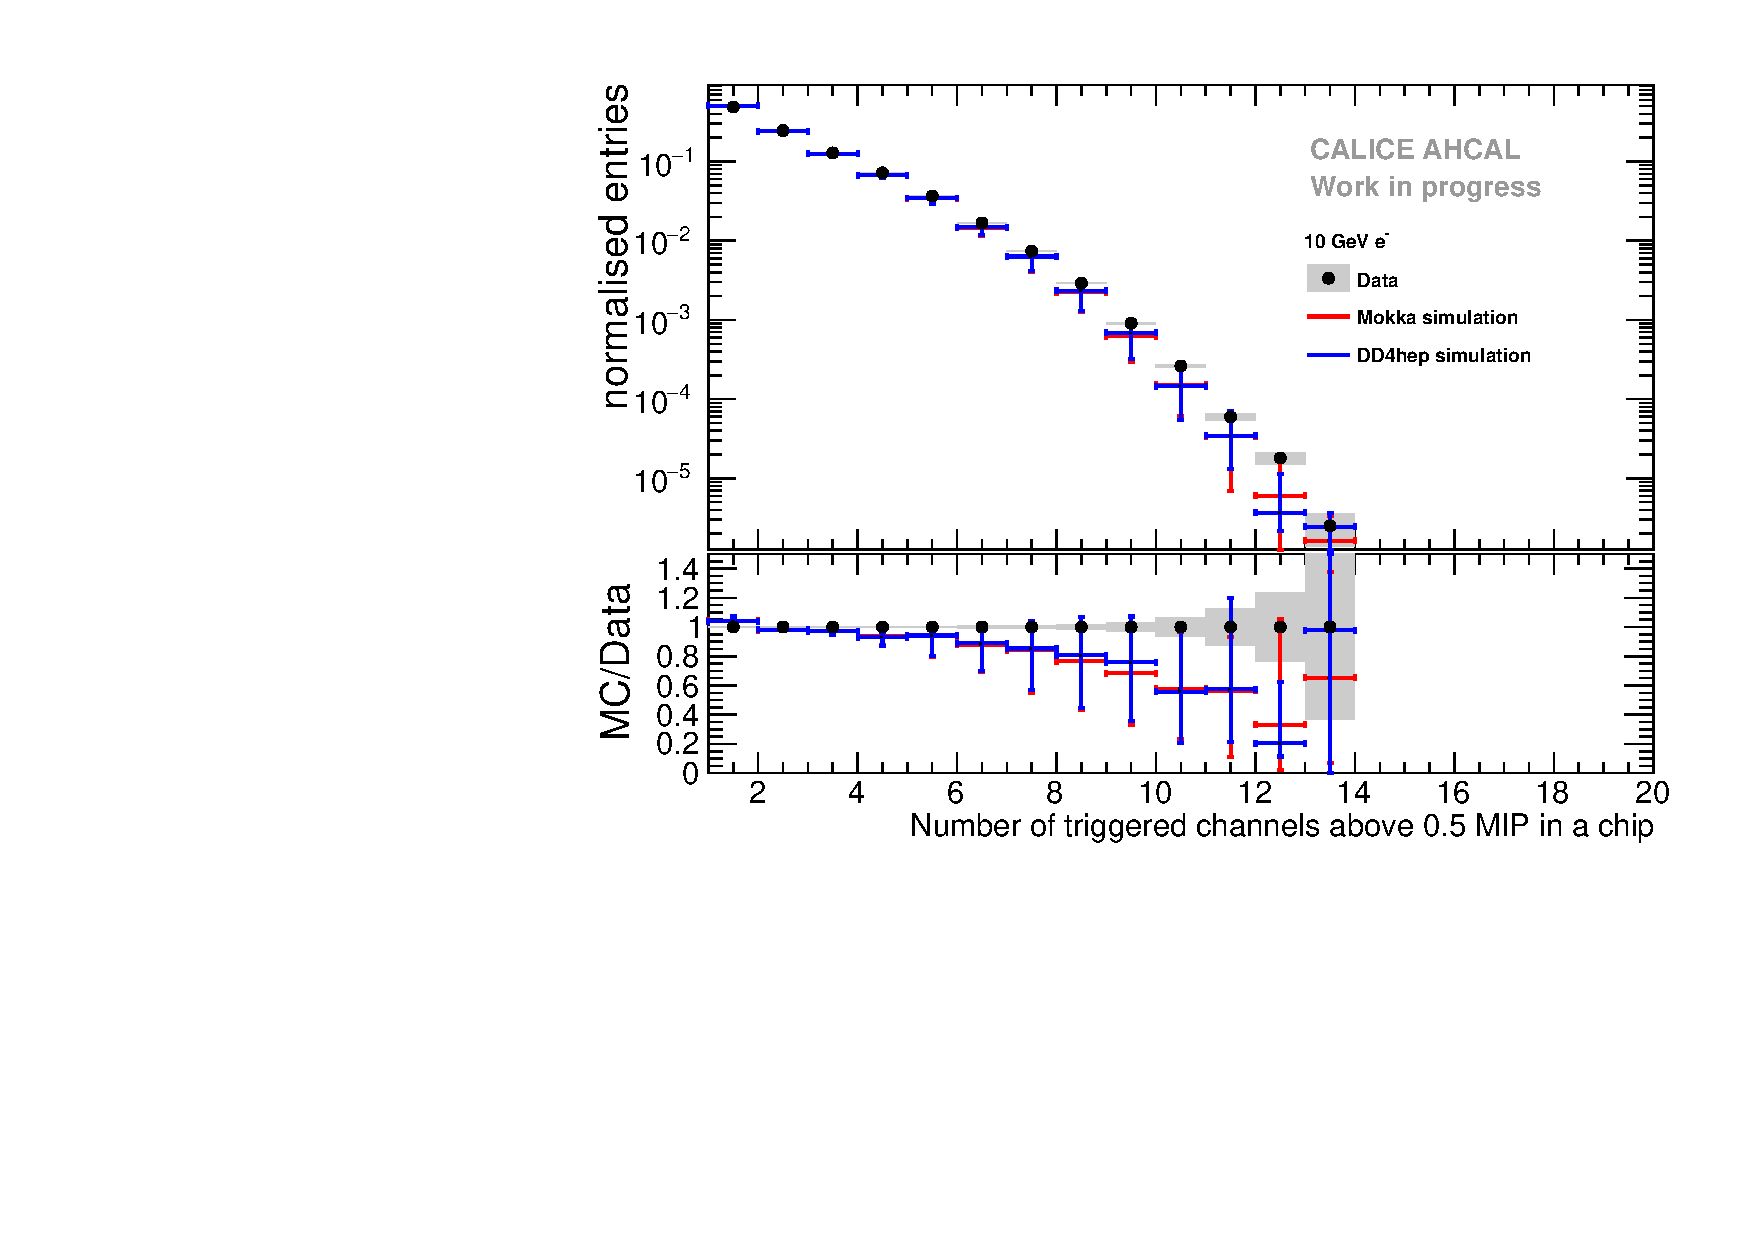
\includegraphics[width=1\textwidth]{chap5/fig_AHCAL_timing/Electrons/Comparison_SimData_Electrons_nHits_10GeV.pdf}
		\caption{10 GeV.}\label{fig:elec_sim_data_nHits_10GeV}
	\end{subfigure}
	\hfill
	\begin{subfigure}[t]{0.5\textwidth}
		\centering
		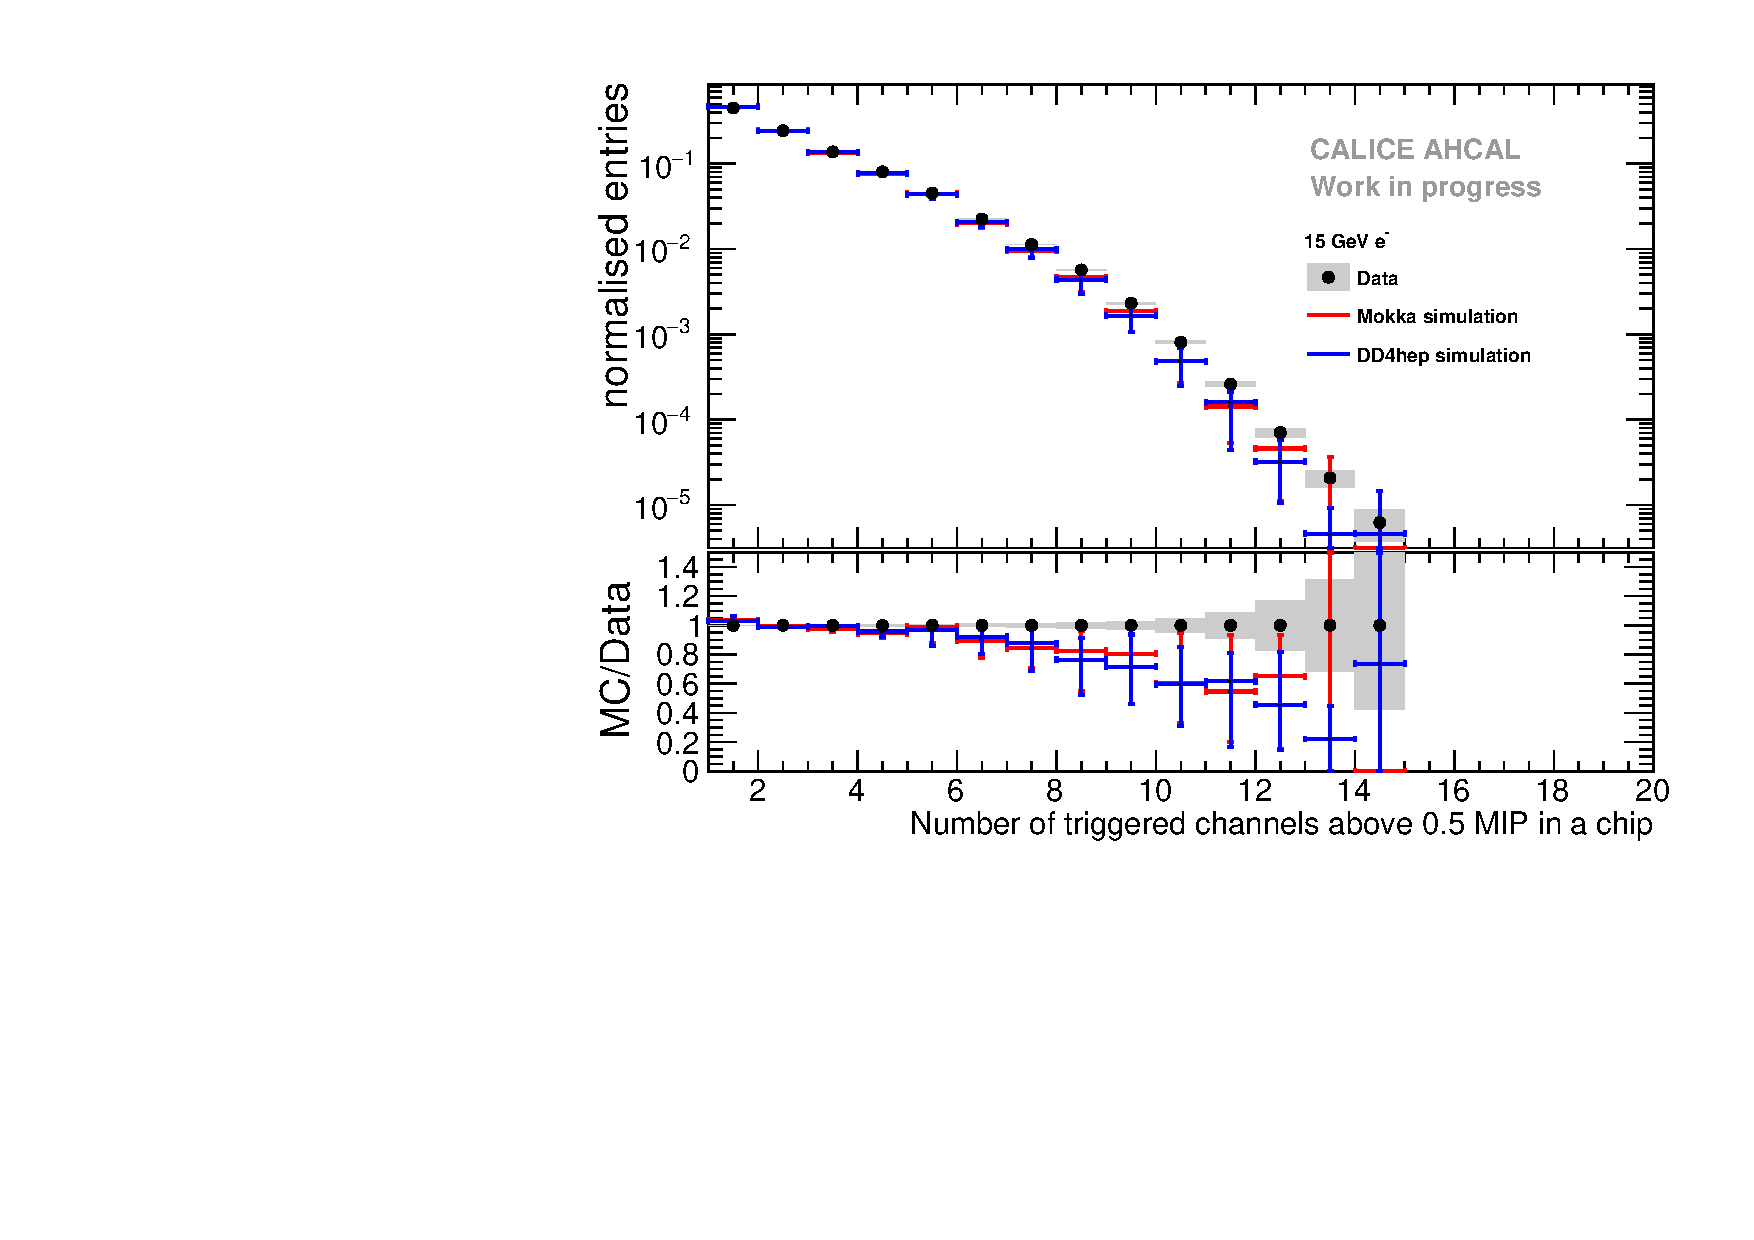
\includegraphics[width=1\textwidth]{chap5/fig_AHCAL_timing/Electrons/Comparison_SimData_Electrons_nHits_15GeV.pdf}
		\caption{15 GeV.}\label{fig:elec_sim_data_nHits_15GeV}
	\end{subfigure}
	\hfill
	\begin{subfigure}[t]{0.5\textwidth}
		\centering
		\includegraphics[width=1\textwidth]{chap5/fig_AHCAL_timing/Electrons/Comparison_SimData_Electrons_nHits_20GeV.pdf}
		\caption{20 GeV.}\label{fig:elec_sim_data_nHits_20GeV}
	\end{subfigure}
	\hfill
	\begin{subfigure}[t]{0.5\textwidth}
		\centering
		\includegraphics[width=1\textwidth]{chap5/fig_AHCAL_timing/Electrons/Comparison_SimData_Electrons_nHits_30GeV.pdf}
		\caption{30 GeV.}\label{fig:elec_sim_data_nHits_30GeV}
	\end{subfigure}
	\hfill
	\begin{subfigure}[t]{0.5\textwidth}
		\centering
		\includegraphics[width=1\textwidth]{chap5/fig_AHCAL_timing/Electrons/Comparison_SimData_Electrons_nHits_40GeV.pdf}
		\caption{40 GeV.}\label{fig:elec_sim_data_nHits_40GeV}
	\end{subfigure}
	\hfill
	\begin{subfigure}[t]{0.5\textwidth}
		\centering
		\includegraphics[width=1\textwidth]{chap5/fig_AHCAL_timing/Electrons/Comparison_SimData_Electrons_nHits_50GeV.pdf}
		\caption{50 GeV.}\label{fig:elec_sim_data_nHits_50GeV}
	\end{subfigure}
	\caption{Comparison between electron data and MC for all energies of the number of triggered channels per chip. The grey area represents the statistical error of the data. Error bars in simulation are obtained by varying the cross-talk parameter between 10\% and 18\%.}
	\label{fig:sim_data_elec_nHits}
\end{figure}

\section{Timing of the pion data}

The table \ref{table:pion_runs} summarises the runs and datasets used for the pion analysis. The calibration is applied to pion data directly after the selection. The pion selection is applied and the same trigger reference selection is use to select events. The table shows that more 80\% of the events pass the trigger selection.

{
\renewcommand{\arraystretch}{1.5}
\begin{table}[htb!]
	\centering
	\caption{Table with the statistic before and after selection used for the pion dataset.}
	\label{table:pion_runs}
	%\resizebox{0.9\textwidth}{!}{%
	\begin{tabularx}{\textwidth}{>{\hsize=1.1\hsize}Xlllll}
		\hline
		Runs & Energy & Particle Type & Events (3 T0s) & Events (sel.) & $\frac{\text{N$_{sel.}$}}{\text{N$_{raw}$}}$ \\
		\hline
		24306-24317 \newline 24381-24397 & 10 GeV & $\pi^-$ & 425517 & 349012 & 82\% \\
		\hline
		24578-24612 & 50 GeV & $\pi^-$ & 1183790 & 1007889 & 85.1\% \\
		\hline
		24339-24342 & 70 GeV & $\pi^-$ & 142813 & 122376 & 85.7\% \\
		\hline
		24223-24238 \newline 24273-24287 \newline 24331-24336 \newline 24358-24364 & 90 GeV & $\pi^-$ & 466927 & 395884 & 84.8\% \\
		\hline
	\end{tabularx}
	%}
\end{table}
}

\subsection{Systematic uncertainties}

For a significant assesment of differences observed between data and simulations, systematic errors must be evaluated. Several possible errors where identified:

\begin{itemize}
	% \item MIP Energy Scale: An error on the MIP energy scale needs to be converted in time when looking at the dependence of time with hit energy. An error of 0.5\% is taken. Using simulation, this can be converted into time. For muon and electron beams, it has mostly no effects. For pion beams, it ranges from XXX ns at 0.5 MIP to XXX ns at 1 MIP.
	\item Non-Linearity correction: A non-linearity correction is applied to the data as explained in section \ref{subsec:lin_corr}. The residuals of the correction give a systematic error at the level of 0.2 ns.
	\item Time walk correction: In the same way as for the non-linearity correction, the error obtained from the residuals of the correction is in the order of 0.2 ns.
	\item Number of triggered channels correction: the correction for the number of triggered channels over 0.5 MIP in a chip results in a residual on the timing in the order of 1 ns. This systematic error is the most dominant over all other uncertainties.
	\item Determination of the offset to $t=0$: A shift of the time distribution at zero is done for each layer. The error of this shift varies between 0.05 to 0.1 ns for data. In this case, a conservative error of 0.1 ns is used. For simulation, the shift can be calculated easily using a simple time of flight correction $T_{of} = \frac{z_{layer}}{c}$ with $c$ the speed of light and $z_{layer}$ the z position of a layer. For this a uncertainty of 3 mm is taken in z corresponding to 0.01 ns error in timing.
	\item Position relative of the detector to the beam: The detector was positionned in a way that the beam hits mostly the centered tiles. The uncertainty of the position of the layers is at the centimeter level. Thus a conservative error of a tile (3 cm) is taken. This uncertainty converted to time using QGSP\_BERT\_HP varies between 0.36 ns at $r = 1.5$ cm to 1.27 ns at $r = 19.5$ cm for the small layers and between 0.15 ns at $r = 1.5$ cm to 0.67 ns at $r = 31.5$ cm for the big layers using 10 GeV data. For each beam energy, the systematics were determined.
	\item Cross-talk: No measurement for cross-talk is available and from previous measurements it varies between 10\% and 18\%. These are used for systematics in simulation.
	\item Detector inhomogeneities: Following a small study of timing independant of the beam profile, variations in the absolute number of entries in each time bins can be observed. The variations are between 10-20\% thus a conservative error of 20\% is used for the time distribution.
	\item Number of events: In the pion data, some possible contamination from multi-particle events may be present still after the selection. Thus the number of absolute pion events is not known. A conservative error of 10\% when comparing data to simulation for the absolute number of hits per time bin.
	\item Smearing parametrisation: A parametrisation was obtained from data for the width of the time smearing as function of the number of triggered channels. An error band was obtained by comparing all electron energies as explained in appendix \ref{appendix:ped_shift}. This is applied to simulation for systematics.
\end{itemize}

The systematics errors are added in quadrature for the full systematic. For comparison data-MC of the number of hits per time bin, an error of 20\% for muons/electrons and 30\% for pions is used. For the distribution of time versus energy, the systematic error is resulting at 1.04 ns. For the distribution of time versus radius, the systematic error is varying between 0.36 ns at small radius to 1.54 ns at large radius for the small layers and from 0.15 ns at small radius to 0.95 ns at large radius for the big layers. The table \ref{table:time_syst} sums up the systematic errors used in the analysis.
%% Systematics from number of hits may be underestmated... %
{
\renewcommand{\arraystretch}{1.2}
\begin{table}[htb!]
	\centering
	\caption{Summary of systematic uncertainties.}
	\label{table:time_syst}
	\begin{tabular}{@{} |l|c| @{}}
		\hline
		\multicolumn{1}{|c|}{Uncertainty source} & Full uncertainty steel \\
		\hline
		% MIP Energy Scale & XXX-XXX ns \\
		Non-linearity residuals & 0.2 ns \\
		Time-walk residuals & 0.2 ns \\
		Number of triggered channels over 0.5 MIP residuals & 1 ns \\
		Offset to $t=0$ & 0.1 ns (data) 0.01 ns (MC) \\
		Position relative to the beam & 0.36-1.54 ns (SSF) 0.15-0.95 ns (BL) \\
		Cross-talk & 10-18\% \\
		Detector inhomogeneities & 20\% \\
		Number of absolute events & 10\% (pions) \\
		\hline
		\hline
		\multicolumn{2}{|c|}{Combinaison systematics} \\
		\hline
		data-MC hits per time bin & 20\% (muons/electrons) - 30\% (pions) \\
		data-MC vs hit energy & 1.04 ns \\
		data-MC vs hit distance to CoG & 1.10-1.86 ns (SSF) 1.05-1.41 ns (BL) \\
		\hline
	\end{tabular}
\end{table}
}

\subsection{Hadronic shower timing}

Inside a hadronic shower, absorber materials with a high atomic number Z therefore containing high number of neutrons are expected to release a high number of evaporation neutrons. These neutrons then will deposit energy by two different mechanism with different time scales relative to the first hard interaction.

First, the elastic scattering of neutrons in the active material especially with high hydrogen content will contribute to few nanoseconds to tens of nanoseconds time scale, whereas neutron capture in the absorber material at the interface with the active material will contribute to several hundreds or thousands of nanoseconds time scale due to the relative long time of flight of thermal neutrons and the lifetime of such atomic states. Thus it is expected that hadronic shower will present an increase of the late component compared to muons or electrons.

\begin{figure}[htbp!]
	\centering
	\includegraphics[width=0.6\textwidth]{chap5/fig_AHCAL_timing/Pions/Timing_dNdt_Comparison.pdf}
	\caption{Time of first hit for muons, electrons and pions in steel absorber in a range of -50 to 200 ns. The histograms are normalised to the number of events. The lines represent the fit to the data as explained in the text.}
	\label{fig:dNdt_Comparison}
\end{figure}

The figure \ref{fig:dNdt_Comparison} confirms this. Muons and electrons energy deposition are instantaneous within a certain time window centered around $t=0$ ns (determined by the intrinsic time resolution of the detector). Some isolated hits are present in the tails most likely caused by SiPM thermal noise. This gives an idea of the noise level as well as the rejection of noise in the analysis. One can remark that the noise level in electron data is lower than in the muon data. The reason is not clear and may come from the operation of the detector. Around 2.03\% of hits are after 50 ns compared to the core of the distribution between -50 and 50 ns. For electrons, only 0.37\% of hits are in the same region.
For hadron showers, the situation is different. In this case, about 1.55\% of hits are after 50 ns. Moreover, the pion data presents a higher tail between 30 to 50 ns than in the electron data. In order to characterize the distribution, a similar model of the sum of two exponentials and a contant as the T3B experiment \cite{Simon2013} is applied following the equation \ref{eq:dNdt_eq}:

\begin{equation} \label{eq:dNdt_eq}
	\frac{1}{N}\frac{dN}{dt} = A_{fast} \times e^{-\frac{t}{\tau_{fast}}} + A_{slow} \times e^{-\frac{t}{\tau_{slow}}} + c
\end{equation}

where $A_{fast}, \tau_{fast}$ and $A_{slow}, \tau_{slow}$ are the amplitudes and decays times of the modeled fast and slow component of the hadronic shower. Since the fit is performed on several orders of magnitudes, the same method that T3B has been applied for fitting. It is done in two steps. First, the slow component is fitted between 90 ns and \SI{2}{\micro\second}. Then fixing the parameters of the slow component, the fast component is fitted between 10 ns to \SI{2}{\micro\second}.
With this procedure, a fast component of $7.04 \pm 0.59$ ns and a slow component of $826 \pm 183$ ns are fitted. The fast component is in the same order of magnitude as given by T3B of 8 ns and interpreted by the evaporation neutrons energy depositions in the active medium. But due to the time resolution of the AHCAL being in the same order of magnitude, it is difficult to confirm this origin. On the other hand, the slow component is very different than in T3B (around 80 ns in steel). This may be due to the contribution of SiPM noise which reduces the sensitivity to this slow component in the shower. One can also remark that this model may be incomplete as the fitting function does match well the data in the transition region of 50 to 100 ns similar as the T3B data. The table \ref{table:dNdt_fit} sums up the fitted results.

\begin{table}[htb!]
	\centering
	\caption{Summary of the fit results in figure \ref{fig:dNdt_Comparison}.}
	\label{table:dNdt_fit}
	\begin{tabular}{@{} lccc @{}}
		\hline
		Parameter & Muon & Electron & Pion \\
		\hline
		$\tau_{fast}$ [ns] & - & - & $7.04 \pm 0.59$ \\
		$\tau_{slow}$ [ns] & - & - & $826 \pm 183$ \\
		$c$ & $(7.91 \pm 0.09) \times 10^{-6}$ & $(1.20 \pm 0.02) \times 10^{-6}$ & $(3.38 \pm 0.56) \times 10^{-6}$ \\
		\hline
	\end{tabular}
\end{table}

The energy dependence of the timing of hits has been studied in a second step as shown in figure \ref{fig:Energy_Comparison}. It shows the mean time of first hit taken between [-50, 200] ns as function of the hit energy for muon, electron and pion beams. For muons and electrons, no dependence with energy is observed as expected as all hits are prompt. For pions, the situation is different. A delay of 2-3 ns at 0.5 MIP is observed and decreases down to 0-1 ns above 1 MIP. For higher pion energies than 10 GeV, a dip in the distribution can be observed between 0.5 and 1.5 MIP. This effect is most likely due to an over-correction of the data with the number of triggered channels in a chip. In principle, it should follow the same shape as for 10 GeV pions as there should be no dependency with beam energy.

\begin{figure}[htbp!]
	\centering
	\includegraphics[width=0.6\textwidth]{chap5/fig_AHCAL_timing/Pions/Timing_Energy_Comparison_ShortAsymRange.pdf}
	\caption{Time of first hit as function of the hit energy for muons, electrons and pions in steel absorber in a range of -50 to 200 ns.}
	\label{fig:Energy_Comparison}
\end{figure}

This figure demonstrates that low energy hits are responsible for delayed deposition most likely by low energy neutron from capture and spallation processes. Higher energy deposits occurs mostly in the prompt part of the hadron shower.

\subsection{Radial dependence of timing profiles}

As shown in the previous subsection, the prompt part of the shower is dominated by EM subshowers and relativistic particles. The delayed part is coming from mostly evaporation and spallation low energy neutrons. It is expected that the former is concentrated near the shower axis as for the latter, it is spread out laterally as these neutrons can travel far away in the calorimeter before interacting. This is investigated by looking at the mean time of first hit as a function of the distance to the shower center of gravity defined in the [x,y] plane. This is shown in figures \ref{fig:Radius_Comparison_SSF} and \ref{fig:Radius_Comparison_BL} for the small layers from 3 to 10 and the big layers from 11 to 14 separately.

\begin{figure}[htbp!]
	\begin{subfigure}[t]{0.5\textwidth}
		\centering
		\includegraphics[width=1\textwidth]{chap5/fig_AHCAL_timing/Pions/Timing_Radius_Comparison_ShortAsymRange_SSF.pdf}
		\caption{Small layers from 3 to 10.}\label{fig:Radius_Comparison_SSF}
	\end{subfigure}
	\hfill
	\begin{subfigure}[t]{0.5\textwidth}
		\centering
		\includegraphics[width=1\textwidth]{chap5/fig_AHCAL_timing/Pions/Timing_Radius_Comparison_ShortAsymRange_BL.pdf}
		\caption{Big layers from 11 to 14.}\label{fig:Radius_Comparison_BL}
	\end{subfigure}
	\caption{Radial shower timing profile of the time of first hit for muon, electron and pion beams. The left plot shows the timing profile for the small layers and the right profile shows the timing profile for big layers. The explanation for the separation is described in the text. The systematics are shown by the color bands.}
	\label{fig:RadialTiming}
\end{figure}

For muons and electrons, the mean time of the first hit does not vary with the increase of radius showing that the processes involved are prompt and independant of the position. On the contrary for hadronic showers, it shows an increase with the distance to the shower axis for both type of boards, though the slopes are different with the small layers presenting a steeper slope. This is consistant with the expectation of the core of the shower depositing promptly most of the energy via EM subshowers and relativistic particle near the shower axis. This is followed by a hadronic halo which contributes to delayed signals by mainly neutron-induced processes. For the small layers, the time of first hit varies between 0 ns at small radius and 10 ns at 25 cm. For the big layers, it varies between 0 ns near the shower axis, 4 ns at 25 cm and 6 ns at 35 cm. This shows a relative difference between both distributions. This is thought to come from the fact that different parts of the shower are sampled in the front / back of the calorimeter respectively depending on the position of the start of the shower.

To confirm this, I investigated the time of first hit as function of the radius to the shower axis at constant distance between the layer investigated and the first hard interaction (FHI) layer of the hadronic shower. First, a small algorithm for a shower start finder to find the layer of the first hard interaction had to be written. This is based on previous work \cite{CaN026} with slight modifications due to the fact that few layers in the front of the detector present a bad performance. The basics of the algorithm was to find the primary track and check the number of hits between layer $i$ and $i+1$. This number was chosen to be $>6$. If an event was found in this case, a check on the length of the track was performed and it was required to be $>3$ hits in a track. A simple check on the performance of the algorithm was done by looking at the difference between the reconstructed layer of the FHI and the Monte-Carlo truth as well as the correlation between both. This is shown in figures \ref{fig:Diff_FHI_RecoMC} and \ref{fig:Corr_FHI_RecoMC}. The performance of the algorithm is good enough in order to get a good estimate of the FHI layer and has a small tendency to reconstruct the FHI at deeper layer.

\begin{figure}[htbp!]
	\begin{subfigure}[t]{0.5\textwidth}
		\centering
		\includegraphics[width=1\textwidth]{chap5/fig_AHCAL_timing/Pions/ShowerStart_Difference_noOptimisation.pdf}
		\caption{Difference between reconstructed FHI and MC truth layer.}\label{fig:Diff_FHI_RecoMC}
	\end{subfigure}
	\hfill
	\begin{subfigure}[t]{0.5\textwidth}
		\centering
		\includegraphics[width=1\textwidth]{chap5/fig_AHCAL_timing/Pions/ShowerStart_Difference_noOptimisation_2D.pdf}
		\caption{Correlation between reconstructed FHI and MC truth layer.}\label{fig:Corr_FHI_RecoMC}
	\end{subfigure}
	\caption{Performance check of the FHI algorithm in the AHCAL detector. The left plot shows the difference between the reconstructed FHI and the MC truth. The distribution is slightly decentred at -0.81 with a RMS of 1.87. The right plot shows the correlation between them. The black line represent a guide line for a perfect correlation.}
	\label{fig:FHIAlgo}
\end{figure}

Looking back at the data, it is expected that with a constant distance between the reconstructed FHI and the layer investigated that there will be the same dependence of the mean time of the hit as function of the radius as the same part of the shower would be sampled. Or that inversely by looking at a fixed layer for different FHI layer, the expected behavior would be a change in the slope of the time of first hit as function of the radius to the shower axis. The figure \ref{fig:Radius_FHI} and \ref{fig:Radius_FHI_Fixed} is an attempt at this.

\begin{figure}[htbp!]
	\begin{subfigure}[t]{0.5\textwidth}
		\centering
		\includegraphics[width=1\textwidth]{chap5/fig_AHCAL_timing/Pions/Timing_Radius_Comparison_ShortAsymRange_ShowerStart.pdf}
		\caption{Fixed FHI-layer distance case.}\label{fig:Radius_FHI}
	\end{subfigure}
	\hfill
	\begin{subfigure}[t]{0.5\textwidth}
		\centering
		\includegraphics[width=1\textwidth]{chap5/fig_AHCAL_timing/Pions/Timing_Radius_Comparison_ShortAsymRange_ShowerStart_FixedModule.pdf}
		\caption{Fixed layer with difference FHI case.}\label{fig:Radius_FHI_Fixed}
	\end{subfigure}
	\caption{Investigation of the difference of the shape of the radial timing distribution between small and big layers. The left plot shows the timing profile of layer 7 and 10 selecting events only where the difference between the reconstructed FHI layer and the observed layer is 4. The right plot shows the time profile of layer 10 for events with different reconstructed FHI.}
	\label{fig:Radius_FHI}
\end{figure}

The data seems to shows that by fixing the distance between the FHI and the layer, that the time of first hit displays the same slope within the systematic uncertainties. Also on the other side, looking at a fixed layer in this case layer 10, it seems that there is a trend of an increase of the slope of the distribution as function of the reconstructed FHI within the systematics. Unfortunately due to the small amount of data available as well as the unusability of more layers of the detector, it is difficult to confirm this observation and would need more investigation in a new testbeam campaign with a full equipped prototype.

\subsection{Longitudinal dependence of timing profiles}

The longitudinal dependence of time was also looked at. It is expected that the further you are in the calorimeter that more low energy neutrons contributes to the energy deposition thus enhancing the late tail. The figure \ref{fig:Depth_Comparison} shown the mean time of first hit as function of the layer position for muon, electron and pion beams.

\begin{figure}[htbp!]
	\begin{subfigure}[t]{0.5\textwidth}
		\centering
		\includegraphics[width=1\textwidth]{chap5/fig_AHCAL_timing/Pions/Timing_Depth_Comparison_ShortAsymRange.pdf}
		\caption{Time of first hit as function of the layer position.} \label{fig:Depth_Comparison}
	\end{subfigure}
	\hfill
	\begin{subfigure}[t]{0.5\textwidth}
		\centering
		\includegraphics[width=1\textwidth]{chap5/fig_AHCAL_timing/Pions/Timing_Depth_Comparison_ShortAsymRange_ShowerStart.pdf}
		\caption{Time of first hit as function of the distance to the FHI.}\label{fig:Depth_Comparison_FHI}
	\end{subfigure}
	\caption{The left plot shows that all distributions are compatible with a flat distribution for the time of first hit as function of the layer position. The right plot shows the same as function of the distance to the reconstructed FHI.}
	\label{fig:DepthProfile}
\end{figure}

It seems that the observation in the data is compatible with no increase of the time with the layer depth within systematics. This may be due to the fact that the sensibility to this late component is suppressed by the time resolution of the calorimeter as well as the systematic errors. An attempt to get a better sensitivity was to look at the mean time of first hit as function of the depth from the reconstructed FHI as shown in figure \ref{fig:Depth_Comparison_FHI}. Same conclusion within systematics this is compatible with a flat distribution around $t=0$.

\subsection{Time correlations between layers}

The advantage of this studied prototype over T3B is the possibility to investigate the possible time correlations between layers. This has been looked at as shown in figures \ref{fig:Time_Corr_short} and \ref{fig:Time_Corr_long} for the 50 GeV pion sample. For this, the data below 50 ns is ignored as only the tail of the timing distributions is interresting. Two types of correlations was investigated, short and long. For the short correlation, the layers 6 and 7 were chosen. As for the long, the layers 13 and 14 were selected. These were chosen due to the fact that few layers were working properly. It is not very clear what to expect in these cases except that for the short one, a possible correlation would be visible due to the proximity of the layers.

\begin{figure}[htbp!]
	\begin{subfigure}[t]{0.5\textwidth}
		\centering
		\includegraphics[width=1\textwidth]{chap5/fig_AHCAL_timing/Pions/Time_Correlation_short.pdf}
		\caption{Time correlation between layer 6 and 7 for 50 GeV pions.} \label{fig:Time_Corr_short}
	\end{subfigure}
	\hfill
	\begin{subfigure}[t]{0.5\textwidth}
		\centering
		\includegraphics[width=1\textwidth]{chap5/fig_AHCAL_timing/Pions/Time_Correlation_long.pdf}
		\caption{Time correlation between layer 13 and 14 for 50 GeV pions.}\label{fig:Time_Corr_long}
	\end{subfigure}
	\caption{The left plot shows the time correlation between layer 6 and 7 separated by 1 $X_0$. The right plot shows the time correlation for layers 13 and 14 separated by 1 $\lambda_{\pi}$. Both plots show a visible time correlation.}
	\label{fig:TimeCorrelation}
\end{figure}

The figures show that a correlation is visible in both cases in the data. To quantify this, the ratio $R$ of the number of hits per time bin between 50 ns and \SI{2}{\micro\second} and the total number of entries per bin $N_{tot}$ in the histogram is calculated:

\begin{equation}
	R = \frac{\int_{50 ns}^{2 \mu s} \int_{50 ns}^{2 \mu s} \frac{dN_i(t)}{dt_i} \frac{dN_j(t)}{dt_j} dt_i dt_j}{N_{tot}}
\end{equation}

The results show that 18.14\% of the entries are on the diagonal for the short correlation. This could be indeed possible due to the proximity of the layer and may come from the prompt and fast component of the hadron shower. For the long correlation, 3.24\% of the entries are on the diagonal. This represent a substential amount of hits that are correlated. This is not clear the origin of this correlation but it may come from the fact that the suppression of the multiple particle events that is not suppressed enough and decrease the sensitivity.

\section{Comparison to simulation}

In this section, the data collected is compared to \geant simulations using different hadronic models as explained in chapter \ref{chap:G4Simulation}. The figures \ref{fig:dNdt_SimData_Comparison} show the time distribution of first hits compared with three different physics lists for pion beams ranging from 10 to 90 GeV.

From 10 to 50 GeV, QGSP\_BERT\_HP reproduces well the distribution. Over 50 GeV, the late tail is well described by the distribution but between 50 and 100 ns is not well reproduced and under-estimated. This may be just an effect remaining in the data that has not been completely removed by corrections. QBBC tends to over-estimate slightly the late tail by around a factor 2. This somehow contradicts the observations made in the T3B experiment were QBBC agreed well with the time distribution. It may be related to the use of different \geant versions. For all distributions, QGSP\_BERT over-estimate the tail of the distribution by around a factor 10. For the core of the distribution under 50 ns, generally all physics lists describe relatively well the distribution within systematics.

The figures \ref{fig:Energy_SimData_Comparison} show the mean time of first hit as function of the hit energy. For 10 GeV pion, the simulation reproduces well the data within the systematics. For higher energies, a difference is visible in the region 0.5 to 1.5 MIP where the simulation is above the data. This is believed due to an over-correction of the data that shifts down the distribution. Above around 2 MIPs, the data and simulations agree well. QBBC and QGSP\_BERT seems higher in general over the full energy range showing that without precision neutron tracking, late depositions may be produced in too much quantities though this is within systematics of the data.

The radial profile of pion showers is also compared to simulations as shown on figures \ref{fig:Radius_SSF_SimData_Comparison} and \ref{fig:Radius_BL_SimData_Comparison}. For the small layers, the physics lists QBBC and QGSP\_BERT\_HP reproduce well the data within systematics. QGSP\_BERT agrees well under 10 cm and starts to deviate up to 4-6 ns at 23 cm. Concerning the big layers, over the full energy range, QGSP\_BERT\_HP physics list agrees the best with the data. QBBC and QGSP\_BERT agree with data up to around 10 cm radius and then over-estimate the mean time of first hit. The difference with the data varies between 1 ns to 3-4 ns between 10 cm to 35 cm radius. This confirms that without precision neutron tracking, too many late energy depositions are created that are spread far away from the shower axis.

As the calorimeter is equipped with many layers, the longitudinal timing profile was also compared to simulations. As in the data, the mean time of first hit is compatible with a flat distribution around $t=0$. All simulations agree with the data within systematics. The timing resolution of the AHCAL may be too high in order to be sensitive to any small changes of the mean time over the calorimeter depth.

Finally, as in data, time correlations between layers were looked at for different physics lists as shown in figures \ref{fig:Corr_Mokka_Simulation}. In the same way, the number of correlated hits was calculated and it is summed up in table \ref{table:Correlation_DataSim}. Looking at the number, there is a large discrepency between data and simulation. In general, simulations posseses less correlated hits than in data for both types. DD4hep also has slightly less correlated hits than in Mokka but is within statistical uncertainties. The reason for the discrepency is not yet clear though it may come from the selection of the data that may be not good enough to reject multi-particle events thus providing more correlated hits than observed in simulation. More data is required in order to understand the origin of such correlations.

\begin{table}[htb!]
	\centering
	\caption{Summary of number of correlated hits. The top number is for Mokka simulations, the bottom one is for DD4hep.}
	\label{table:Correlation_DataSim}
	\begin{tabular}{@{} |l|cc| @{}}
		\hline
		Type & Short [\%] & Long [\%] \\
		\hline
		Data & 18.14 & 3.24\\
		\hline
		\multirow{2}{*}{QGSP\_BERT} & 3.93 & 0.66\\ & 2.28 & 0.50\\
		\hline
		\multirow{2}{*}{QGSP\_BERT\_HP} & 4.01 & 0.72\\ & 2.24 & 0.53\\
		\hline
		\multirow{2}{*}{QBBC} & 3.98 & 0.70\\ & 2.29 & 0.53\\
		\hline
	\end{tabular}
\end{table}

\section{Summary and Outlook}

The understanding of the time structure of hadronic showers and the level of accuracy reflected in \geant simulations is highly relevant for calorimeters at future (linear) collider experiments. This can be applied for conditions with high level of background such as $\gamma\gamma \rightarrow hadrons$ or high repetition rates experiments to remove out-of-time pile-up events.

The AHCAL testbeam at CERN in July 2015 was focused to address this, with steel absorber and closed to the ILD detector design, by collecting data from muon, electron and pion beams. The AHCAL technological prototype was equipped with 14 layers using scintillator tiles as active material readout by SiPMs to provide radial and longitidual sampling of showers with high granularity and ns-scale time resolution. For the first time, time study of hadronic showers was done to a large scale using integrated readout electronics.
In this analysis, the time calibration procedure of the AHCAL was presented. A time resolution in the order of 5 ns is achieved for a muon beam. Due to an electronic effect, a time resolution of 8 ns is achieved for electron and pion beams.

Studying hadronic showers, the data shows that late deposition are concentrated at low hit energies below 1.5 MIPs in iron. Theses hits are mostly at a great distance from the shower axis in contrary with the electromagnetic sub-showers and relativistic hadrons that a predominant near the shower axis. Timing correlations between layers has also been investigated. Correlations are visible at short range as well as long range in different proportions in the data.

The comparison of detailled simulations with data has been performed. It shows that in general, the simulation reproduces well the data within the systematics. The tracking of low energy neutrons in the HP package or other implementations like in QBBC show that they are needed to reproduce well the tail of the data where without it is generally over-estimated. Time correlations are reproduced somewhat in simulation but the proportion of hits in data and simulation differ quite significantly. This may be due to the selection of the data that does not reject efficiently multi-particle events and would need more data and investigations to understand their origin.

The running mode in Testbeam does not reflect the time resolution that would be accessible in ILC running mode. By extrapolation, a time resolution of the order of 1 ns would be optained. The use of timing information could be a powerful tool to have to help in separating nearby showers in case of very busy events, for example a $ttH$ event. It could be used in a software compensation way by using timing bins differentiating electromagnetic subshowers or relativistic hadrons and the hadronic late component, and weight them accordingly.

\begin{figure}[htbp!]
	\begin{subfigure}[t]{0.5\textwidth}
		\centering
		\includegraphics[width=1\textwidth]{chap5/fig_AHCAL_timing/Pions/Comparison_SimData_Pion10GeV_LateClusters.pdf}
		\caption{10 GeV.} \label{fig:dNdt_SimData_10GeV}
	\end{subfigure}
	\hfill
	\begin{subfigure}[t]{0.5\textwidth}
		\centering
		\includegraphics[width=1\textwidth]{chap5/fig_AHCAL_timing/Pions/Comparison_SimData_Pion30GeV_LateClusters.pdf}
		\caption{30 GeV.}\label{fig:dNdt_SimData_30GeV}
	\end{subfigure}
	\begin{subfigure}[t]{0.5\textwidth}
		\centering
		\includegraphics[width=1\textwidth]{chap5/fig_AHCAL_timing/Pions/Comparison_SimData_Pion50GeV_LateClusters.pdf}
		\caption{50 GeV.} \label{fig:dNdt_SimData_50GeV}
	\end{subfigure}
	\hfill
	\begin{subfigure}[t]{0.5\textwidth}
		\centering
		\includegraphics[width=1\textwidth]{chap5/fig_AHCAL_timing/Pions/Comparison_SimData_Pion70GeV_LateClusters.pdf}
		\caption{70 GeV.} \label{fig:dNdt_SimData_70GeV}
	\end{subfigure}
	\hfill
	\begin{subfigure}[t]{0.5\textwidth}
		\centering
		\includegraphics[width=1\textwidth]{chap5/fig_AHCAL_timing/Pions/Comparison_SimData_Pion90GeV_LateClusters.pdf}
		\caption{90 GeV.} \label{fig:dNdt_SimData_90GeV}
	\end{subfigure}
	\caption{Comparison between simulations and data of the time of first hit per bin time for pion beams between 10 GeV and 90 GeV. The grey and color bands shows the systematics.}
	\label{fig:dNdt_SimData_Comparison}
\end{figure}

\begin{figure}[htbp!]
	\begin{subfigure}[t]{0.5\textwidth}
		\centering
		\includegraphics[width=1\textwidth]{chap5/fig_AHCAL_timing/Pions/ComparisonToSim/Time_Energy_10GeV.pdf}
		\caption{10 GeV.} \label{fig:Energy_SimData_10GeV}
	\end{subfigure}
	\hfill
	\begin{subfigure}[t]{0.5\textwidth}
		\centering
		\includegraphics[width=1\textwidth]{chap5/fig_AHCAL_timing/Pions/ComparisonToSim/Time_Energy_30GeV.pdf}
		\caption{30 GeV.}\label{fig:Energy_SimData_30GeV}
	\end{subfigure}
	\begin{subfigure}[t]{0.5\textwidth}
		\centering
		\includegraphics[width=1\textwidth]{chap5/fig_AHCAL_timing/Pions/ComparisonToSim/Time_Energy_50GeV.pdf}
		\caption{50 GeV.} \label{fig:Energy_SimData_50GeV}
	\end{subfigure}
	\hfill
	\begin{subfigure}[t]{0.5\textwidth}
		\centering
		\includegraphics[width=1\textwidth]{chap5/fig_AHCAL_timing/Pions/ComparisonToSim/Time_Energy_70GeV.pdf}
		\caption{70 GeV.} \label{fig:Energy_SimData_70GeV}
	\end{subfigure}
	\hfill
	\begin{subfigure}[t]{0.5\textwidth}
		\centering
		\includegraphics[width=1\textwidth]{chap5/fig_AHCAL_timing/Pions/ComparisonToSim/Time_Energy_90GeV.pdf}
		\caption{90 GeV.} \label{fig:Energy_SimData_90GeV}
	\end{subfigure}
	\caption{Comparison between simulations and data of the time of first hit as function of the hit energy for pion beams between 10 GeV and 90 GeV. The grey and color bands shows the systematics.}
	\label{fig:Energy_SimData_Comparison}
\end{figure}

\begin{figure}[htbp!]
	\begin{subfigure}[t]{0.5\textwidth}
		\centering
		\includegraphics[width=1\textwidth]{chap5/fig_AHCAL_timing/Pions/ComparisonToSim/Time_Radius_10GeV_SSF.pdf}
		\caption{10 GeV (SSF).} \label{fig:Radius_SSF_SimData_10GeV}
	\end{subfigure}
	\hfill
	\begin{subfigure}[t]{0.5\textwidth}
		\centering
		\includegraphics[width=1\textwidth]{chap5/fig_AHCAL_timing/Pions/ComparisonToSim/Time_Radius_30GeV_SSF.pdf}
		\caption{30 GeV (SSF).} \label{fig:Radius_SSF_SimData_30GeV}
	\end{subfigure}
	\hfill
	\begin{subfigure}[t]{0.5\textwidth}
		\centering
		\includegraphics[width=1\textwidth]{chap5/fig_AHCAL_timing/Pions/ComparisonToSim/Time_Radius_50GeV_SSF.pdf}
		\caption{50 GeV (SSF).} \label{fig:Radius_SSF_SimData_50GeV}
	\end{subfigure}
	\hfill
	\begin{subfigure}[t]{0.5\textwidth}
		\centering
		\includegraphics[width=1\textwidth]{chap5/fig_AHCAL_timing/Pions/ComparisonToSim/Time_Radius_70GeV_SSF.pdf}
		\caption{70 GeV (SSF).} \label{fig:Radius_SSF_SimData_70GeV}
	\end{subfigure}
	\hfill
	\begin{subfigure}[t]{0.5\textwidth}
		\centering
		\includegraphics[width=1\textwidth]{chap5/fig_AHCAL_timing/Pions/ComparisonToSim/Time_Radius_90GeV_SSF.pdf}
		\caption{90 GeV (SSF).} \label{fig:Radius_SSF_SimData_90GeV}
	\end{subfigure}
	\caption{Comparison between simulations and data of the time of first hit as function of the distance to the shower axis for pion beams between 10 GeV and 90 GeV for the small layers (layers 3 to 10). The grey and color bands shows the systematics.}
	\label{fig:Radius_SSF_SimData_Comparison}
\end{figure}

\begin{figure}[htbp!]
	\begin{subfigure}[t]{0.5\textwidth}
		\centering
		\includegraphics[width=1\textwidth]{chap5/fig_AHCAL_timing/Pions/ComparisonToSim/Time_Radius_10GeV_BL.pdf}
		\caption{10 GeV (BL).}\label{fig:Radius_BL_SimData_10GeV}
	\end{subfigure}
	\hfill
	\begin{subfigure}[t]{0.5\textwidth}
		\centering
		\includegraphics[width=1\textwidth]{chap5/fig_AHCAL_timing/Pions/ComparisonToSim/Time_Radius_30GeV_BL.pdf}
		\caption{30 GeV (BL).} \label{fig:Radius_BL_SimData_30GeV}
	\end{subfigure}
	\hfill
	\begin{subfigure}[t]{0.5\textwidth}
		\centering
		\includegraphics[width=1\textwidth]{chap5/fig_AHCAL_timing/Pions/ComparisonToSim/Time_Radius_50GeV_BL.pdf}
		\caption{50 GeV (BL).} \label{fig:Radius_BL_SimData_50GeV}
	\end{subfigure}
	\hfill
	\begin{subfigure}[t]{0.5\textwidth}
		\centering
		\includegraphics[width=1\textwidth]{chap5/fig_AHCAL_timing/Pions/ComparisonToSim/Time_Radius_70GeV_BL.pdf}
		\caption{70 GeV (BL).} \label{fig:Radius_BL_SimData_70GeV}
	\end{subfigure}
	\hfill
	\begin{subfigure}[t]{0.5\textwidth}
		\centering
		\includegraphics[width=1\textwidth]{chap5/fig_AHCAL_timing/Pions/ComparisonToSim/Time_Radius_90GeV_BL.pdf}
		\caption{90 GeV (BL).} \label{fig:Radius_BL_SimData_90GeV}
	\end{subfigure}
	\caption{Comparison between simulations and data of the time of first hit as function of the distance to the shower axis for pion beams between 10 GeV and 90 GeV for the big layers (layers 11 to 14). The grey and color bands shows the systematics.}
	\label{fig:Radius_BL_SimData_Comparison}
\end{figure}

\begin{figure}[htbp!]
	\begin{subfigure}[t]{0.5\textwidth}
		\centering
		\includegraphics[width=1\textwidth]{chap5/fig_AHCAL_timing/Pions/ComparisonToSim/Time_Depth_10GeV.pdf}
		\caption{10 GeV.}\label{fig:Depth_SimData_10GeV}
	\end{subfigure}
	\hfill
	\begin{subfigure}[t]{0.5\textwidth}
		\centering
		\includegraphics[width=1\textwidth]{chap5/fig_AHCAL_timing/Pions/ComparisonToSim/Time_Depth_30GeV.pdf}
		\caption{30 GeV.} \label{fig:Depth_SimData_30GeV}
	\end{subfigure}
	\hfill
	\begin{subfigure}[t]{0.5\textwidth}
		\centering
		\includegraphics[width=1\textwidth]{chap5/fig_AHCAL_timing/Pions/ComparisonToSim/Time_Depth_50GeV.pdf}
		\caption{50 GeV.} \label{fig:Depth_SimData_50GeV}
	\end{subfigure}
	\hfill
	\begin{subfigure}[t]{0.5\textwidth}
		\centering
		\includegraphics[width=1\textwidth]{chap5/fig_AHCAL_timing/Pions/ComparisonToSim/Time_Depth_70GeV.pdf}
		\caption{70 GeV.} \label{fig:Depth_SimData_70GeV}
	\end{subfigure}
	\hfill
	\begin{subfigure}[t]{0.5\textwidth}
		\centering
		\includegraphics[width=1\textwidth]{chap5/fig_AHCAL_timing/Pions/ComparisonToSim/Time_Depth_90GeV.pdf}
		\caption{90 GeV.} \label{fig:Depth_SimData_90GeV}
	\end{subfigure}
	\caption{Comparison between simulations and data of the time of first hit as function of the layer position for pion beams between 10 GeV and 90 GeV. The grey and color bands shows the systematics.}
	\label{fig:Depth_SimData_Comparison}
\end{figure}

\begin{figure}[htbp!]
	\begin{subfigure}[t]{0.5\textwidth}
		\centering
		\includegraphics[width=1\textwidth]{chap5/fig_AHCAL_timing/Pions/ComparisonToSim/Time_Correlation_50GeV_short_QGSPBERTHP.pdf}
		\caption{Short correlation (QGSP\_BERT\_HP).} \label{fig:Corr_short_QGSPBERTHP}
	\end{subfigure}
	\hfill
	\begin{subfigure}[t]{0.5\textwidth}
		\centering
		\includegraphics[width=1\textwidth]{chap5/fig_AHCAL_timing/Pions/ComparisonToSim/Time_Correlation_50GeV_long_QGSPBERTHP.pdf}
		\caption{Long correlation (QGSP\_BERT\_HP).} \label{fig:Corr_long_QGSPBERTHP}
	\end{subfigure}
	\hfill
	\begin{subfigure}[t]{0.5\textwidth}
		\centering
		\includegraphics[width=1\textwidth]{chap5/fig_AHCAL_timing/Pions/ComparisonToSim/Time_Correlation_50GeV_short_QGSPBERT.pdf}
		\caption{Short correlation (QGSP\_BERT).}\label{fig:Corr_short_QGSPBERT}
	\end{subfigure}
	\hfill
	\begin{subfigure}[t]{0.5\textwidth}
		\centering
		\includegraphics[width=1\textwidth]{chap5/fig_AHCAL_timing/Pions/ComparisonToSim/Time_Correlation_50GeV_long_QGSPBERT.pdf}
		\caption{Long correlation (QGSP\_BERT).} \label{fig:Corr_long_QGSPBERT}
	\end{subfigure}
	\hfill
	\begin{subfigure}[t]{0.5\textwidth}
		\centering
		\includegraphics[width=1\textwidth]{chap5/fig_AHCAL_timing/Pions/ComparisonToSim/Time_Correlation_50GeV_short_QBBC.pdf}
		\caption{Short correlation (QBBC).} \label{fig:Corr_short_QBBC}
	\end{subfigure}
	\hfill
	\begin{subfigure}[t]{0.5\textwidth}
		\centering
		\includegraphics[width=1\textwidth]{chap5/fig_AHCAL_timing/Pions/ComparisonToSim/Time_Correlation_50GeV_long_QBBC.pdf}
		\caption{Long correlation (QBBC).} \label{fig:Corr_long_QBBC}
	\end{subfigure}
	\caption{Timing correlations between layers 6 and 7 and layers 13 and 14 in Mokka simulations for different physics lists in 50 GeV pion beam.}
	\label{fig:Corr_Mokka_Simulation}
\end{figure}
